\documentclass[twoside]{book}

% Packages required by doxygen
\usepackage{fixltx2e}
\usepackage{calc}
\usepackage{doxygen}
\usepackage[export]{adjustbox} % also loads graphicx
\usepackage{graphicx}
\usepackage[utf8]{inputenc}
\usepackage{makeidx}
\usepackage{multicol}
\usepackage{multirow}
\PassOptionsToPackage{warn}{textcomp}
\usepackage{textcomp}
\usepackage[nointegrals]{wasysym}
\usepackage[table]{xcolor}

% Font selection
\usepackage[T1]{fontenc}
\usepackage[scaled=.90]{helvet}
\usepackage{courier}
\usepackage{amssymb}
\usepackage{sectsty}
\renewcommand{\familydefault}{\sfdefault}
\allsectionsfont{%
  \fontseries{bc}\selectfont%
  \color{darkgray}%
}
\renewcommand{\DoxyLabelFont}{%
  \fontseries{bc}\selectfont%
  \color{darkgray}%
}
\newcommand{\+}{\discretionary{\mbox{\scriptsize$\hookleftarrow$}}{}{}}

% Page & text layout
\usepackage{geometry}
\geometry{%
  a4paper,%
  top=2.5cm,%
  bottom=2.5cm,%
  left=2.5cm,%
  right=2.5cm%
}
\tolerance=750
\hfuzz=15pt
\hbadness=750
\setlength{\emergencystretch}{15pt}
\setlength{\parindent}{0cm}
\setlength{\parskip}{3ex plus 2ex minus 2ex}
\makeatletter
\renewcommand{\paragraph}{%
  \@startsection{paragraph}{4}{0ex}{-1.0ex}{1.0ex}{%
    \normalfont\normalsize\bfseries\SS@parafont%
  }%
}
\renewcommand{\subparagraph}{%
  \@startsection{subparagraph}{5}{0ex}{-1.0ex}{1.0ex}{%
    \normalfont\normalsize\bfseries\SS@subparafont%
  }%
}
\makeatother

% Headers & footers
\usepackage{fancyhdr}
\pagestyle{fancyplain}
\fancyhead[LE]{\fancyplain{}{\bfseries\thepage}}
\fancyhead[CE]{\fancyplain{}{}}
\fancyhead[RE]{\fancyplain{}{\bfseries\leftmark}}
\fancyhead[LO]{\fancyplain{}{\bfseries\rightmark}}
\fancyhead[CO]{\fancyplain{}{}}
\fancyhead[RO]{\fancyplain{}{\bfseries\thepage}}
\fancyfoot[LE]{\fancyplain{}{}}
\fancyfoot[CE]{\fancyplain{}{}}
\fancyfoot[RE]{\fancyplain{}{\bfseries\scriptsize Generated by Doxygen }}
\fancyfoot[LO]{\fancyplain{}{\bfseries\scriptsize Generated by Doxygen }}
\fancyfoot[CO]{\fancyplain{}{}}
\fancyfoot[RO]{\fancyplain{}{}}
\renewcommand{\footrulewidth}{0.4pt}
\renewcommand{\chaptermark}[1]{%
  \markboth{#1}{}%
}
\renewcommand{\sectionmark}[1]{%
  \markright{\thesection\ #1}%
}

% Indices & bibliography
\usepackage{natbib}
\usepackage[titles]{tocloft}
\setcounter{tocdepth}{3}
\setcounter{secnumdepth}{5}
\makeindex

% Hyperlinks (required, but should be loaded last)
\usepackage{ifpdf}
\ifpdf
  \usepackage[pdftex,pagebackref=true]{hyperref}
\else
  \usepackage[ps2pdf,pagebackref=true]{hyperref}
\fi
\hypersetup{%
  colorlinks=true,%
  linkcolor=blue,%
  citecolor=blue,%
  unicode%
}

% Custom commands
\newcommand{\clearemptydoublepage}{%
  \newpage{\pagestyle{empty}\cleardoublepage}%
}

\usepackage{caption}
\captionsetup{labelsep=space,justification=centering,font={bf},singlelinecheck=off,skip=4pt,position=top}

%===== C O N T E N T S =====

\begin{document}

% Titlepage & ToC
\hypersetup{pageanchor=false,
             bookmarksnumbered=true,
             pdfencoding=unicode
            }
\pagenumbering{alph}
\begin{titlepage}
\vspace*{7cm}
\begin{center}%
{\Large Práctica 8 }\\
\vspace*{1cm}
{\large Generated by Doxygen 1.8.13}\\
\end{center}
\end{titlepage}
\clearemptydoublepage
\pagenumbering{roman}
\tableofcontents
\clearemptydoublepage
\pagenumbering{arabic}
\hypersetup{pageanchor=true}

%--- Begin generated contents ---
\chapter{Class Index}
\section{Class List}
Here are the classes, structs, unions and interfaces with brief descriptions\+:\begin{DoxyCompactList}
\item\contentsline{section}{\hyperlink{classalfabeto__t}{alfabeto\+\_\+t} }{\pageref{classalfabeto__t}}{}
\item\contentsline{section}{\hyperlink{classcadena__t}{cadena\+\_\+t} }{\pageref{classcadena__t}}{}
\item\contentsline{section}{\hyperlink{classcaracter__t}{caracter\+\_\+t} }{\pageref{classcaracter__t}}{}
\item\contentsline{section}{\hyperlink{classCFG2NFA__t}{C\+F\+G2\+N\+F\+A\+\_\+t} }{\pageref{classCFG2NFA__t}}{}
\item\contentsline{section}{\hyperlink{classcfg__t}{cfg\+\_\+t} }{\pageref{classcfg__t}}{}
\item\contentsline{section}{\hyperlink{structchecker}{checker} }{\pageref{structchecker}}{}
\item\contentsline{section}{\hyperlink{classcon__est__t}{con\+\_\+est\+\_\+t} }{\pageref{classcon__est__t}}{}
\item\contentsline{section}{\hyperlink{classdfa__t}{dfa\+\_\+t} }{\pageref{classdfa__t}}{}
\item\contentsline{section}{\hyperlink{classestado__t}{estado\+\_\+t} }{\pageref{classestado__t}}{}
\item\contentsline{section}{\hyperlink{classnfa__t}{nfa\+\_\+t} }{\pageref{classnfa__t}}{}
\item\contentsline{section}{\hyperlink{classsymbol__t}{symbol\+\_\+t} }{\pageref{classsymbol__t}}{}
\end{DoxyCompactList}

\chapter{File Index}
\section{File List}
Here is a list of all documented files with brief descriptions\+:\begin{DoxyCompactList}
\item\contentsline{section}{\hyperlink{alfabeto__t_8hpp}{alfabeto\+\_\+t.\+hpp} }{\pageref{alfabeto__t_8hpp}}{}
\item\contentsline{section}{\hyperlink{cadena__t_8hpp}{cadena\+\_\+t.\+hpp} }{\pageref{cadena__t_8hpp}}{}
\item\contentsline{section}{\hyperlink{caracter__t_8hpp}{caracter\+\_\+t.\+hpp} }{\pageref{caracter__t_8hpp}}{}
\item\contentsline{section}{\hyperlink{CFG2NFA__t_8hpp}{C\+F\+G2\+N\+F\+A\+\_\+t.\+hpp} }{\pageref{CFG2NFA__t_8hpp}}{}
\item\contentsline{section}{\hyperlink{cfg__t_8hpp}{cfg\+\_\+t.\+hpp} }{\pageref{cfg__t_8hpp}}{}
\item\contentsline{section}{\hyperlink{conjunto__estado__t_8hpp}{conjunto\+\_\+estado\+\_\+t.\+hpp} }{\pageref{conjunto__estado__t_8hpp}}{}
\item\contentsline{section}{\hyperlink{dfa__t_8hpp}{dfa\+\_\+t.\+hpp} }{\pageref{dfa__t_8hpp}}{}
\item\contentsline{section}{\hyperlink{estado__t_8hpp}{estado\+\_\+t.\+hpp} }{\pageref{estado__t_8hpp}}{}
\item\contentsline{section}{\hyperlink{nfa__t_8hpp}{nfa\+\_\+t.\+hpp} }{\pageref{nfa__t_8hpp}}{}
\item\contentsline{section}{\hyperlink{symbol__t_8hpp}{symbol\+\_\+t.\+hpp} }{\pageref{symbol__t_8hpp}}{}
\end{DoxyCompactList}

\chapter{Class Documentation}
\hypertarget{classalfabeto__t}{}\section{alfabeto\+\_\+t Class Reference}
\label{classalfabeto__t}\index{alfabeto\+\_\+t@{alfabeto\+\_\+t}}
\subsection*{Public Member Functions}
\begin{DoxyCompactItemize}
\item 
\mbox{\Hypertarget{classalfabeto__t_a018d4a8ea7bcdb89923bd71976c56605}\label{classalfabeto__t_a018d4a8ea7bcdb89923bd71976c56605}} 
\hyperlink{classalfabeto__t_a018d4a8ea7bcdb89923bd71976c56605}{alfabeto\+\_\+t} ()
\begin{DoxyCompactList}\small\item\em Constructor por defecto de alfabeto. \end{DoxyCompactList}\item 
\mbox{\Hypertarget{classalfabeto__t_a3b6e5bc1dee7555dbc4c402794d92758}\label{classalfabeto__t_a3b6e5bc1dee7555dbc4c402794d92758}} 
\hyperlink{classalfabeto__t_a3b6e5bc1dee7555dbc4c402794d92758}{$\sim$alfabeto\+\_\+t} ()
\begin{DoxyCompactList}\small\item\em Destructor de alfabeto. \end{DoxyCompactList}\item 
\hyperlink{classalfabeto__t_a4ee286fd88a31f2b3f8e0ed62e652d5c}{alfabeto\+\_\+t} (const \hyperlink{classalfabeto__t}{alfabeto\+\_\+t} \&rhs)
\begin{DoxyCompactList}\small\item\em Constructor de copia de alfabeto. \end{DoxyCompactList}\item 
void \hyperlink{classalfabeto__t_a9239138c9b00eb97c332c48e4e95628e}{insert\+\_\+symbol} (char symbol)
\begin{DoxyCompactList}\small\item\em Inserta un nuevo símbolo en el alfabeto. \end{DoxyCompactList}\item 
\mbox{\Hypertarget{classalfabeto__t_ac08097cd03e8dfbb6ecfba3c74469a3a}\label{classalfabeto__t_ac08097cd03e8dfbb6ecfba3c74469a3a}} 
void \hyperlink{classalfabeto__t_ac08097cd03e8dfbb6ecfba3c74469a3a}{insert\+\_\+from\+\_\+file} ()
\begin{DoxyCompactList}\small\item\em Lee el alfabeto desde un fichero predeterminado. \end{DoxyCompactList}\item 
std\+::set$<$ \hyperlink{classcaracter__t}{caracter\+\_\+t} $>$\+::iterator \hyperlink{classalfabeto__t_a161c66c238d75e8ae563f273315ae377}{find\+\_\+symbol} (char sym)
\begin{DoxyCompactList}\small\item\em Busca un símbolo en el alfabeto. \end{DoxyCompactList}\item 
bool \hyperlink{classalfabeto__t_aa9a6528f5c910f2e68e658606b541a19}{pertenece} (\hyperlink{classcaracter__t}{caracter\+\_\+t} caracter)
\begin{DoxyCompactList}\small\item\em Comprueba la pertenencia de un caracter en el alfabeto. \end{DoxyCompactList}\item 
bool \hyperlink{classalfabeto__t_a62cded4fe4f780d6b13fe9d4d9c40c14}{is\+\_\+in\+\_\+alphabet} (std\+::string expresion)
\begin{DoxyCompactList}\small\item\em Comprueba que todos los símbolos de una cadena están en el alfabeto. \end{DoxyCompactList}\item 
\hyperlink{classcaracter__t}{caracter\+\_\+t} \hyperlink{classalfabeto__t_aca1176f138d0641e5dc46b6bc87ddbce}{find} (char sym)
\begin{DoxyCompactList}\small\item\em Busca un caracter en el alfabeto. \end{DoxyCompactList}\item 
\hyperlink{classalfabeto__t}{alfabeto\+\_\+t} \& \hyperlink{classalfabeto__t_abcd2337bc32e65f65f39c02153d80a79}{operator=} (const \hyperlink{classalfabeto__t}{alfabeto\+\_\+t} \&rhs)
\begin{DoxyCompactList}\small\item\em Sobrecarga del operador de asignación. \end{DoxyCompactList}\item 
std\+::set$<$ \hyperlink{classcaracter__t}{caracter\+\_\+t} $>$\+::iterator \hyperlink{classalfabeto__t_a5c28110007c439f8caff59c129ccee5c}{begin} ()
\begin{DoxyCompactList}\small\item\em Pide el inicio del set del alfabeto. \end{DoxyCompactList}\item 
std\+::set$<$ \hyperlink{classcaracter__t}{caracter\+\_\+t} $>$\+::iterator \hyperlink{classalfabeto__t_a696e28d37a296c4160de83348a84846b}{end} ()
\begin{DoxyCompactList}\small\item\em Pide el final del set del alfabeto. \end{DoxyCompactList}\item 
size\+\_\+t \hyperlink{classalfabeto__t_a9eb89f75097160392ea8bbbdb9783e6b}{size} ()
\begin{DoxyCompactList}\small\item\em Pide el tamaño del alfabeto. \end{DoxyCompactList}\end{DoxyCompactItemize}


\subsection{Constructor \& Destructor Documentation}
\mbox{\Hypertarget{classalfabeto__t_a4ee286fd88a31f2b3f8e0ed62e652d5c}\label{classalfabeto__t_a4ee286fd88a31f2b3f8e0ed62e652d5c}} 
\index{alfabeto\+\_\+t@{alfabeto\+\_\+t}!alfabeto\+\_\+t@{alfabeto\+\_\+t}}
\index{alfabeto\+\_\+t@{alfabeto\+\_\+t}!alfabeto\+\_\+t@{alfabeto\+\_\+t}}
\subsubsection{\texorpdfstring{alfabeto\+\_\+t()}{alfabeto\_t()}}
{\footnotesize\ttfamily alfabeto\+\_\+t\+::alfabeto\+\_\+t (\begin{DoxyParamCaption}\item[{const \hyperlink{classalfabeto__t}{alfabeto\+\_\+t} \&}]{rhs }\end{DoxyParamCaption})}



Constructor de copia de alfabeto. 


\begin{DoxyParams}{Parameters}
{\em rhs} & Right Hand Side alfabeto a copiar. \\
\hline
\end{DoxyParams}


\subsection{Member Function Documentation}
\mbox{\Hypertarget{classalfabeto__t_a5c28110007c439f8caff59c129ccee5c}\label{classalfabeto__t_a5c28110007c439f8caff59c129ccee5c}} 
\index{alfabeto\+\_\+t@{alfabeto\+\_\+t}!begin@{begin}}
\index{begin@{begin}!alfabeto\+\_\+t@{alfabeto\+\_\+t}}
\subsubsection{\texorpdfstring{begin()}{begin()}}
{\footnotesize\ttfamily std\+::set$<$\hyperlink{classcaracter__t}{caracter\+\_\+t}$>$\+::iterator alfabeto\+\_\+t\+::begin (\begin{DoxyParamCaption}{ }\end{DoxyParamCaption})\hspace{0.3cm}{\ttfamily [inline]}}



Pide el inicio del set del alfabeto. 

\begin{DoxyReturn}{Returns}
Devuelve un iterador al inicio del alfabeto 
\end{DoxyReturn}
\mbox{\Hypertarget{classalfabeto__t_a696e28d37a296c4160de83348a84846b}\label{classalfabeto__t_a696e28d37a296c4160de83348a84846b}} 
\index{alfabeto\+\_\+t@{alfabeto\+\_\+t}!end@{end}}
\index{end@{end}!alfabeto\+\_\+t@{alfabeto\+\_\+t}}
\subsubsection{\texorpdfstring{end()}{end()}}
{\footnotesize\ttfamily std\+::set$<$\hyperlink{classcaracter__t}{caracter\+\_\+t}$>$\+::iterator alfabeto\+\_\+t\+::end (\begin{DoxyParamCaption}{ }\end{DoxyParamCaption})\hspace{0.3cm}{\ttfamily [inline]}}



Pide el final del set del alfabeto. 

\begin{DoxyReturn}{Returns}
Devuelve un iterador al final del alfabeto 
\end{DoxyReturn}
\mbox{\Hypertarget{classalfabeto__t_aca1176f138d0641e5dc46b6bc87ddbce}\label{classalfabeto__t_aca1176f138d0641e5dc46b6bc87ddbce}} 
\index{alfabeto\+\_\+t@{alfabeto\+\_\+t}!find@{find}}
\index{find@{find}!alfabeto\+\_\+t@{alfabeto\+\_\+t}}
\subsubsection{\texorpdfstring{find()}{find()}}
{\footnotesize\ttfamily \hyperlink{classcaracter__t}{caracter\+\_\+t} alfabeto\+\_\+t\+::find (\begin{DoxyParamCaption}\item[{char}]{sym }\end{DoxyParamCaption})}



Busca un caracter en el alfabeto. 


\begin{DoxyParams}{Parameters}
{\em sym} & símbolo a buscar en alfabeto \\
\hline
\end{DoxyParams}
\begin{DoxyReturn}{Returns}
Devuelve una copia del caracter buscado 
\end{DoxyReturn}
\mbox{\Hypertarget{classalfabeto__t_a161c66c238d75e8ae563f273315ae377}\label{classalfabeto__t_a161c66c238d75e8ae563f273315ae377}} 
\index{alfabeto\+\_\+t@{alfabeto\+\_\+t}!find\+\_\+symbol@{find\+\_\+symbol}}
\index{find\+\_\+symbol@{find\+\_\+symbol}!alfabeto\+\_\+t@{alfabeto\+\_\+t}}
\subsubsection{\texorpdfstring{find\+\_\+symbol()}{find\_symbol()}}
{\footnotesize\ttfamily std\+::set$<$ \hyperlink{classcaracter__t}{caracter\+\_\+t} $>$\+::iterator alfabeto\+\_\+t\+::find\+\_\+symbol (\begin{DoxyParamCaption}\item[{char}]{sym }\end{DoxyParamCaption})}



Busca un símbolo en el alfabeto. 


\begin{DoxyParams}{Parameters}
{\em sym} & Símbolo a buscar en el alfabeto \\
\hline
\end{DoxyParams}
\begin{DoxyReturn}{Returns}
devuelve un iterador apuntando al elemento, o a \hyperlink{classalfabeto__t_a696e28d37a296c4160de83348a84846b}{end()} si no lo encuentra 
\end{DoxyReturn}
\mbox{\Hypertarget{classalfabeto__t_a9239138c9b00eb97c332c48e4e95628e}\label{classalfabeto__t_a9239138c9b00eb97c332c48e4e95628e}} 
\index{alfabeto\+\_\+t@{alfabeto\+\_\+t}!insert\+\_\+symbol@{insert\+\_\+symbol}}
\index{insert\+\_\+symbol@{insert\+\_\+symbol}!alfabeto\+\_\+t@{alfabeto\+\_\+t}}
\subsubsection{\texorpdfstring{insert\+\_\+symbol()}{insert\_symbol()}}
{\footnotesize\ttfamily void alfabeto\+\_\+t\+::insert\+\_\+symbol (\begin{DoxyParamCaption}\item[{char}]{symbol }\end{DoxyParamCaption})}



Inserta un nuevo símbolo en el alfabeto. 


\begin{DoxyParams}{Parameters}
{\em symbol} & Simbolo a insertar en el alfabeto. \\
\hline
\end{DoxyParams}
\mbox{\Hypertarget{classalfabeto__t_a62cded4fe4f780d6b13fe9d4d9c40c14}\label{classalfabeto__t_a62cded4fe4f780d6b13fe9d4d9c40c14}} 
\index{alfabeto\+\_\+t@{alfabeto\+\_\+t}!is\+\_\+in\+\_\+alphabet@{is\+\_\+in\+\_\+alphabet}}
\index{is\+\_\+in\+\_\+alphabet@{is\+\_\+in\+\_\+alphabet}!alfabeto\+\_\+t@{alfabeto\+\_\+t}}
\subsubsection{\texorpdfstring{is\+\_\+in\+\_\+alphabet()}{is\_in\_alphabet()}}
{\footnotesize\ttfamily bool alfabeto\+\_\+t\+::is\+\_\+in\+\_\+alphabet (\begin{DoxyParamCaption}\item[{std\+::string}]{expresion }\end{DoxyParamCaption})}



Comprueba que todos los símbolos de una cadena están en el alfabeto. 


\begin{DoxyParams}{Parameters}
{\em expresion} & Cadena a comprobar \\
\hline
\end{DoxyParams}
\begin{DoxyReturn}{Returns}
Devuelve true si se contiene en el alfabeto yfalse en otro caso 
\end{DoxyReturn}
\mbox{\Hypertarget{classalfabeto__t_abcd2337bc32e65f65f39c02153d80a79}\label{classalfabeto__t_abcd2337bc32e65f65f39c02153d80a79}} 
\index{alfabeto\+\_\+t@{alfabeto\+\_\+t}!operator=@{operator=}}
\index{operator=@{operator=}!alfabeto\+\_\+t@{alfabeto\+\_\+t}}
\subsubsection{\texorpdfstring{operator=()}{operator=()}}
{\footnotesize\ttfamily \hyperlink{classalfabeto__t}{alfabeto\+\_\+t} \& alfabeto\+\_\+t\+::operator= (\begin{DoxyParamCaption}\item[{const \hyperlink{classalfabeto__t}{alfabeto\+\_\+t} \&}]{rhs }\end{DoxyParamCaption})}



Sobrecarga del operador de asignación. 


\begin{DoxyParams}{Parameters}
{\em rhs} & Right Hand Side alfabeto a copiar \\
\hline
\end{DoxyParams}
\begin{DoxyReturn}{Returns}
Devuelve el alfabeto asignado 
\end{DoxyReturn}
\mbox{\Hypertarget{classalfabeto__t_aa9a6528f5c910f2e68e658606b541a19}\label{classalfabeto__t_aa9a6528f5c910f2e68e658606b541a19}} 
\index{alfabeto\+\_\+t@{alfabeto\+\_\+t}!pertenece@{pertenece}}
\index{pertenece@{pertenece}!alfabeto\+\_\+t@{alfabeto\+\_\+t}}
\subsubsection{\texorpdfstring{pertenece()}{pertenece()}}
{\footnotesize\ttfamily bool alfabeto\+\_\+t\+::pertenece (\begin{DoxyParamCaption}\item[{\hyperlink{classcaracter__t}{caracter\+\_\+t}}]{caracter }\end{DoxyParamCaption})}



Comprueba la pertenencia de un caracter en el alfabeto. 


\begin{DoxyParams}{Parameters}
{\em caracter} & Caracter a comprobar \\
\hline
\end{DoxyParams}
\begin{DoxyReturn}{Returns}
Devuelve true en caso de pertenecer, y false en otro caso 
\end{DoxyReturn}
\mbox{\Hypertarget{classalfabeto__t_a9eb89f75097160392ea8bbbdb9783e6b}\label{classalfabeto__t_a9eb89f75097160392ea8bbbdb9783e6b}} 
\index{alfabeto\+\_\+t@{alfabeto\+\_\+t}!size@{size}}
\index{size@{size}!alfabeto\+\_\+t@{alfabeto\+\_\+t}}
\subsubsection{\texorpdfstring{size()}{size()}}
{\footnotesize\ttfamily size\+\_\+t alfabeto\+\_\+t\+::size (\begin{DoxyParamCaption}{ }\end{DoxyParamCaption})\hspace{0.3cm}{\ttfamily [inline]}}



Pide el tamaño del alfabeto. 

\begin{DoxyReturn}{Returns}
Devuelve el tamaño del alfabeto 
\end{DoxyReturn}


The documentation for this class was generated from the following files\+:\begin{DoxyCompactItemize}
\item 
\hyperlink{alfabeto__t_8hpp}{alfabeto\+\_\+t.\+hpp}\item 
alfabeto\+\_\+t.\+cpp\end{DoxyCompactItemize}

\hypertarget{classcadena__t}{}\section{cadena\+\_\+t Class Reference}
\label{classcadena__t}\index{cadena\+\_\+t@{cadena\+\_\+t}}
\subsection*{Public Member Functions}
\begin{DoxyCompactItemize}
\item 
\mbox{\Hypertarget{classcadena__t_a1fc88b521c8d6fab38dc5be44c10d2a5}\label{classcadena__t_a1fc88b521c8d6fab38dc5be44c10d2a5}} 
\hyperlink{classcadena__t_a1fc88b521c8d6fab38dc5be44c10d2a5}{cadena\+\_\+t} ()
\begin{DoxyCompactList}\small\item\em Constructor por defecto de \hyperlink{classcadena__t}{cadena\+\_\+t}. \end{DoxyCompactList}\item 
\mbox{\Hypertarget{classcadena__t_a1ea83832240f867aa50ccc2dfd9351fe}\label{classcadena__t_a1ea83832240f867aa50ccc2dfd9351fe}} 
\hyperlink{classcadena__t_a1ea83832240f867aa50ccc2dfd9351fe}{$\sim$cadena\+\_\+t} ()
\begin{DoxyCompactList}\small\item\em Destructor de \hyperlink{classcadena__t}{cadena\+\_\+t}. \end{DoxyCompactList}\item 
\hyperlink{classcadena__t_accad06f41be0debb029950908bd1bd4a}{cadena\+\_\+t} (const \hyperlink{classcadena__t}{cadena\+\_\+t} \&rhs)
\begin{DoxyCompactList}\small\item\em Constructor de copia de \hyperlink{classcadena__t}{cadena\+\_\+t}. \end{DoxyCompactList}\item 
void \hyperlink{classcadena__t_a71622adf07f846ab794250ea49914c9a}{append} (\hyperlink{classsymbol__t}{symbol\+\_\+t} aux)
\begin{DoxyCompactList}\small\item\em Concatena un símbolo a la cadena. \end{DoxyCompactList}\item 
const std\+::vector$<$ \hyperlink{classsymbol__t}{symbol\+\_\+t} $>$ \& \hyperlink{classcadena__t_a31b03c4d2759474af12ce90c51ba6396}{get\+\_\+cadena} () const
\begin{DoxyCompactList}\small\item\em Obtener la cadena en forma de vector. \end{DoxyCompactList}\item 
long int \hyperlink{classcadena__t_a89bcb7dc7f3d9d74f2b30c6bed40e3c7}{get\+\_\+id} () const
\begin{DoxyCompactList}\small\item\em Obtener identificador de la cadena. \end{DoxyCompactList}\item 
bool \hyperlink{classcadena__t_a995b3ffd506dcd9423735e30608fb964}{is\+\_\+terminal} () const
\begin{DoxyCompactList}\small\item\em Comprueba si la cadena es terminal. \end{DoxyCompactList}\item 
std\+::string \hyperlink{classcadena__t_ae6de49c82b099053b5deb2152a011d5a}{get\+\_\+name} () const
\begin{DoxyCompactList}\small\item\em Obtener el string de la cadena. \end{DoxyCompactList}\item 
\hyperlink{classcadena__t}{cadena\+\_\+t} \& \hyperlink{classcadena__t_a2530672a609a4effd3d87c80e3c02baf}{operator=} (const \hyperlink{classcadena__t}{cadena\+\_\+t} \&rhs)
\begin{DoxyCompactList}\small\item\em Sobrecarga del operador de asignación. \end{DoxyCompactList}\item 
bool \hyperlink{classcadena__t_ace7a00008898a748dee49aa9e079793b}{operator$<$} (const \hyperlink{classcadena__t}{cadena\+\_\+t} \&rhs) const
\begin{DoxyCompactList}\small\item\em Sobrecarga del operador de comparación $<$. \end{DoxyCompactList}\end{DoxyCompactItemize}


\subsection{Constructor \& Destructor Documentation}
\mbox{\Hypertarget{classcadena__t_accad06f41be0debb029950908bd1bd4a}\label{classcadena__t_accad06f41be0debb029950908bd1bd4a}} 
\index{cadena\+\_\+t@{cadena\+\_\+t}!cadena\+\_\+t@{cadena\+\_\+t}}
\index{cadena\+\_\+t@{cadena\+\_\+t}!cadena\+\_\+t@{cadena\+\_\+t}}
\subsubsection{\texorpdfstring{cadena\+\_\+t()}{cadena\_t()}}
{\footnotesize\ttfamily cadena\+\_\+t\+::cadena\+\_\+t (\begin{DoxyParamCaption}\item[{const \hyperlink{classcadena__t}{cadena\+\_\+t} \&}]{rhs }\end{DoxyParamCaption})}



Constructor de copia de \hyperlink{classcadena__t}{cadena\+\_\+t}. 


\begin{DoxyParams}{Parameters}
{\em rhs} & Right Hand Side \hyperlink{classcadena__t}{cadena\+\_\+t} a copiar \\
\hline
\end{DoxyParams}


\subsection{Member Function Documentation}
\mbox{\Hypertarget{classcadena__t_a71622adf07f846ab794250ea49914c9a}\label{classcadena__t_a71622adf07f846ab794250ea49914c9a}} 
\index{cadena\+\_\+t@{cadena\+\_\+t}!append@{append}}
\index{append@{append}!cadena\+\_\+t@{cadena\+\_\+t}}
\subsubsection{\texorpdfstring{append()}{append()}}
{\footnotesize\ttfamily void cadena\+\_\+t\+::append (\begin{DoxyParamCaption}\item[{\hyperlink{classsymbol__t}{symbol\+\_\+t}}]{aux }\end{DoxyParamCaption})}



Concatena un símbolo a la cadena. 


\begin{DoxyParams}{Parameters}
{\em aux} & Símbolo a concatenar a la cadena \\
\hline
\end{DoxyParams}
\mbox{\Hypertarget{classcadena__t_a31b03c4d2759474af12ce90c51ba6396}\label{classcadena__t_a31b03c4d2759474af12ce90c51ba6396}} 
\index{cadena\+\_\+t@{cadena\+\_\+t}!get\+\_\+cadena@{get\+\_\+cadena}}
\index{get\+\_\+cadena@{get\+\_\+cadena}!cadena\+\_\+t@{cadena\+\_\+t}}
\subsubsection{\texorpdfstring{get\+\_\+cadena()}{get\_cadena()}}
{\footnotesize\ttfamily const std\+::vector$<$ \hyperlink{classsymbol__t}{symbol\+\_\+t} $>$ \& cadena\+\_\+t\+::get\+\_\+cadena (\begin{DoxyParamCaption}{ }\end{DoxyParamCaption}) const}



Obtener la cadena en forma de vector. 

\begin{DoxyReturn}{Returns}
Vector contenedor de los símbolos dela cadena 
\end{DoxyReturn}
\mbox{\Hypertarget{classcadena__t_a89bcb7dc7f3d9d74f2b30c6bed40e3c7}\label{classcadena__t_a89bcb7dc7f3d9d74f2b30c6bed40e3c7}} 
\index{cadena\+\_\+t@{cadena\+\_\+t}!get\+\_\+id@{get\+\_\+id}}
\index{get\+\_\+id@{get\+\_\+id}!cadena\+\_\+t@{cadena\+\_\+t}}
\subsubsection{\texorpdfstring{get\+\_\+id()}{get\_id()}}
{\footnotesize\ttfamily long int cadena\+\_\+t\+::get\+\_\+id (\begin{DoxyParamCaption}{ }\end{DoxyParamCaption}) const}



Obtener identificador de la cadena. 

\begin{DoxyReturn}{Returns}
Devuelve el identificador único de nuestra cadena 
\end{DoxyReturn}
\mbox{\Hypertarget{classcadena__t_ae6de49c82b099053b5deb2152a011d5a}\label{classcadena__t_ae6de49c82b099053b5deb2152a011d5a}} 
\index{cadena\+\_\+t@{cadena\+\_\+t}!get\+\_\+name@{get\+\_\+name}}
\index{get\+\_\+name@{get\+\_\+name}!cadena\+\_\+t@{cadena\+\_\+t}}
\subsubsection{\texorpdfstring{get\+\_\+name()}{get\_name()}}
{\footnotesize\ttfamily std\+::string cadena\+\_\+t\+::get\+\_\+name (\begin{DoxyParamCaption}{ }\end{DoxyParamCaption}) const}



Obtener el string de la cadena. 

\begin{DoxyReturn}{Returns}
Devuelve la cadena en forma de string 
\end{DoxyReturn}
\mbox{\Hypertarget{classcadena__t_a995b3ffd506dcd9423735e30608fb964}\label{classcadena__t_a995b3ffd506dcd9423735e30608fb964}} 
\index{cadena\+\_\+t@{cadena\+\_\+t}!is\+\_\+terminal@{is\+\_\+terminal}}
\index{is\+\_\+terminal@{is\+\_\+terminal}!cadena\+\_\+t@{cadena\+\_\+t}}
\subsubsection{\texorpdfstring{is\+\_\+terminal()}{is\_terminal()}}
{\footnotesize\ttfamily bool cadena\+\_\+t\+::is\+\_\+terminal (\begin{DoxyParamCaption}{ }\end{DoxyParamCaption}) const}



Comprueba si la cadena es terminal. 

\begin{DoxyReturn}{Returns}
Devuelve true en caso de que sea una cadena terminal y false en otro caso 
\end{DoxyReturn}
\mbox{\Hypertarget{classcadena__t_ace7a00008898a748dee49aa9e079793b}\label{classcadena__t_ace7a00008898a748dee49aa9e079793b}} 
\index{cadena\+\_\+t@{cadena\+\_\+t}!operator$<$@{operator$<$}}
\index{operator$<$@{operator$<$}!cadena\+\_\+t@{cadena\+\_\+t}}
\subsubsection{\texorpdfstring{operator$<$()}{operator<()}}
{\footnotesize\ttfamily bool cadena\+\_\+t\+::operator$<$ (\begin{DoxyParamCaption}\item[{const \hyperlink{classcadena__t}{cadena\+\_\+t} \&}]{rhs }\end{DoxyParamCaption}) const}



Sobrecarga del operador de comparación $<$. 


\begin{DoxyParams}{Parameters}
{\em rhs} & Right Hand Side alfabeto con el ue comparar \\
\hline
\end{DoxyParams}
\begin{DoxyReturn}{Returns}
Devuelve true si el alfabeto a la izquierda es menor al de la derecha 
\end{DoxyReturn}
\mbox{\Hypertarget{classcadena__t_a2530672a609a4effd3d87c80e3c02baf}\label{classcadena__t_a2530672a609a4effd3d87c80e3c02baf}} 
\index{cadena\+\_\+t@{cadena\+\_\+t}!operator=@{operator=}}
\index{operator=@{operator=}!cadena\+\_\+t@{cadena\+\_\+t}}
\subsubsection{\texorpdfstring{operator=()}{operator=()}}
{\footnotesize\ttfamily \hyperlink{classcadena__t}{cadena\+\_\+t} \& cadena\+\_\+t\+::operator= (\begin{DoxyParamCaption}\item[{const \hyperlink{classcadena__t}{cadena\+\_\+t} \&}]{rhs }\end{DoxyParamCaption})}



Sobrecarga del operador de asignación. 


\begin{DoxyParams}{Parameters}
{\em rhs} & Right Hand Side cadena a copiar \\
\hline
\end{DoxyParams}
\begin{DoxyReturn}{Returns}
Devuelve la cadena copiada 
\end{DoxyReturn}


The documentation for this class was generated from the following files\+:\begin{DoxyCompactItemize}
\item 
\hyperlink{cadena__t_8hpp}{cadena\+\_\+t.\+hpp}\item 
cadena\+\_\+t.\+cpp\end{DoxyCompactItemize}

\hypertarget{classcaracter__t}{}\section{caracter\+\_\+t Class Reference}
\label{classcaracter__t}\index{caracter\+\_\+t@{caracter\+\_\+t}}
\subsection*{Public Member Functions}
\begin{DoxyCompactItemize}
\item 
\mbox{\Hypertarget{classcaracter__t_aa0f08c59bdb279897ac31280187b73c9}\label{classcaracter__t_aa0f08c59bdb279897ac31280187b73c9}} 
\hyperlink{classcaracter__t_aa0f08c59bdb279897ac31280187b73c9}{caracter\+\_\+t} ()
\begin{DoxyCompactList}\small\item\em Constructor por defecto de \hyperlink{classcaracter__t}{caracter\+\_\+t}. \end{DoxyCompactList}\item 
\mbox{\Hypertarget{classcaracter__t_a814e1e7b262ad0cb330f32ec9047e0ac}\label{classcaracter__t_a814e1e7b262ad0cb330f32ec9047e0ac}} 
\hyperlink{classcaracter__t_a814e1e7b262ad0cb330f32ec9047e0ac}{$\sim$caracter\+\_\+t} ()
\begin{DoxyCompactList}\small\item\em Destructor de \hyperlink{classcaracter__t}{caracter\+\_\+t}. \end{DoxyCompactList}\item 
\hyperlink{classcaracter__t_a9040b01285473517675854109c201deb}{caracter\+\_\+t} (char car, unsigned pri, int tip, int ari)
\begin{DoxyCompactList}\small\item\em Constructor para la clase \hyperlink{classcaracter__t}{caracter\+\_\+t}. \end{DoxyCompactList}\item 
\hyperlink{classcaracter__t_ace18cbfb6602aec0c63711b8c4b0b3a1}{caracter\+\_\+t} (const \hyperlink{classcaracter__t}{caracter\+\_\+t} \&rhs)
\begin{DoxyCompactList}\small\item\em Constructor de copia para caracter. \end{DoxyCompactList}\item 
void \hyperlink{classcaracter__t_af177f16931bb69024c5a766948985786}{set\+\_\+caracter} (char car)
\begin{DoxyCompactList}\small\item\em Modifica el valor de caracter. \end{DoxyCompactList}\item 
void \hyperlink{classcaracter__t_af64d9d63ce21bd3d2c0db44e4caa0974}{set\+\_\+prioridad} (unsigned pri)
\begin{DoxyCompactList}\small\item\em Modifica el prioridad del caracter. \end{DoxyCompactList}\item 
void \hyperlink{classcaracter__t_aed3d04cda835451c7fe7d752ffe1dc55}{set\+\_\+tipo} (int tipo)
\begin{DoxyCompactList}\small\item\em Modifica el tipo de caracter. \end{DoxyCompactList}\item 
int \hyperlink{classcaracter__t_a6226f271e775dc48d36e29f5d2005f5b}{get\+\_\+ari} ()
\begin{DoxyCompactList}\small\item\em Obtención de la aridad del operador. \end{DoxyCompactList}\item 
char \hyperlink{classcaracter__t_ab743675dd1000f161881b568c137fd8d}{get\+\_\+caracter} () const
\begin{DoxyCompactList}\small\item\em Obtención del caracter. \end{DoxyCompactList}\item 
unsigned \hyperlink{classcaracter__t_a1b49616f0115a77c94bfd747e7f128f3}{get\+\_\+prioridad} ()
\begin{DoxyCompactList}\small\item\em Obtención de la prioridad. \end{DoxyCompactList}\item 
int \hyperlink{classcaracter__t_a6988fe91ec8173773a19f85303b00ec1}{get\+\_\+tipo} ()
\begin{DoxyCompactList}\small\item\em Obtención del tipo de caracter. \end{DoxyCompactList}\item 
bool \hyperlink{classcaracter__t_aafa8823c9f96891fcc9acbdadd54f197}{is\+\_\+operando} ()
\begin{DoxyCompactList}\small\item\em Comprobación del tipo de caracter operando. \end{DoxyCompactList}\item 
bool \hyperlink{classcaracter__t_a1afa6c012abdce3daf85f555ea8c8d7c}{is\+\_\+a\+\_\+operando} ()
\begin{DoxyCompactList}\small\item\em Comprobación del tipo de caracter operando. \end{DoxyCompactList}\item 
bool \hyperlink{classcaracter__t_a6e809f80ee947c95e5ab876744345a00}{is\+\_\+operador} ()
\begin{DoxyCompactList}\small\item\em Comprobación del tipo de caracter operando. \end{DoxyCompactList}\item 
bool \hyperlink{classcaracter__t_a2f21204c13bd2befe3af92a99a0534ca}{is\+\_\+\+Par\+Ab} ()
\begin{DoxyCompactList}\small\item\em Comprobación de que el caracter es un paréntesis abierto. \end{DoxyCompactList}\item 
bool \hyperlink{classcaracter__t_af29d91fd4e785878f4654e5580761160}{is\+\_\+\+Par\+Ce} ()
\begin{DoxyCompactList}\small\item\em Comprobación de que el caracter es un paréntesis cerrado. \end{DoxyCompactList}\item 
bool \hyperlink{classcaracter__t_a0d7683da248d753f3c9359a18b61592e}{operator==} (const \hyperlink{classcaracter__t}{caracter\+\_\+t} \&rhs) const
\begin{DoxyCompactList}\small\item\em Sobrecarga del operador de comparación ==. \end{DoxyCompactList}\item 
bool \hyperlink{classcaracter__t_a37981f4c8bed422fc7fdfb88acdc9e33}{operator$<$} (const \hyperlink{classcaracter__t}{caracter\+\_\+t} \&rhs) const
\begin{DoxyCompactList}\small\item\em Sobrecarga del operador de comparación $<$. \end{DoxyCompactList}\item 
\hyperlink{classcaracter__t}{caracter\+\_\+t} \& \hyperlink{classcaracter__t_ae96b9e606ea56bcafb360c6d40296ce5}{operator=} (const \hyperlink{classcaracter__t}{caracter\+\_\+t} \&rhs)
\begin{DoxyCompactList}\small\item\em Sobrecarga del operador de asignación. \end{DoxyCompactList}\end{DoxyCompactItemize}


\subsection{Constructor \& Destructor Documentation}
\mbox{\Hypertarget{classcaracter__t_a9040b01285473517675854109c201deb}\label{classcaracter__t_a9040b01285473517675854109c201deb}} 
\index{caracter\+\_\+t@{caracter\+\_\+t}!caracter\+\_\+t@{caracter\+\_\+t}}
\index{caracter\+\_\+t@{caracter\+\_\+t}!caracter\+\_\+t@{caracter\+\_\+t}}
\subsubsection{\texorpdfstring{caracter\+\_\+t()}{caracter\_t()}\hspace{0.1cm}{\footnotesize\ttfamily [1/2]}}
{\footnotesize\ttfamily caracter\+\_\+t\+::caracter\+\_\+t (\begin{DoxyParamCaption}\item[{char}]{car,  }\item[{unsigned}]{pri,  }\item[{int}]{tip,  }\item[{int}]{ari }\end{DoxyParamCaption})}



Constructor para la clase \hyperlink{classcaracter__t}{caracter\+\_\+t}. 


\begin{DoxyParams}{Parameters}
{\em car} & Caracter para construir el objeto \\
\hline
{\em pri} & Prioridad en el orden de operaciones \\
\hline
{\em tip} & Tipo de caracter (Operando $\vert$ Operador ) \\
\hline
{\em ari} & Aridad en caso de que sea un operador \\
\hline
\end{DoxyParams}
\mbox{\Hypertarget{classcaracter__t_ace18cbfb6602aec0c63711b8c4b0b3a1}\label{classcaracter__t_ace18cbfb6602aec0c63711b8c4b0b3a1}} 
\index{caracter\+\_\+t@{caracter\+\_\+t}!caracter\+\_\+t@{caracter\+\_\+t}}
\index{caracter\+\_\+t@{caracter\+\_\+t}!caracter\+\_\+t@{caracter\+\_\+t}}
\subsubsection{\texorpdfstring{caracter\+\_\+t()}{caracter\_t()}\hspace{0.1cm}{\footnotesize\ttfamily [2/2]}}
{\footnotesize\ttfamily caracter\+\_\+t\+::caracter\+\_\+t (\begin{DoxyParamCaption}\item[{const \hyperlink{classcaracter__t}{caracter\+\_\+t} \&}]{rhs }\end{DoxyParamCaption})}



Constructor de copia para caracter. 


\begin{DoxyParams}{Parameters}
{\em rhs} & Right Hand Side caracter a copiar \\
\hline
\end{DoxyParams}


\subsection{Member Function Documentation}
\mbox{\Hypertarget{classcaracter__t_a6226f271e775dc48d36e29f5d2005f5b}\label{classcaracter__t_a6226f271e775dc48d36e29f5d2005f5b}} 
\index{caracter\+\_\+t@{caracter\+\_\+t}!get\+\_\+ari@{get\+\_\+ari}}
\index{get\+\_\+ari@{get\+\_\+ari}!caracter\+\_\+t@{caracter\+\_\+t}}
\subsubsection{\texorpdfstring{get\+\_\+ari()}{get\_ari()}}
{\footnotesize\ttfamily int caracter\+\_\+t\+::get\+\_\+ari (\begin{DoxyParamCaption}{ }\end{DoxyParamCaption})\hspace{0.3cm}{\ttfamily [inline]}}



Obtención de la aridad del operador. 

\begin{DoxyReturn}{Returns}
Devuelve un entero con la aridad del operador 
\end{DoxyReturn}
\mbox{\Hypertarget{classcaracter__t_ab743675dd1000f161881b568c137fd8d}\label{classcaracter__t_ab743675dd1000f161881b568c137fd8d}} 
\index{caracter\+\_\+t@{caracter\+\_\+t}!get\+\_\+caracter@{get\+\_\+caracter}}
\index{get\+\_\+caracter@{get\+\_\+caracter}!caracter\+\_\+t@{caracter\+\_\+t}}
\subsubsection{\texorpdfstring{get\+\_\+caracter()}{get\_caracter()}}
{\footnotesize\ttfamily char caracter\+\_\+t\+::get\+\_\+caracter (\begin{DoxyParamCaption}{ }\end{DoxyParamCaption}) const}



Obtención del caracter. 

\begin{DoxyReturn}{Returns}
Devuelve el caracter que representa al objeto 
\end{DoxyReturn}
\mbox{\Hypertarget{classcaracter__t_a1b49616f0115a77c94bfd747e7f128f3}\label{classcaracter__t_a1b49616f0115a77c94bfd747e7f128f3}} 
\index{caracter\+\_\+t@{caracter\+\_\+t}!get\+\_\+prioridad@{get\+\_\+prioridad}}
\index{get\+\_\+prioridad@{get\+\_\+prioridad}!caracter\+\_\+t@{caracter\+\_\+t}}
\subsubsection{\texorpdfstring{get\+\_\+prioridad()}{get\_prioridad()}}
{\footnotesize\ttfamily unsigned caracter\+\_\+t\+::get\+\_\+prioridad (\begin{DoxyParamCaption}{ }\end{DoxyParamCaption})}



Obtención de la prioridad. 

\begin{DoxyReturn}{Returns}
Devuelve la prioridad del operador 
\end{DoxyReturn}
\mbox{\Hypertarget{classcaracter__t_a6988fe91ec8173773a19f85303b00ec1}\label{classcaracter__t_a6988fe91ec8173773a19f85303b00ec1}} 
\index{caracter\+\_\+t@{caracter\+\_\+t}!get\+\_\+tipo@{get\+\_\+tipo}}
\index{get\+\_\+tipo@{get\+\_\+tipo}!caracter\+\_\+t@{caracter\+\_\+t}}
\subsubsection{\texorpdfstring{get\+\_\+tipo()}{get\_tipo()}}
{\footnotesize\ttfamily int caracter\+\_\+t\+::get\+\_\+tipo (\begin{DoxyParamCaption}{ }\end{DoxyParamCaption})}



Obtención del tipo de caracter. 

\begin{DoxyReturn}{Returns}
devuelve el tipo de caracter 
\end{DoxyReturn}
\mbox{\Hypertarget{classcaracter__t_a1afa6c012abdce3daf85f555ea8c8d7c}\label{classcaracter__t_a1afa6c012abdce3daf85f555ea8c8d7c}} 
\index{caracter\+\_\+t@{caracter\+\_\+t}!is\+\_\+a\+\_\+operando@{is\+\_\+a\+\_\+operando}}
\index{is\+\_\+a\+\_\+operando@{is\+\_\+a\+\_\+operando}!caracter\+\_\+t@{caracter\+\_\+t}}
\subsubsection{\texorpdfstring{is\+\_\+a\+\_\+operando()}{is\_a\_operando()}}
{\footnotesize\ttfamily bool caracter\+\_\+t\+::is\+\_\+a\+\_\+operando (\begin{DoxyParamCaption}{ }\end{DoxyParamCaption})}



Comprobación del tipo de caracter operando. 

\begin{DoxyReturn}{Returns}
Devuelve true si el caracter es un operando y false en otro caso 
\end{DoxyReturn}
\mbox{\Hypertarget{classcaracter__t_a6e809f80ee947c95e5ab876744345a00}\label{classcaracter__t_a6e809f80ee947c95e5ab876744345a00}} 
\index{caracter\+\_\+t@{caracter\+\_\+t}!is\+\_\+operador@{is\+\_\+operador}}
\index{is\+\_\+operador@{is\+\_\+operador}!caracter\+\_\+t@{caracter\+\_\+t}}
\subsubsection{\texorpdfstring{is\+\_\+operador()}{is\_operador()}}
{\footnotesize\ttfamily bool caracter\+\_\+t\+::is\+\_\+operador (\begin{DoxyParamCaption}{ }\end{DoxyParamCaption})}



Comprobación del tipo de caracter operando. 

\begin{DoxyReturn}{Returns}
Devuelve true si el caracter es un operando y false en otro caso 
\end{DoxyReturn}
\mbox{\Hypertarget{classcaracter__t_aafa8823c9f96891fcc9acbdadd54f197}\label{classcaracter__t_aafa8823c9f96891fcc9acbdadd54f197}} 
\index{caracter\+\_\+t@{caracter\+\_\+t}!is\+\_\+operando@{is\+\_\+operando}}
\index{is\+\_\+operando@{is\+\_\+operando}!caracter\+\_\+t@{caracter\+\_\+t}}
\subsubsection{\texorpdfstring{is\+\_\+operando()}{is\_operando()}}
{\footnotesize\ttfamily bool caracter\+\_\+t\+::is\+\_\+operando (\begin{DoxyParamCaption}{ }\end{DoxyParamCaption})}



Comprobación del tipo de caracter operando. 

\begin{DoxyReturn}{Returns}
Devuelve true si el caracter es un operando y false en otro caso 
\end{DoxyReturn}
\mbox{\Hypertarget{classcaracter__t_a2f21204c13bd2befe3af92a99a0534ca}\label{classcaracter__t_a2f21204c13bd2befe3af92a99a0534ca}} 
\index{caracter\+\_\+t@{caracter\+\_\+t}!is\+\_\+\+Par\+Ab@{is\+\_\+\+Par\+Ab}}
\index{is\+\_\+\+Par\+Ab@{is\+\_\+\+Par\+Ab}!caracter\+\_\+t@{caracter\+\_\+t}}
\subsubsection{\texorpdfstring{is\+\_\+\+Par\+Ab()}{is\_ParAb()}}
{\footnotesize\ttfamily bool caracter\+\_\+t\+::is\+\_\+\+Par\+Ab (\begin{DoxyParamCaption}{ }\end{DoxyParamCaption})}



Comprobación de que el caracter es un paréntesis abierto. 

\begin{DoxyReturn}{Returns}
Devuelve true si el caracter es un paréntesis abierto y false en otro caso 
\end{DoxyReturn}
\mbox{\Hypertarget{classcaracter__t_af29d91fd4e785878f4654e5580761160}\label{classcaracter__t_af29d91fd4e785878f4654e5580761160}} 
\index{caracter\+\_\+t@{caracter\+\_\+t}!is\+\_\+\+Par\+Ce@{is\+\_\+\+Par\+Ce}}
\index{is\+\_\+\+Par\+Ce@{is\+\_\+\+Par\+Ce}!caracter\+\_\+t@{caracter\+\_\+t}}
\subsubsection{\texorpdfstring{is\+\_\+\+Par\+Ce()}{is\_ParCe()}}
{\footnotesize\ttfamily bool caracter\+\_\+t\+::is\+\_\+\+Par\+Ce (\begin{DoxyParamCaption}{ }\end{DoxyParamCaption})}



Comprobación de que el caracter es un paréntesis cerrado. 

\begin{DoxyReturn}{Returns}
Devuelve true si el caracter es un paréntesis cerrado y false en otro caso 
\end{DoxyReturn}
\mbox{\Hypertarget{classcaracter__t_a37981f4c8bed422fc7fdfb88acdc9e33}\label{classcaracter__t_a37981f4c8bed422fc7fdfb88acdc9e33}} 
\index{caracter\+\_\+t@{caracter\+\_\+t}!operator$<$@{operator$<$}}
\index{operator$<$@{operator$<$}!caracter\+\_\+t@{caracter\+\_\+t}}
\subsubsection{\texorpdfstring{operator$<$()}{operator<()}}
{\footnotesize\ttfamily bool caracter\+\_\+t\+::operator$<$ (\begin{DoxyParamCaption}\item[{const \hyperlink{classcaracter__t}{caracter\+\_\+t} \&}]{rhs }\end{DoxyParamCaption}) const}



Sobrecarga del operador de comparación $<$. 


\begin{DoxyParams}{Parameters}
{\em rhs} & Right Hand Side caracter con el que comparamos \\
\hline
\end{DoxyParams}
\begin{DoxyReturn}{Returns}
Devuelve true si $\ast$this $<$ rhs 
\end{DoxyReturn}
\mbox{\Hypertarget{classcaracter__t_ae96b9e606ea56bcafb360c6d40296ce5}\label{classcaracter__t_ae96b9e606ea56bcafb360c6d40296ce5}} 
\index{caracter\+\_\+t@{caracter\+\_\+t}!operator=@{operator=}}
\index{operator=@{operator=}!caracter\+\_\+t@{caracter\+\_\+t}}
\subsubsection{\texorpdfstring{operator=()}{operator=()}}
{\footnotesize\ttfamily \hyperlink{classcaracter__t}{caracter\+\_\+t} \& caracter\+\_\+t\+::operator= (\begin{DoxyParamCaption}\item[{const \hyperlink{classcaracter__t}{caracter\+\_\+t} \&}]{rhs }\end{DoxyParamCaption})}



Sobrecarga del operador de asignación. 


\begin{DoxyParams}{Parameters}
{\em rhs} & Right Hand Side caracter con el que asignamos \\
\hline
\end{DoxyParams}
\begin{DoxyReturn}{Returns}
Devuelve caracter copiado $\ast$this 
\end{DoxyReturn}
\mbox{\Hypertarget{classcaracter__t_a0d7683da248d753f3c9359a18b61592e}\label{classcaracter__t_a0d7683da248d753f3c9359a18b61592e}} 
\index{caracter\+\_\+t@{caracter\+\_\+t}!operator==@{operator==}}
\index{operator==@{operator==}!caracter\+\_\+t@{caracter\+\_\+t}}
\subsubsection{\texorpdfstring{operator==()}{operator==()}}
{\footnotesize\ttfamily bool caracter\+\_\+t\+::operator== (\begin{DoxyParamCaption}\item[{const \hyperlink{classcaracter__t}{caracter\+\_\+t} \&}]{rhs }\end{DoxyParamCaption}) const}



Sobrecarga del operador de comparación ==. 


\begin{DoxyParams}{Parameters}
{\em rhs} & Right Hand Side caracter con el que comparamos \\
\hline
\end{DoxyParams}
\begin{DoxyReturn}{Returns}
Devuelve true si ambos caracteres son iguales 
\end{DoxyReturn}
\mbox{\Hypertarget{classcaracter__t_af177f16931bb69024c5a766948985786}\label{classcaracter__t_af177f16931bb69024c5a766948985786}} 
\index{caracter\+\_\+t@{caracter\+\_\+t}!set\+\_\+caracter@{set\+\_\+caracter}}
\index{set\+\_\+caracter@{set\+\_\+caracter}!caracter\+\_\+t@{caracter\+\_\+t}}
\subsubsection{\texorpdfstring{set\+\_\+caracter()}{set\_caracter()}}
{\footnotesize\ttfamily void caracter\+\_\+t\+::set\+\_\+caracter (\begin{DoxyParamCaption}\item[{char}]{car }\end{DoxyParamCaption})}



Modifica el valor de caracter. 


\begin{DoxyParams}{Parameters}
{\em car} & Valor por el que sustituir el caracter \\
\hline
\end{DoxyParams}
\mbox{\Hypertarget{classcaracter__t_af64d9d63ce21bd3d2c0db44e4caa0974}\label{classcaracter__t_af64d9d63ce21bd3d2c0db44e4caa0974}} 
\index{caracter\+\_\+t@{caracter\+\_\+t}!set\+\_\+prioridad@{set\+\_\+prioridad}}
\index{set\+\_\+prioridad@{set\+\_\+prioridad}!caracter\+\_\+t@{caracter\+\_\+t}}
\subsubsection{\texorpdfstring{set\+\_\+prioridad()}{set\_prioridad()}}
{\footnotesize\ttfamily void caracter\+\_\+t\+::set\+\_\+prioridad (\begin{DoxyParamCaption}\item[{unsigned}]{pri }\end{DoxyParamCaption})}



Modifica el prioridad del caracter. 


\begin{DoxyParams}{Parameters}
{\em pri} & Valor de prioridad a asignar al caracter \\
\hline
\end{DoxyParams}
\mbox{\Hypertarget{classcaracter__t_aed3d04cda835451c7fe7d752ffe1dc55}\label{classcaracter__t_aed3d04cda835451c7fe7d752ffe1dc55}} 
\index{caracter\+\_\+t@{caracter\+\_\+t}!set\+\_\+tipo@{set\+\_\+tipo}}
\index{set\+\_\+tipo@{set\+\_\+tipo}!caracter\+\_\+t@{caracter\+\_\+t}}
\subsubsection{\texorpdfstring{set\+\_\+tipo()}{set\_tipo()}}
{\footnotesize\ttfamily void caracter\+\_\+t\+::set\+\_\+tipo (\begin{DoxyParamCaption}\item[{int}]{tipo }\end{DoxyParamCaption})}



Modifica el tipo de caracter. 


\begin{DoxyParams}{Parameters}
{\em tipo} & Especifica si el caracter es un operando u operador \\
\hline
\end{DoxyParams}


The documentation for this class was generated from the following files\+:\begin{DoxyCompactItemize}
\item 
\hyperlink{caracter__t_8hpp}{caracter\+\_\+t.\+hpp}\item 
caracter\+\_\+t.\+cpp\end{DoxyCompactItemize}

\hypertarget{classCFG2NFA__t}{}\section{C\+F\+G2\+N\+F\+A\+\_\+t Class Reference}
\label{classCFG2NFA__t}\index{C\+F\+G2\+N\+F\+A\+\_\+t@{C\+F\+G2\+N\+F\+A\+\_\+t}}
\subsection*{Public Member Functions}
\begin{DoxyCompactItemize}
\item 
\mbox{\Hypertarget{classCFG2NFA__t_a811f13a48750f32f51a557cfedb10baf}\label{classCFG2NFA__t_a811f13a48750f32f51a557cfedb10baf}} 
\hyperlink{classCFG2NFA__t_a811f13a48750f32f51a557cfedb10baf}{C\+F\+G2\+N\+F\+A\+\_\+t} ()
\begin{DoxyCompactList}\small\item\em Constructor por defecto de C\+F\+G2\+N\+FA. \end{DoxyCompactList}\item 
\hyperlink{classCFG2NFA__t_a5601f12afa0cad50ca41a1a9fdfb05cc}{C\+F\+G2\+N\+F\+A\+\_\+t} (std\+::string infile, std\+::string outfile)
\begin{DoxyCompactList}\small\item\em Constructor de C\+F\+G2\+N\+FA. \end{DoxyCompactList}\item 
\mbox{\Hypertarget{classCFG2NFA__t_a061f20e3b05533dfb844dfbf402d392d}\label{classCFG2NFA__t_a061f20e3b05533dfb844dfbf402d392d}} 
\hyperlink{classCFG2NFA__t_a061f20e3b05533dfb844dfbf402d392d}{$\sim$\+C\+F\+G2\+N\+F\+A\+\_\+t} ()
\begin{DoxyCompactList}\small\item\em Destructor de C\+F\+G2\+N\+FA. \end{DoxyCompactList}\item 
\mbox{\Hypertarget{classCFG2NFA__t_a7b7cc1a02a497484b73cb93b12fbc9c2}\label{classCFG2NFA__t_a7b7cc1a02a497484b73cb93b12fbc9c2}} 
void \hyperlink{classCFG2NFA__t_a7b7cc1a02a497484b73cb93b12fbc9c2}{print\+\_\+grammar} ()
\begin{DoxyCompactList}\small\item\em Imprime por pantalla la gramática. \end{DoxyCompactList}\item 
\mbox{\Hypertarget{classCFG2NFA__t_a53c3f07450d5ceb2152ecb7e6c93316e}\label{classCFG2NFA__t_a53c3f07450d5ceb2152ecb7e6c93316e}} 
void \hyperlink{classCFG2NFA__t_a53c3f07450d5ceb2152ecb7e6c93316e}{print\+\_\+autommata} ()
\begin{DoxyCompactList}\small\item\em Imprime por pantalla el nfa. \end{DoxyCompactList}\item 
\mbox{\Hypertarget{classCFG2NFA__t_ac91999afca843193662a58ebd5269618}\label{classCFG2NFA__t_ac91999afca843193662a58ebd5269618}} 
void \hyperlink{classCFG2NFA__t_ac91999afca843193662a58ebd5269618}{convert\+\_\+to\+\_\+nfa} ()
\begin{DoxyCompactList}\small\item\em Conversión de la gramática a nfa. \end{DoxyCompactList}\item 
\mbox{\Hypertarget{classCFG2NFA__t_aec9ee342fcd79d845e7772d9e649240b}\label{classCFG2NFA__t_aec9ee342fcd79d845e7772d9e649240b}} 
void \hyperlink{classCFG2NFA__t_aec9ee342fcd79d845e7772d9e649240b}{print\+\_\+nfa\+\_\+to\+\_\+file} ()
\begin{DoxyCompactList}\small\item\em vuelca los datos del nfa en el fichero especificado en el constructor \end{DoxyCompactList}\end{DoxyCompactItemize}


\subsection{Constructor \& Destructor Documentation}
\mbox{\Hypertarget{classCFG2NFA__t_a5601f12afa0cad50ca41a1a9fdfb05cc}\label{classCFG2NFA__t_a5601f12afa0cad50ca41a1a9fdfb05cc}} 
\index{C\+F\+G2\+N\+F\+A\+\_\+t@{C\+F\+G2\+N\+F\+A\+\_\+t}!C\+F\+G2\+N\+F\+A\+\_\+t@{C\+F\+G2\+N\+F\+A\+\_\+t}}
\index{C\+F\+G2\+N\+F\+A\+\_\+t@{C\+F\+G2\+N\+F\+A\+\_\+t}!C\+F\+G2\+N\+F\+A\+\_\+t@{C\+F\+G2\+N\+F\+A\+\_\+t}}
\subsubsection{\texorpdfstring{C\+F\+G2\+N\+F\+A\+\_\+t()}{CFG2NFA\_t()}}
{\footnotesize\ttfamily C\+F\+G2\+N\+F\+A\+\_\+t\+::\+C\+F\+G2\+N\+F\+A\+\_\+t (\begin{DoxyParamCaption}\item[{std\+::string}]{infile,  }\item[{std\+::string}]{outfile }\end{DoxyParamCaption})}



Constructor de C\+F\+G2\+N\+FA. 


\begin{DoxyParams}{Parameters}
{\em infile} & Nombre del fichero de entrada con los datos de la gramática \\
\hline
{\em outfile} & Nombre del fichero de salida para volcar el nfa \\
\hline
\end{DoxyParams}


The documentation for this class was generated from the following files\+:\begin{DoxyCompactItemize}
\item 
\hyperlink{CFG2NFA__t_8hpp}{C\+F\+G2\+N\+F\+A\+\_\+t.\+hpp}\item 
C\+F\+G2\+N\+F\+A\+\_\+t.\+cpp\end{DoxyCompactItemize}

\hypertarget{classcfg__t}{}\section{cfg\+\_\+t Class Reference}
\label{classcfg__t}\index{cfg\+\_\+t@{cfg\+\_\+t}}
\subsection*{Public Member Functions}
\begin{DoxyCompactItemize}
\item 
\mbox{\Hypertarget{classcfg__t_ab231f8ec11cfeb7355e9faad6e25c848}\label{classcfg__t_ab231f8ec11cfeb7355e9faad6e25c848}} 
\hyperlink{classcfg__t_ab231f8ec11cfeb7355e9faad6e25c848}{cfg\+\_\+t} ()
\begin{DoxyCompactList}\small\item\em Constructor por defecto de la clase cfg. \end{DoxyCompactList}\item 
\mbox{\Hypertarget{classcfg__t_ad822f02297a35a5557c2fce33f7c6dca}\label{classcfg__t_ad822f02297a35a5557c2fce33f7c6dca}} 
\hyperlink{classcfg__t_ad822f02297a35a5557c2fce33f7c6dca}{$\sim$cfg\+\_\+t} ()
\begin{DoxyCompactList}\small\item\em Destructor de la clase cfg. \end{DoxyCompactList}\item 
\hyperlink{classcfg__t_a3a78057122dddd7d1fd860bed69fca34}{cfg\+\_\+t} (std\+::string File\+In)
\begin{DoxyCompactList}\small\item\em Constructor de la clase cfg. \end{DoxyCompactList}\item 
std\+::set$<$ \hyperlink{classsymbol__t}{symbol\+\_\+t} $>$ \& \hyperlink{classcfg__t_a28aad145e2844e938e5788f6b6547d9b}{get\+\_\+alfabeto} ()
\begin{DoxyCompactList}\small\item\em Obtención del conjunto de símbolos del alfabeto. \end{DoxyCompactList}\item 
std\+::set$<$ \hyperlink{classsymbol__t}{symbol\+\_\+t} $>$ \& \hyperlink{classcfg__t_a6ad5e12f79592554a1fd27a599e1b820}{get\+\_\+no\+\_\+terminal} ()
\begin{DoxyCompactList}\small\item\em Obtención del conjunto de símbolos no terminales. \end{DoxyCompactList}\item 
produccion\+\_\+t \& \hyperlink{classcfg__t_ab9208ef8e4ccc3ee5d9abf06720a4e28}{get\+\_\+producciones} ()
\begin{DoxyCompactList}\small\item\em Obtención de las producciones de la gramática. \end{DoxyCompactList}\item 
\hyperlink{classsymbol__t}{symbol\+\_\+t} \& \hyperlink{classcfg__t_aff31718cb0d5f8ae65d3a53ba4065f2e}{get\+\_\+arranque} ()
\begin{DoxyCompactList}\small\item\em Obtención símbolo de arranque de la gramática. \end{DoxyCompactList}\item 
\mbox{\Hypertarget{classcfg__t_a8742d8a8f0fd07f0d2a2519df40db71b}\label{classcfg__t_a8742d8a8f0fd07f0d2a2519df40db71b}} 
void \hyperlink{classcfg__t_a8742d8a8f0fd07f0d2a2519df40db71b}{print} ()
\begin{DoxyCompactList}\small\item\em Impresión de la gramática. \end{DoxyCompactList}\item 
\hyperlink{classnfa__t}{nfa\+\_\+t} \hyperlink{classcfg__t_abda1afb6ae53b0b40a39d84176aab3b8}{convert\+\_\+to\+\_\+nfa} ()
\begin{DoxyCompactList}\small\item\em Conversión de la gramática en N\+FA. \end{DoxyCompactList}\end{DoxyCompactItemize}


\subsection{Constructor \& Destructor Documentation}
\mbox{\Hypertarget{classcfg__t_a3a78057122dddd7d1fd860bed69fca34}\label{classcfg__t_a3a78057122dddd7d1fd860bed69fca34}} 
\index{cfg\+\_\+t@{cfg\+\_\+t}!cfg\+\_\+t@{cfg\+\_\+t}}
\index{cfg\+\_\+t@{cfg\+\_\+t}!cfg\+\_\+t@{cfg\+\_\+t}}
\subsubsection{\texorpdfstring{cfg\+\_\+t()}{cfg\_t()}}
{\footnotesize\ttfamily cfg\+\_\+t\+::cfg\+\_\+t (\begin{DoxyParamCaption}\item[{std\+::string}]{File\+In }\end{DoxyParamCaption})}



Constructor de la clase cfg. 


\begin{DoxyParams}{Parameters}
{\em File\+In} & Nombre del fichero de entrada con el que construimos el cfg \\
\hline
\end{DoxyParams}


\subsection{Member Function Documentation}
\mbox{\Hypertarget{classcfg__t_abda1afb6ae53b0b40a39d84176aab3b8}\label{classcfg__t_abda1afb6ae53b0b40a39d84176aab3b8}} 
\index{cfg\+\_\+t@{cfg\+\_\+t}!convert\+\_\+to\+\_\+nfa@{convert\+\_\+to\+\_\+nfa}}
\index{convert\+\_\+to\+\_\+nfa@{convert\+\_\+to\+\_\+nfa}!cfg\+\_\+t@{cfg\+\_\+t}}
\subsubsection{\texorpdfstring{convert\+\_\+to\+\_\+nfa()}{convert\_to\_nfa()}}
{\footnotesize\ttfamily \hyperlink{classnfa__t}{nfa\+\_\+t} cfg\+\_\+t\+::convert\+\_\+to\+\_\+nfa (\begin{DoxyParamCaption}{ }\end{DoxyParamCaption})}



Conversión de la gramática en N\+FA. 

\begin{DoxyReturn}{Returns}
Copia del N\+FA Resultante 
\end{DoxyReturn}
\mbox{\Hypertarget{classcfg__t_a28aad145e2844e938e5788f6b6547d9b}\label{classcfg__t_a28aad145e2844e938e5788f6b6547d9b}} 
\index{cfg\+\_\+t@{cfg\+\_\+t}!get\+\_\+alfabeto@{get\+\_\+alfabeto}}
\index{get\+\_\+alfabeto@{get\+\_\+alfabeto}!cfg\+\_\+t@{cfg\+\_\+t}}
\subsubsection{\texorpdfstring{get\+\_\+alfabeto()}{get\_alfabeto()}}
{\footnotesize\ttfamily std\+::set$<$ \hyperlink{classsymbol__t}{symbol\+\_\+t} $>$ \& cfg\+\_\+t\+::get\+\_\+alfabeto (\begin{DoxyParamCaption}{ }\end{DoxyParamCaption})}



Obtención del conjunto de símbolos del alfabeto. 

\begin{DoxyReturn}{Returns}
Conjunto de símbolos que pertenecen al alfabeto 
\end{DoxyReturn}
\mbox{\Hypertarget{classcfg__t_aff31718cb0d5f8ae65d3a53ba4065f2e}\label{classcfg__t_aff31718cb0d5f8ae65d3a53ba4065f2e}} 
\index{cfg\+\_\+t@{cfg\+\_\+t}!get\+\_\+arranque@{get\+\_\+arranque}}
\index{get\+\_\+arranque@{get\+\_\+arranque}!cfg\+\_\+t@{cfg\+\_\+t}}
\subsubsection{\texorpdfstring{get\+\_\+arranque()}{get\_arranque()}}
{\footnotesize\ttfamily \hyperlink{classsymbol__t}{symbol\+\_\+t} \& cfg\+\_\+t\+::get\+\_\+arranque (\begin{DoxyParamCaption}{ }\end{DoxyParamCaption})}



Obtención símbolo de arranque de la gramática. 

\begin{DoxyReturn}{Returns}
Símbolo de arranque 
\end{DoxyReturn}
\mbox{\Hypertarget{classcfg__t_a6ad5e12f79592554a1fd27a599e1b820}\label{classcfg__t_a6ad5e12f79592554a1fd27a599e1b820}} 
\index{cfg\+\_\+t@{cfg\+\_\+t}!get\+\_\+no\+\_\+terminal@{get\+\_\+no\+\_\+terminal}}
\index{get\+\_\+no\+\_\+terminal@{get\+\_\+no\+\_\+terminal}!cfg\+\_\+t@{cfg\+\_\+t}}
\subsubsection{\texorpdfstring{get\+\_\+no\+\_\+terminal()}{get\_no\_terminal()}}
{\footnotesize\ttfamily std\+::set$<$ \hyperlink{classsymbol__t}{symbol\+\_\+t} $>$ \& cfg\+\_\+t\+::get\+\_\+no\+\_\+terminal (\begin{DoxyParamCaption}{ }\end{DoxyParamCaption})}



Obtención del conjunto de símbolos no terminales. 

\begin{DoxyReturn}{Returns}
Conjunto de símbolos que pertenecen a los no terminales 
\end{DoxyReturn}
\mbox{\Hypertarget{classcfg__t_ab9208ef8e4ccc3ee5d9abf06720a4e28}\label{classcfg__t_ab9208ef8e4ccc3ee5d9abf06720a4e28}} 
\index{cfg\+\_\+t@{cfg\+\_\+t}!get\+\_\+producciones@{get\+\_\+producciones}}
\index{get\+\_\+producciones@{get\+\_\+producciones}!cfg\+\_\+t@{cfg\+\_\+t}}
\subsubsection{\texorpdfstring{get\+\_\+producciones()}{get\_producciones()}}
{\footnotesize\ttfamily produccion\+\_\+t \& cfg\+\_\+t\+::get\+\_\+producciones (\begin{DoxyParamCaption}{ }\end{DoxyParamCaption})}



Obtención de las producciones de la gramática. 

\begin{DoxyReturn}{Returns}
Mapa de producciones de la gramática 
\end{DoxyReturn}


The documentation for this class was generated from the following files\+:\begin{DoxyCompactItemize}
\item 
\hyperlink{cfg__t_8hpp}{cfg\+\_\+t.\+hpp}\item 
cfg\+\_\+t.\+cpp\end{DoxyCompactItemize}

\hypertarget{structchecker}{}\section{checker Struct Reference}
\label{structchecker}\index{checker@{checker}}
\subsection*{Public Attributes}
\begin{DoxyCompactItemize}
\item 
\mbox{\Hypertarget{structchecker_a2087867a99b21a173e7b39b74c0a3877}\label{structchecker_a2087867a99b21a173e7b39b74c0a3877}} 
std\+::pair$<$ bool, int $>$ {\bfseries alpha} = std\+::make\+\_\+pair(false, 0)
\item 
\mbox{\Hypertarget{structchecker_a97375c5c95811b6a8bbbecd28e22f44b}\label{structchecker_a97375c5c95811b6a8bbbecd28e22f44b}} 
std\+::pair$<$ bool, int $>$ {\bfseries symbols} = std\+::make\+\_\+pair(false, 0)
\item 
\mbox{\Hypertarget{structchecker_a72b62e901ff25deb621afe79415cf383}\label{structchecker_a72b62e901ff25deb621afe79415cf383}} 
bool {\bfseries start} =false
\item 
\mbox{\Hypertarget{structchecker_a5d04a5a28e8194b87be3b18cfe837a79}\label{structchecker_a5d04a5a28e8194b87be3b18cfe837a79}} 
std\+::pair$<$ bool, int $>$ {\bfseries productions} = std\+::make\+\_\+pair(false, 0)
\end{DoxyCompactItemize}


The documentation for this struct was generated from the following file\+:\begin{DoxyCompactItemize}
\item 
\hyperlink{cfg__t_8hpp}{cfg\+\_\+t.\+hpp}\end{DoxyCompactItemize}

\hypertarget{classcon__est__t}{}\section{con\+\_\+est\+\_\+t Class Reference}
\label{classcon__est__t}\index{con\+\_\+est\+\_\+t@{con\+\_\+est\+\_\+t}}
\subsection*{Public Member Functions}
\begin{DoxyCompactItemize}
\item 
\mbox{\Hypertarget{classcon__est__t_a9244ad9d8511ad6725f8a1d4a1afef04}\label{classcon__est__t_a9244ad9d8511ad6725f8a1d4a1afef04}} 
\hyperlink{classcon__est__t_a9244ad9d8511ad6725f8a1d4a1afef04}{con\+\_\+est\+\_\+t} ()
\begin{DoxyCompactList}\small\item\em Constructor por defecto de conjuntos. \end{DoxyCompactList}\item 
\hyperlink{classcon__est__t_ac3ae8315196a410571f03bc1f7ec54e3}{con\+\_\+est\+\_\+t} (std\+::string name, std\+::set$<$ \hyperlink{classestado__t}{estado\+\_\+t} $>$ aux)
\begin{DoxyCompactList}\small\item\em Constructor de Conjuntos de estados. \end{DoxyCompactList}\item 
\mbox{\Hypertarget{classcon__est__t_a116245486faa814015c578a6f4f7e316}\label{classcon__est__t_a116245486faa814015c578a6f4f7e316}} 
\hyperlink{classcon__est__t_a116245486faa814015c578a6f4f7e316}{$\sim$con\+\_\+est\+\_\+t} ()
\begin{DoxyCompactList}\small\item\em Destructor de conjunto\+\_\+estados. \end{DoxyCompactList}\item 
\hyperlink{classcon__est__t_a55a90d1c37eae69895ee0ff02d15eec7}{con\+\_\+est\+\_\+t} (const \hyperlink{classcon__est__t}{con\+\_\+est\+\_\+t} \&rhs)
\begin{DoxyCompactList}\small\item\em Constructor de copia de conjuntos. \end{DoxyCompactList}\item 
std\+::set$<$ \hyperlink{classestado__t}{estado\+\_\+t} $>$ \hyperlink{classcon__est__t_a1da98e6185b4e249552c3611891aaefd}{move} (const char aux) const
\begin{DoxyCompactList}\small\item\em Realiza la transición de un conjunto a otro. \end{DoxyCompactList}\item 
std\+::string \hyperlink{classcon__est__t_a3529d902b7b1fed03bd7d6dc58adfa21}{get\+\_\+name} () const
\begin{DoxyCompactList}\small\item\em Obtención del nombre que identifica al conjunto. \end{DoxyCompactList}\item 
int \hyperlink{classcon__est__t_a4c7c0ded0fd4ff7c1a1ab4ec34a48bc8}{operator$<$} (const \hyperlink{classcon__est__t}{con\+\_\+est\+\_\+t} \&rhs) const
\begin{DoxyCompactList}\small\item\em Sobrecarga del operador de comparación $<$. \end{DoxyCompactList}\item 
\hyperlink{classcon__est__t}{con\+\_\+est\+\_\+t} \& \hyperlink{classcon__est__t_a0cafe8405d65c85598d36a5ca8785a30}{operator=} (const \hyperlink{classcon__est__t}{con\+\_\+est\+\_\+t} \&rhs)
\begin{DoxyCompactList}\small\item\em Sobrecarga del operador de asignación. \end{DoxyCompactList}\item 
bool \hyperlink{classcon__est__t_a1ff2060fab48cff33abe98f57b6bfd58}{operator==} (const \hyperlink{classcon__est__t}{con\+\_\+est\+\_\+t} \&rhs) const
\begin{DoxyCompactList}\small\item\em Sobrecarga del operador de comparación ==. \end{DoxyCompactList}\end{DoxyCompactItemize}


\subsection{Constructor \& Destructor Documentation}
\mbox{\Hypertarget{classcon__est__t_ac3ae8315196a410571f03bc1f7ec54e3}\label{classcon__est__t_ac3ae8315196a410571f03bc1f7ec54e3}} 
\index{con\+\_\+est\+\_\+t@{con\+\_\+est\+\_\+t}!con\+\_\+est\+\_\+t@{con\+\_\+est\+\_\+t}}
\index{con\+\_\+est\+\_\+t@{con\+\_\+est\+\_\+t}!con\+\_\+est\+\_\+t@{con\+\_\+est\+\_\+t}}
\subsubsection{\texorpdfstring{con\+\_\+est\+\_\+t()}{con\_est\_t()}\hspace{0.1cm}{\footnotesize\ttfamily [1/2]}}
{\footnotesize\ttfamily con\+\_\+est\+\_\+t\+::con\+\_\+est\+\_\+t (\begin{DoxyParamCaption}\item[{std\+::string}]{name,  }\item[{std\+::set$<$ \hyperlink{classestado__t}{estado\+\_\+t} $>$}]{aux }\end{DoxyParamCaption})}



Constructor de Conjuntos de estados. 


\begin{DoxyParams}{Parameters}
{\em name} & Nombre del conjunto \\
\hline
{\em aux} & Conjunto de estados agrupados \\
\hline
\end{DoxyParams}
\mbox{\Hypertarget{classcon__est__t_a55a90d1c37eae69895ee0ff02d15eec7}\label{classcon__est__t_a55a90d1c37eae69895ee0ff02d15eec7}} 
\index{con\+\_\+est\+\_\+t@{con\+\_\+est\+\_\+t}!con\+\_\+est\+\_\+t@{con\+\_\+est\+\_\+t}}
\index{con\+\_\+est\+\_\+t@{con\+\_\+est\+\_\+t}!con\+\_\+est\+\_\+t@{con\+\_\+est\+\_\+t}}
\subsubsection{\texorpdfstring{con\+\_\+est\+\_\+t()}{con\_est\_t()}\hspace{0.1cm}{\footnotesize\ttfamily [2/2]}}
{\footnotesize\ttfamily con\+\_\+est\+\_\+t\+::con\+\_\+est\+\_\+t (\begin{DoxyParamCaption}\item[{const \hyperlink{classcon__est__t}{con\+\_\+est\+\_\+t} \&}]{rhs }\end{DoxyParamCaption})}



Constructor de copia de conjuntos. 


\begin{DoxyParams}{Parameters}
{\em rhs} & Right Hand Side conjunto a copiar \\
\hline
\end{DoxyParams}


\subsection{Member Function Documentation}
\mbox{\Hypertarget{classcon__est__t_a3529d902b7b1fed03bd7d6dc58adfa21}\label{classcon__est__t_a3529d902b7b1fed03bd7d6dc58adfa21}} 
\index{con\+\_\+est\+\_\+t@{con\+\_\+est\+\_\+t}!get\+\_\+name@{get\+\_\+name}}
\index{get\+\_\+name@{get\+\_\+name}!con\+\_\+est\+\_\+t@{con\+\_\+est\+\_\+t}}
\subsubsection{\texorpdfstring{get\+\_\+name()}{get\_name()}}
{\footnotesize\ttfamily std\+::string con\+\_\+est\+\_\+t\+::get\+\_\+name (\begin{DoxyParamCaption}{ }\end{DoxyParamCaption}) const\hspace{0.3cm}{\ttfamily [inline]}}



Obtención del nombre que identifica al conjunto. 

\begin{DoxyReturn}{Returns}
String con el nombre del conjunto 
\end{DoxyReturn}
\mbox{\Hypertarget{classcon__est__t_a1da98e6185b4e249552c3611891aaefd}\label{classcon__est__t_a1da98e6185b4e249552c3611891aaefd}} 
\index{con\+\_\+est\+\_\+t@{con\+\_\+est\+\_\+t}!move@{move}}
\index{move@{move}!con\+\_\+est\+\_\+t@{con\+\_\+est\+\_\+t}}
\subsubsection{\texorpdfstring{move()}{move()}}
{\footnotesize\ttfamily std\+::set$<$ \hyperlink{classestado__t}{estado\+\_\+t} $>$ con\+\_\+est\+\_\+t\+::move (\begin{DoxyParamCaption}\item[{const char}]{aux }\end{DoxyParamCaption}) const}



Realiza la transición de un conjunto a otro. 


\begin{DoxyParams}{Parameters}
{\em aux} & caracter con el que se realiza a transición \\
\hline
\end{DoxyParams}
\mbox{\Hypertarget{classcon__est__t_a4c7c0ded0fd4ff7c1a1ab4ec34a48bc8}\label{classcon__est__t_a4c7c0ded0fd4ff7c1a1ab4ec34a48bc8}} 
\index{con\+\_\+est\+\_\+t@{con\+\_\+est\+\_\+t}!operator$<$@{operator$<$}}
\index{operator$<$@{operator$<$}!con\+\_\+est\+\_\+t@{con\+\_\+est\+\_\+t}}
\subsubsection{\texorpdfstring{operator$<$()}{operator<()}}
{\footnotesize\ttfamily int con\+\_\+est\+\_\+t\+::operator$<$ (\begin{DoxyParamCaption}\item[{const \hyperlink{classcon__est__t}{con\+\_\+est\+\_\+t} \&}]{rhs }\end{DoxyParamCaption}) const\hspace{0.3cm}{\ttfamily [inline]}}



Sobrecarga del operador de comparación $<$. 


\begin{DoxyParams}{Parameters}
{\em rhs} & Right Hand Side conjunto con el que comparar \\
\hline
\end{DoxyParams}
\begin{DoxyReturn}{Returns}
true si $\ast$this $<$ rhs 
\end{DoxyReturn}
\mbox{\Hypertarget{classcon__est__t_a0cafe8405d65c85598d36a5ca8785a30}\label{classcon__est__t_a0cafe8405d65c85598d36a5ca8785a30}} 
\index{con\+\_\+est\+\_\+t@{con\+\_\+est\+\_\+t}!operator=@{operator=}}
\index{operator=@{operator=}!con\+\_\+est\+\_\+t@{con\+\_\+est\+\_\+t}}
\subsubsection{\texorpdfstring{operator=()}{operator=()}}
{\footnotesize\ttfamily \hyperlink{classcon__est__t}{con\+\_\+est\+\_\+t} \& con\+\_\+est\+\_\+t\+::operator= (\begin{DoxyParamCaption}\item[{const \hyperlink{classcon__est__t}{con\+\_\+est\+\_\+t} \&}]{rhs }\end{DoxyParamCaption})}



Sobrecarga del operador de asignación. 


\begin{DoxyParams}{Parameters}
{\em rhs} & Right Hand Side conjunto que vamos a asignar \\
\hline
\end{DoxyParams}
\begin{DoxyReturn}{Returns}
Devuelve el conjunto copiado 
\end{DoxyReturn}
\mbox{\Hypertarget{classcon__est__t_a1ff2060fab48cff33abe98f57b6bfd58}\label{classcon__est__t_a1ff2060fab48cff33abe98f57b6bfd58}} 
\index{con\+\_\+est\+\_\+t@{con\+\_\+est\+\_\+t}!operator==@{operator==}}
\index{operator==@{operator==}!con\+\_\+est\+\_\+t@{con\+\_\+est\+\_\+t}}
\subsubsection{\texorpdfstring{operator==()}{operator==()}}
{\footnotesize\ttfamily bool con\+\_\+est\+\_\+t\+::operator== (\begin{DoxyParamCaption}\item[{const \hyperlink{classcon__est__t}{con\+\_\+est\+\_\+t} \&}]{rhs }\end{DoxyParamCaption}) const\hspace{0.3cm}{\ttfamily [inline]}}



Sobrecarga del operador de comparación ==. 


\begin{DoxyParams}{Parameters}
{\em rhs} & Right Hand Side conjunto con el que comparar \\
\hline
\end{DoxyParams}
\begin{DoxyReturn}{Returns}
true si $\ast$this == rhs 
\end{DoxyReturn}


The documentation for this class was generated from the following files\+:\begin{DoxyCompactItemize}
\item 
\hyperlink{conjunto__estado__t_8hpp}{conjunto\+\_\+estado\+\_\+t.\+hpp}\item 
conjunto\+\_\+estado\+\_\+t.\+cpp\end{DoxyCompactItemize}

\hypertarget{classdfa__t}{}\section{dfa\+\_\+t Class Reference}
\label{classdfa__t}\index{dfa\+\_\+t@{dfa\+\_\+t}}
\subsection*{Public Member Functions}
\begin{DoxyCompactItemize}
\item 
\mbox{\Hypertarget{classdfa__t_ab11cbfa4aa17e7c5b0f3d5f59f646af4}\label{classdfa__t_ab11cbfa4aa17e7c5b0f3d5f59f646af4}} 
\hyperlink{classdfa__t_ab11cbfa4aa17e7c5b0f3d5f59f646af4}{dfa\+\_\+t} ()
\begin{DoxyCompactList}\small\item\em Constructor por defecto de dfa. \end{DoxyCompactList}\item 
\mbox{\Hypertarget{classdfa__t_a8adafd883c3efb0990726dd5e1ee5f56}\label{classdfa__t_a8adafd883c3efb0990726dd5e1ee5f56}} 
\hyperlink{classdfa__t_a8adafd883c3efb0990726dd5e1ee5f56}{$\sim$dfa\+\_\+t} ()
\begin{DoxyCompactList}\small\item\em Destructor de dfa. \end{DoxyCompactList}\item 
\hyperlink{classdfa__t_a3b578828ea13668680017fdc9fad8c86}{dfa\+\_\+t} (const \hyperlink{classdfa__t}{dfa\+\_\+t} \&rhs)
\begin{DoxyCompactList}\small\item\em Constructor de copia de dfa. \end{DoxyCompactList}\item 
void \hyperlink{classdfa__t_a7cd98411f9141b1c68ba84a72f9e63d6}{insert\+\_\+estado} (\hyperlink{classestado__t}{estado\+\_\+t} estado)
\begin{DoxyCompactList}\small\item\em Inserción de estado en el \hyperlink{classdfa__t}{dfa\+\_\+t}. \end{DoxyCompactList}\item 
std\+::set$<$ \hyperlink{classestado__t}{estado\+\_\+t} $>$\+::iterator \hyperlink{classdfa__t_ab8d3e7309b0cf2fe8610edfa8803382a}{begin} ()
\begin{DoxyCompactList}\small\item\em Obtención del principio del set de estados. \end{DoxyCompactList}\item 
std\+::set$<$ \hyperlink{classestado__t}{estado\+\_\+t} $>$\+::iterator \hyperlink{classdfa__t_aa814b8669262e1642a8c301053eee73e}{end} ()
\begin{DoxyCompactList}\small\item\em Obtención del final del set de estados. \end{DoxyCompactList}\item 
std\+::set$<$ \hyperlink{classestado__t}{estado\+\_\+t} $>$ \hyperlink{classdfa__t_aa9042e8cf0e8f63c5ab43e6a507c21fd}{get\+\_\+estados} ()
\begin{DoxyCompactList}\small\item\em Obtención de los estados del dfa. \end{DoxyCompactList}\item 
std\+::set$<$ \hyperlink{classestado__t}{estado\+\_\+t} $>$\+::iterator \hyperlink{classdfa__t_a009ecef89da097d13f573c80062dd082}{find\+\_\+estado} (std\+::string \&name)
\begin{DoxyCompactList}\small\item\em Búsqueda de estados a través de su nombre. \end{DoxyCompactList}\item 
void \hyperlink{classdfa__t_a84affce2b34a8290968eb089a14b773e}{update\+\_\+estado} (std\+::set$<$ \hyperlink{classestado__t}{estado\+\_\+t} $>$\+::iterator \&it, const \hyperlink{classestado__t}{estado\+\_\+t} \&nuevo)
\begin{DoxyCompactList}\small\item\em Actualización de estado en el set. \end{DoxyCompactList}\item 
unsigned \hyperlink{classdfa__t_a188981b0dbc57a59cb2aef6a39f7015b}{get\+\_\+size} ()
\begin{DoxyCompactList}\small\item\em Obtención del número de estados del dfa. \end{DoxyCompactList}\item 
std\+::vector$<$ std\+::string $>$ \hyperlink{classdfa__t_a89e3710476f78b84b785787c59cc9850}{get\+\_\+est\+\_\+acept} ()
\begin{DoxyCompactList}\small\item\em Obtención de los estados de aceptación del dfa. \end{DoxyCompactList}\item 
std\+::string \hyperlink{classdfa__t_a922124c387f1be1c8ce0c5395bfce6c7}{get\+\_\+est\+\_\+arranque} ()
\begin{DoxyCompactList}\small\item\em Obtención del estado de arranque. \end{DoxyCompactList}\item 
\hyperlink{classdfa__t}{dfa\+\_\+t} \& \hyperlink{classdfa__t_a803484b912714d5694ddf7f7d1193915}{operator=} (const \hyperlink{classdfa__t}{dfa\+\_\+t} \&rhs)
\begin{DoxyCompactList}\small\item\em Sobrecarga del operador de asignacion. \end{DoxyCompactList}\item 
\mbox{\Hypertarget{classdfa__t_a5b930f5a9713aac88e8ec47e1ff237b9}\label{classdfa__t_a5b930f5a9713aac88e8ec47e1ff237b9}} 
void \hyperlink{classdfa__t_a5b930f5a9713aac88e8ec47e1ff237b9}{print} ()
\begin{DoxyCompactList}\small\item\em Imprime el D\+FA. \end{DoxyCompactList}\end{DoxyCompactItemize}


\subsection{Constructor \& Destructor Documentation}
\mbox{\Hypertarget{classdfa__t_a3b578828ea13668680017fdc9fad8c86}\label{classdfa__t_a3b578828ea13668680017fdc9fad8c86}} 
\index{dfa\+\_\+t@{dfa\+\_\+t}!dfa\+\_\+t@{dfa\+\_\+t}}
\index{dfa\+\_\+t@{dfa\+\_\+t}!dfa\+\_\+t@{dfa\+\_\+t}}
\subsubsection{\texorpdfstring{dfa\+\_\+t()}{dfa\_t()}}
{\footnotesize\ttfamily dfa\+\_\+t\+::dfa\+\_\+t (\begin{DoxyParamCaption}\item[{const \hyperlink{classdfa__t}{dfa\+\_\+t} \&}]{rhs }\end{DoxyParamCaption})\hspace{0.3cm}{\ttfamily [inline]}}



Constructor de copia de dfa. 


\begin{DoxyParams}{Parameters}
{\em rhs} & Right Hand Side dfa que copiar \\
\hline
\end{DoxyParams}


\subsection{Member Function Documentation}
\mbox{\Hypertarget{classdfa__t_ab8d3e7309b0cf2fe8610edfa8803382a}\label{classdfa__t_ab8d3e7309b0cf2fe8610edfa8803382a}} 
\index{dfa\+\_\+t@{dfa\+\_\+t}!begin@{begin}}
\index{begin@{begin}!dfa\+\_\+t@{dfa\+\_\+t}}
\subsubsection{\texorpdfstring{begin()}{begin()}}
{\footnotesize\ttfamily std\+::set$<$ \hyperlink{classestado__t}{estado\+\_\+t} $>$\+::iterator dfa\+\_\+t\+::begin (\begin{DoxyParamCaption}{ }\end{DoxyParamCaption})}



Obtención del principio del set de estados. 

\begin{DoxyReturn}{Returns}
Devuelve un iterador al inicio del set de estados 
\end{DoxyReturn}
\mbox{\Hypertarget{classdfa__t_aa814b8669262e1642a8c301053eee73e}\label{classdfa__t_aa814b8669262e1642a8c301053eee73e}} 
\index{dfa\+\_\+t@{dfa\+\_\+t}!end@{end}}
\index{end@{end}!dfa\+\_\+t@{dfa\+\_\+t}}
\subsubsection{\texorpdfstring{end()}{end()}}
{\footnotesize\ttfamily std\+::set$<$ \hyperlink{classestado__t}{estado\+\_\+t} $>$\+::iterator dfa\+\_\+t\+::end (\begin{DoxyParamCaption}{ }\end{DoxyParamCaption})}



Obtención del final del set de estados. 

\begin{DoxyReturn}{Returns}
Devuelve un iterador al final del set de estados 
\end{DoxyReturn}
\mbox{\Hypertarget{classdfa__t_a009ecef89da097d13f573c80062dd082}\label{classdfa__t_a009ecef89da097d13f573c80062dd082}} 
\index{dfa\+\_\+t@{dfa\+\_\+t}!find\+\_\+estado@{find\+\_\+estado}}
\index{find\+\_\+estado@{find\+\_\+estado}!dfa\+\_\+t@{dfa\+\_\+t}}
\subsubsection{\texorpdfstring{find\+\_\+estado()}{find\_estado()}}
{\footnotesize\ttfamily std\+::set$<$ \hyperlink{classestado__t}{estado\+\_\+t} $>$\+::iterator dfa\+\_\+t\+::find\+\_\+estado (\begin{DoxyParamCaption}\item[{std\+::string \&}]{name }\end{DoxyParamCaption})}



Búsqueda de estados a través de su nombre. 


\begin{DoxyParams}{Parameters}
{\em name} & Nombre del estado que se desea buscar \\
\hline
\end{DoxyParams}
\begin{DoxyReturn}{Returns}
Devuelve un iterador al estado deseado o a end si no lo encuentra 
\end{DoxyReturn}
\mbox{\Hypertarget{classdfa__t_a89e3710476f78b84b785787c59cc9850}\label{classdfa__t_a89e3710476f78b84b785787c59cc9850}} 
\index{dfa\+\_\+t@{dfa\+\_\+t}!get\+\_\+est\+\_\+acept@{get\+\_\+est\+\_\+acept}}
\index{get\+\_\+est\+\_\+acept@{get\+\_\+est\+\_\+acept}!dfa\+\_\+t@{dfa\+\_\+t}}
\subsubsection{\texorpdfstring{get\+\_\+est\+\_\+acept()}{get\_est\_acept()}}
{\footnotesize\ttfamily std\+::vector$<$ std\+::string $>$ dfa\+\_\+t\+::get\+\_\+est\+\_\+acept (\begin{DoxyParamCaption}{ }\end{DoxyParamCaption})}



Obtención de los estados de aceptación del dfa. 

\begin{DoxyReturn}{Returns}
Devuelve un vector con los estados de aceptación del vector 
\end{DoxyReturn}
\mbox{\Hypertarget{classdfa__t_a922124c387f1be1c8ce0c5395bfce6c7}\label{classdfa__t_a922124c387f1be1c8ce0c5395bfce6c7}} 
\index{dfa\+\_\+t@{dfa\+\_\+t}!get\+\_\+est\+\_\+arranque@{get\+\_\+est\+\_\+arranque}}
\index{get\+\_\+est\+\_\+arranque@{get\+\_\+est\+\_\+arranque}!dfa\+\_\+t@{dfa\+\_\+t}}
\subsubsection{\texorpdfstring{get\+\_\+est\+\_\+arranque()}{get\_est\_arranque()}}
{\footnotesize\ttfamily std\+::string dfa\+\_\+t\+::get\+\_\+est\+\_\+arranque (\begin{DoxyParamCaption}{ }\end{DoxyParamCaption})}



Obtención del estado de arranque. 

\begin{DoxyReturn}{Returns}
Devuelve un strin con el nombre del estado de arranque 
\end{DoxyReturn}
\mbox{\Hypertarget{classdfa__t_aa9042e8cf0e8f63c5ab43e6a507c21fd}\label{classdfa__t_aa9042e8cf0e8f63c5ab43e6a507c21fd}} 
\index{dfa\+\_\+t@{dfa\+\_\+t}!get\+\_\+estados@{get\+\_\+estados}}
\index{get\+\_\+estados@{get\+\_\+estados}!dfa\+\_\+t@{dfa\+\_\+t}}
\subsubsection{\texorpdfstring{get\+\_\+estados()}{get\_estados()}}
{\footnotesize\ttfamily std\+::set$<$ \hyperlink{classestado__t}{estado\+\_\+t} $>$ dfa\+\_\+t\+::get\+\_\+estados (\begin{DoxyParamCaption}{ }\end{DoxyParamCaption})}



Obtención de los estados del dfa. 

\begin{DoxyReturn}{Returns}
Devuelve el set de estados del D\+FA 
\end{DoxyReturn}
\mbox{\Hypertarget{classdfa__t_a188981b0dbc57a59cb2aef6a39f7015b}\label{classdfa__t_a188981b0dbc57a59cb2aef6a39f7015b}} 
\index{dfa\+\_\+t@{dfa\+\_\+t}!get\+\_\+size@{get\+\_\+size}}
\index{get\+\_\+size@{get\+\_\+size}!dfa\+\_\+t@{dfa\+\_\+t}}
\subsubsection{\texorpdfstring{get\+\_\+size()}{get\_size()}}
{\footnotesize\ttfamily unsigned dfa\+\_\+t\+::get\+\_\+size (\begin{DoxyParamCaption}{ }\end{DoxyParamCaption})\hspace{0.3cm}{\ttfamily [inline]}}



Obtención del número de estados del dfa. 

\begin{DoxyReturn}{Returns}
Devuelve el número de estados del dfa 
\end{DoxyReturn}
\mbox{\Hypertarget{classdfa__t_a7cd98411f9141b1c68ba84a72f9e63d6}\label{classdfa__t_a7cd98411f9141b1c68ba84a72f9e63d6}} 
\index{dfa\+\_\+t@{dfa\+\_\+t}!insert\+\_\+estado@{insert\+\_\+estado}}
\index{insert\+\_\+estado@{insert\+\_\+estado}!dfa\+\_\+t@{dfa\+\_\+t}}
\subsubsection{\texorpdfstring{insert\+\_\+estado()}{insert\_estado()}}
{\footnotesize\ttfamily void dfa\+\_\+t\+::insert\+\_\+estado (\begin{DoxyParamCaption}\item[{\hyperlink{classestado__t}{estado\+\_\+t}}]{estado }\end{DoxyParamCaption})}



Inserción de estado en el \hyperlink{classdfa__t}{dfa\+\_\+t}. 


\begin{DoxyParams}{Parameters}
{\em estado} & Estado a insertar \\
\hline
\end{DoxyParams}
\mbox{\Hypertarget{classdfa__t_a803484b912714d5694ddf7f7d1193915}\label{classdfa__t_a803484b912714d5694ddf7f7d1193915}} 
\index{dfa\+\_\+t@{dfa\+\_\+t}!operator=@{operator=}}
\index{operator=@{operator=}!dfa\+\_\+t@{dfa\+\_\+t}}
\subsubsection{\texorpdfstring{operator=()}{operator=()}}
{\footnotesize\ttfamily \hyperlink{classdfa__t}{dfa\+\_\+t}\& dfa\+\_\+t\+::operator= (\begin{DoxyParamCaption}\item[{const \hyperlink{classdfa__t}{dfa\+\_\+t} \&}]{rhs }\end{DoxyParamCaption})\hspace{0.3cm}{\ttfamily [inline]}}



Sobrecarga del operador de asignacion. 


\begin{DoxyParams}{Parameters}
{\em rhs} & Right Hand Side dfa que copiar \\
\hline
\end{DoxyParams}
\begin{DoxyReturn}{Returns}
Devuele el dfa copiado $\ast$this 
\end{DoxyReturn}
\mbox{\Hypertarget{classdfa__t_a84affce2b34a8290968eb089a14b773e}\label{classdfa__t_a84affce2b34a8290968eb089a14b773e}} 
\index{dfa\+\_\+t@{dfa\+\_\+t}!update\+\_\+estado@{update\+\_\+estado}}
\index{update\+\_\+estado@{update\+\_\+estado}!dfa\+\_\+t@{dfa\+\_\+t}}
\subsubsection{\texorpdfstring{update\+\_\+estado()}{update\_estado()}}
{\footnotesize\ttfamily void dfa\+\_\+t\+::update\+\_\+estado (\begin{DoxyParamCaption}\item[{std\+::set$<$ \hyperlink{classestado__t}{estado\+\_\+t} $>$\+::iterator \&}]{it,  }\item[{const \hyperlink{classestado__t}{estado\+\_\+t} \&}]{nuevo }\end{DoxyParamCaption})}



Actualización de estado en el set. 


\begin{DoxyParams}{Parameters}
{\em it} & Iterador que apunta a la posición del estado que se va a actualizar \\
\hline
{\em nuevo} & Estado modifcado \\
\hline
\end{DoxyParams}


The documentation for this class was generated from the following files\+:\begin{DoxyCompactItemize}
\item 
\hyperlink{dfa__t_8hpp}{dfa\+\_\+t.\+hpp}\item 
dfa\+\_\+t.\+cpp\end{DoxyCompactItemize}

\hypertarget{classestado__t}{}\section{estado\+\_\+t Class Reference}
\label{classestado__t}\index{estado\+\_\+t@{estado\+\_\+t}}
\subsection*{Public Member Functions}
\begin{DoxyCompactItemize}
\item 
\mbox{\Hypertarget{classestado__t_a8e45cb6ecaf97bb8e9a33f82151f9323}\label{classestado__t_a8e45cb6ecaf97bb8e9a33f82151f9323}} 
\hyperlink{classestado__t_a8e45cb6ecaf97bb8e9a33f82151f9323}{estado\+\_\+t} ()
\begin{DoxyCompactList}\small\item\em Constructor por defecto de estado. \end{DoxyCompactList}\item 
\mbox{\Hypertarget{classestado__t_a6d790690691a79a2d56c327e31961046}\label{classestado__t_a6d790690691a79a2d56c327e31961046}} 
\hyperlink{classestado__t_a6d790690691a79a2d56c327e31961046}{$\sim$estado\+\_\+t} ()
\begin{DoxyCompactList}\small\item\em Destructor de estado. \end{DoxyCompactList}\item 
\hyperlink{classestado__t_a3f5cdd06d18afb8c21c18134a2ef7d84}{estado\+\_\+t} (std\+::string name)
\begin{DoxyCompactList}\small\item\em Constructor de estado. \end{DoxyCompactList}\item 
\hyperlink{classestado__t_aafc259bc6968f50e891da9ce4e3cf41d}{estado\+\_\+t} (unsigned id, std\+::string name)
\begin{DoxyCompactList}\small\item\em Constructor de estado. \end{DoxyCompactList}\item 
\hyperlink{classestado__t_aae570f94727aefd44cc17b4f06575ed7}{estado\+\_\+t} (const \hyperlink{classestado__t}{estado\+\_\+t} \&rhs)
\begin{DoxyCompactList}\small\item\em Constructor de opia de estado. \end{DoxyCompactList}\item 
\hyperlink{classestado__t_a8376c7515ca760a9a654cd226af3e625}{estado\+\_\+t} (unsigned id, std\+::string name, bool acpt, trans\+\_\+map tr, bool arr)
\begin{DoxyCompactList}\small\item\em Constructor de estado. \end{DoxyCompactList}\item 
void \hyperlink{classestado__t_a96d95f170a07bf03280f4884329ab91c}{insert\+\_\+e\+\_\+tr} (\hyperlink{classestado__t}{estado\+\_\+t} aux)
\begin{DoxyCompactList}\small\item\em Añade una e\+\_\+transición al estado. \end{DoxyCompactList}\item 
\mbox{\Hypertarget{classestado__t_a1d19472d62f11cf49d60f7d4fa45ec69}\label{classestado__t_a1d19472d62f11cf49d60f7d4fa45ec69}} 
void \hyperlink{classestado__t_a1d19472d62f11cf49d60f7d4fa45ec69}{clean} ()
\begin{DoxyCompactList}\small\item\em Limpia la información de estado. \end{DoxyCompactList}\item 
void \hyperlink{classestado__t_a42ac67d9addaed274e82253476d90e52}{insert\+\_\+tr} (char caracter, \hyperlink{classestado__t}{estado\+\_\+t} \&aux)
\begin{DoxyCompactList}\small\item\em Añade una transición al estado. \end{DoxyCompactList}\item 
long long int \hyperlink{classestado__t_a399434150ccd2b0f6b3515a39e8f66bc}{get\+\_\+id} () const
\begin{DoxyCompactList}\small\item\em Obtención del identificador del estado. \end{DoxyCompactList}\item 
std\+::string \hyperlink{classestado__t_ac64d1589868898d6c0d8429796ad6e43}{get\+\_\+name} () const
\begin{DoxyCompactList}\small\item\em Obtención del nombre del estado. \end{DoxyCompactList}\item 
bool \hyperlink{classestado__t_aa142e9b906009925b9aeeeb8712f59b8}{get\+\_\+acept} () const
\begin{DoxyCompactList}\small\item\em Comprueba si es un estado de aceptación. \end{DoxyCompactList}\item 
int \hyperlink{classestado__t_ac4d9e27de9fa01d3df4e4890f93d2d44}{is\+\_\+arranque} () const
\begin{DoxyCompactList}\small\item\em Comprueba si es un estado de arranque. \end{DoxyCompactList}\item 
const trans\+\_\+map \& \hyperlink{classestado__t_a95f73fed90d04dd47ba1243aa6f63cd3}{get\+\_\+tran} () const
\begin{DoxyCompactList}\small\item\em Obtención de las transiciones del estado. \end{DoxyCompactList}\item 
int \hyperlink{classestado__t_ac24561d5a9d347562fbb54c92dae297c}{get\+\_\+n\+\_\+trans} () const
\begin{DoxyCompactList}\small\item\em Obtención del numero de transiciones del estado. \end{DoxyCompactList}\item 
int \hyperlink{classestado__t_a9dd2c448db4e82bf749261309a84ae92}{get\+\_\+n\+\_\+e\+\_\+trans} () const
\begin{DoxyCompactList}\small\item\em Obtención del numero de e\+\_\+transiciones del estado. \end{DoxyCompactList}\item 
std\+::set$<$ \hyperlink{classestado__t}{estado\+\_\+t} $>$\+::iterator \hyperlink{classestado__t_a47b0d982bf6731d05537da75b001a35b}{get\+\_\+eps\+\_\+begin} () const
\begin{DoxyCompactList}\small\item\em Obtención del principio del conjunto dee\+\_\+transiciones. \end{DoxyCompactList}\item 
std\+::set$<$ \hyperlink{classestado__t}{estado\+\_\+t} $>$\+::iterator \hyperlink{classestado__t_a0c091366f5d27d58036d5b0b901570ae}{get\+\_\+eps\+\_\+end} () const
\begin{DoxyCompactList}\small\item\em Obtención del final del conjunto dee\+\_\+transiciones. \end{DoxyCompactList}\item 
std\+::set$<$ \hyperlink{classestado__t}{estado\+\_\+t} $>$ \hyperlink{classestado__t_af72252b5733a1b673b44f699a46f7491}{get\+\_\+trans\+\_\+with} (char symbol) const
\begin{DoxyCompactList}\small\item\em Obtención del estado al los que se llega con un símbolo. \end{DoxyCompactList}\item 
void \hyperlink{classestado__t_afc99cf41f63ca6c25bf38ef96e330ec5}{set\+\_\+acept} (bool aux)
\begin{DoxyCompactList}\small\item\em Modifica el tipo de estado de aceptación o no. \end{DoxyCompactList}\item 
void \hyperlink{classestado__t_a387cecb303d45faa2c7b3a4a5806bc5b}{set\+\_\+trans} (trans\+\_\+map map)
\begin{DoxyCompactList}\small\item\em Modifica el mapa de transiciones. \end{DoxyCompactList}\item 
void \hyperlink{classestado__t_a2121978a91821e553cedd8f7f0c1c71c}{set\+\_\+arranque} (bool aux)
\begin{DoxyCompactList}\small\item\em Modifica si el estado es de arranque. \end{DoxyCompactList}\item 
bool \hyperlink{classestado__t_a2af7f5f4c4c72009924f4f29aadb533b}{operator$<$} (const \hyperlink{classestado__t}{estado\+\_\+t} \&rhs) const
\begin{DoxyCompactList}\small\item\em Sobrecarga del operador de comparación $<$. \end{DoxyCompactList}\item 
bool \hyperlink{classestado__t_aa79cde64582824c8e4b313dae522b4d3}{operator==} (const \hyperlink{classestado__t}{estado\+\_\+t} \&rhs) const
\begin{DoxyCompactList}\small\item\em Sobrecarga del operador de comparación ==. \end{DoxyCompactList}\item 
\hyperlink{classestado__t}{estado\+\_\+t} \& \hyperlink{classestado__t_ad7a36a03430853701e4591e05187a14e}{operator=} (const \hyperlink{classestado__t}{estado\+\_\+t} \&rhs)
\begin{DoxyCompactList}\small\item\em Sobrecarga del operador de asignación. \end{DoxyCompactList}\end{DoxyCompactItemize}


\subsection{Constructor \& Destructor Documentation}
\mbox{\Hypertarget{classestado__t_a3f5cdd06d18afb8c21c18134a2ef7d84}\label{classestado__t_a3f5cdd06d18afb8c21c18134a2ef7d84}} 
\index{estado\+\_\+t@{estado\+\_\+t}!estado\+\_\+t@{estado\+\_\+t}}
\index{estado\+\_\+t@{estado\+\_\+t}!estado\+\_\+t@{estado\+\_\+t}}
\subsubsection{\texorpdfstring{estado\+\_\+t()}{estado\_t()}\hspace{0.1cm}{\footnotesize\ttfamily [1/4]}}
{\footnotesize\ttfamily estado\+\_\+t\+::estado\+\_\+t (\begin{DoxyParamCaption}\item[{std\+::string}]{name }\end{DoxyParamCaption})\hspace{0.3cm}{\ttfamily [inline]}}



Constructor de estado. 


\begin{DoxyParams}{Parameters}
{\em name} & String que contiene el nombre del estado \\
\hline
\end{DoxyParams}
\mbox{\Hypertarget{classestado__t_aafc259bc6968f50e891da9ce4e3cf41d}\label{classestado__t_aafc259bc6968f50e891da9ce4e3cf41d}} 
\index{estado\+\_\+t@{estado\+\_\+t}!estado\+\_\+t@{estado\+\_\+t}}
\index{estado\+\_\+t@{estado\+\_\+t}!estado\+\_\+t@{estado\+\_\+t}}
\subsubsection{\texorpdfstring{estado\+\_\+t()}{estado\_t()}\hspace{0.1cm}{\footnotesize\ttfamily [2/4]}}
{\footnotesize\ttfamily estado\+\_\+t\+::estado\+\_\+t (\begin{DoxyParamCaption}\item[{unsigned}]{id,  }\item[{std\+::string}]{name }\end{DoxyParamCaption})}



Constructor de estado. 


\begin{DoxyParams}{Parameters}
{\em id} & Identificador del estado \\
\hline
{\em name} & String que contiene el nombre del estado \\
\hline
\end{DoxyParams}
\mbox{\Hypertarget{classestado__t_aae570f94727aefd44cc17b4f06575ed7}\label{classestado__t_aae570f94727aefd44cc17b4f06575ed7}} 
\index{estado\+\_\+t@{estado\+\_\+t}!estado\+\_\+t@{estado\+\_\+t}}
\index{estado\+\_\+t@{estado\+\_\+t}!estado\+\_\+t@{estado\+\_\+t}}
\subsubsection{\texorpdfstring{estado\+\_\+t()}{estado\_t()}\hspace{0.1cm}{\footnotesize\ttfamily [3/4]}}
{\footnotesize\ttfamily estado\+\_\+t\+::estado\+\_\+t (\begin{DoxyParamCaption}\item[{const \hyperlink{classestado__t}{estado\+\_\+t} \&}]{rhs }\end{DoxyParamCaption})}



Constructor de opia de estado. 


\begin{DoxyParams}{Parameters}
{\em rhs} & Right Hand Side Estado que copiar \\
\hline
\end{DoxyParams}
\mbox{\Hypertarget{classestado__t_a8376c7515ca760a9a654cd226af3e625}\label{classestado__t_a8376c7515ca760a9a654cd226af3e625}} 
\index{estado\+\_\+t@{estado\+\_\+t}!estado\+\_\+t@{estado\+\_\+t}}
\index{estado\+\_\+t@{estado\+\_\+t}!estado\+\_\+t@{estado\+\_\+t}}
\subsubsection{\texorpdfstring{estado\+\_\+t()}{estado\_t()}\hspace{0.1cm}{\footnotesize\ttfamily [4/4]}}
{\footnotesize\ttfamily estado\+\_\+t\+::estado\+\_\+t (\begin{DoxyParamCaption}\item[{unsigned}]{id,  }\item[{std\+::string}]{name,  }\item[{bool}]{acpt,  }\item[{trans\+\_\+map}]{tr,  }\item[{bool}]{arr }\end{DoxyParamCaption})\hspace{0.3cm}{\ttfamily [inline]}}



Constructor de estado. 


\begin{DoxyParams}{Parameters}
{\em id} & Identificador del estado \\
\hline
{\em name} & String que contiene el nombre del estado \\
\hline
{\em acpt} & Booleano que indica si el estado es de aceptación \\
\hline
{\em tr} & Mapa de transiciones del estado \\
\hline
{\em arr} & Booleano que indica si el estado es de arranque \\
\hline
\end{DoxyParams}


\subsection{Member Function Documentation}
\mbox{\Hypertarget{classestado__t_aa142e9b906009925b9aeeeb8712f59b8}\label{classestado__t_aa142e9b906009925b9aeeeb8712f59b8}} 
\index{estado\+\_\+t@{estado\+\_\+t}!get\+\_\+acept@{get\+\_\+acept}}
\index{get\+\_\+acept@{get\+\_\+acept}!estado\+\_\+t@{estado\+\_\+t}}
\subsubsection{\texorpdfstring{get\+\_\+acept()}{get\_acept()}}
{\footnotesize\ttfamily bool estado\+\_\+t\+::get\+\_\+acept (\begin{DoxyParamCaption}{ }\end{DoxyParamCaption}) const\hspace{0.3cm}{\ttfamily [inline]}}



Comprueba si es un estado de aceptación. 

\begin{DoxyReturn}{Returns}
Devuelve true si es un estado de aceptación y false en otro caso 
\end{DoxyReturn}
\mbox{\Hypertarget{classestado__t_a47b0d982bf6731d05537da75b001a35b}\label{classestado__t_a47b0d982bf6731d05537da75b001a35b}} 
\index{estado\+\_\+t@{estado\+\_\+t}!get\+\_\+eps\+\_\+begin@{get\+\_\+eps\+\_\+begin}}
\index{get\+\_\+eps\+\_\+begin@{get\+\_\+eps\+\_\+begin}!estado\+\_\+t@{estado\+\_\+t}}
\subsubsection{\texorpdfstring{get\+\_\+eps\+\_\+begin()}{get\_eps\_begin()}}
{\footnotesize\ttfamily std\+::set$<$\hyperlink{classestado__t}{estado\+\_\+t}$>$\+::iterator estado\+\_\+t\+::get\+\_\+eps\+\_\+begin (\begin{DoxyParamCaption}{ }\end{DoxyParamCaption}) const\hspace{0.3cm}{\ttfamily [inline]}}



Obtención del principio del conjunto dee\+\_\+transiciones. 

\begin{DoxyReturn}{Returns}
Devuelve un iterador al inicio del set de e\+\_\+transiciones 
\end{DoxyReturn}
\mbox{\Hypertarget{classestado__t_a0c091366f5d27d58036d5b0b901570ae}\label{classestado__t_a0c091366f5d27d58036d5b0b901570ae}} 
\index{estado\+\_\+t@{estado\+\_\+t}!get\+\_\+eps\+\_\+end@{get\+\_\+eps\+\_\+end}}
\index{get\+\_\+eps\+\_\+end@{get\+\_\+eps\+\_\+end}!estado\+\_\+t@{estado\+\_\+t}}
\subsubsection{\texorpdfstring{get\+\_\+eps\+\_\+end()}{get\_eps\_end()}}
{\footnotesize\ttfamily std\+::set$<$\hyperlink{classestado__t}{estado\+\_\+t}$>$\+::iterator estado\+\_\+t\+::get\+\_\+eps\+\_\+end (\begin{DoxyParamCaption}{ }\end{DoxyParamCaption}) const\hspace{0.3cm}{\ttfamily [inline]}}



Obtención del final del conjunto dee\+\_\+transiciones. 

\begin{DoxyReturn}{Returns}
Devuelve un iterador al final del set de e\+\_\+transiciones 
\end{DoxyReturn}
\mbox{\Hypertarget{classestado__t_a399434150ccd2b0f6b3515a39e8f66bc}\label{classestado__t_a399434150ccd2b0f6b3515a39e8f66bc}} 
\index{estado\+\_\+t@{estado\+\_\+t}!get\+\_\+id@{get\+\_\+id}}
\index{get\+\_\+id@{get\+\_\+id}!estado\+\_\+t@{estado\+\_\+t}}
\subsubsection{\texorpdfstring{get\+\_\+id()}{get\_id()}}
{\footnotesize\ttfamily long long int estado\+\_\+t\+::get\+\_\+id (\begin{DoxyParamCaption}{ }\end{DoxyParamCaption}) const\hspace{0.3cm}{\ttfamily [inline]}}



Obtención del identificador del estado. 

\begin{DoxyReturn}{Returns}
Devuelve el identificador del estado 
\end{DoxyReturn}
\mbox{\Hypertarget{classestado__t_a9dd2c448db4e82bf749261309a84ae92}\label{classestado__t_a9dd2c448db4e82bf749261309a84ae92}} 
\index{estado\+\_\+t@{estado\+\_\+t}!get\+\_\+n\+\_\+e\+\_\+trans@{get\+\_\+n\+\_\+e\+\_\+trans}}
\index{get\+\_\+n\+\_\+e\+\_\+trans@{get\+\_\+n\+\_\+e\+\_\+trans}!estado\+\_\+t@{estado\+\_\+t}}
\subsubsection{\texorpdfstring{get\+\_\+n\+\_\+e\+\_\+trans()}{get\_n\_e\_trans()}}
{\footnotesize\ttfamily int estado\+\_\+t\+::get\+\_\+n\+\_\+e\+\_\+trans (\begin{DoxyParamCaption}{ }\end{DoxyParamCaption}) const\hspace{0.3cm}{\ttfamily [inline]}}



Obtención del numero de e\+\_\+transiciones del estado. 

\begin{DoxyReturn}{Returns}
Devuelve el número de e\+\_\+transiciones del estado 
\end{DoxyReturn}
\mbox{\Hypertarget{classestado__t_ac24561d5a9d347562fbb54c92dae297c}\label{classestado__t_ac24561d5a9d347562fbb54c92dae297c}} 
\index{estado\+\_\+t@{estado\+\_\+t}!get\+\_\+n\+\_\+trans@{get\+\_\+n\+\_\+trans}}
\index{get\+\_\+n\+\_\+trans@{get\+\_\+n\+\_\+trans}!estado\+\_\+t@{estado\+\_\+t}}
\subsubsection{\texorpdfstring{get\+\_\+n\+\_\+trans()}{get\_n\_trans()}}
{\footnotesize\ttfamily int estado\+\_\+t\+::get\+\_\+n\+\_\+trans (\begin{DoxyParamCaption}{ }\end{DoxyParamCaption}) const\hspace{0.3cm}{\ttfamily [inline]}}



Obtención del numero de transiciones del estado. 

\begin{DoxyReturn}{Returns}
Devuelve el número de transiciones del estado 
\end{DoxyReturn}
\mbox{\Hypertarget{classestado__t_ac64d1589868898d6c0d8429796ad6e43}\label{classestado__t_ac64d1589868898d6c0d8429796ad6e43}} 
\index{estado\+\_\+t@{estado\+\_\+t}!get\+\_\+name@{get\+\_\+name}}
\index{get\+\_\+name@{get\+\_\+name}!estado\+\_\+t@{estado\+\_\+t}}
\subsubsection{\texorpdfstring{get\+\_\+name()}{get\_name()}}
{\footnotesize\ttfamily std\+::string estado\+\_\+t\+::get\+\_\+name (\begin{DoxyParamCaption}{ }\end{DoxyParamCaption}) const\hspace{0.3cm}{\ttfamily [inline]}}



Obtención del nombre del estado. 

\begin{DoxyReturn}{Returns}
Devuelve un strig con el nombre del estado 
\end{DoxyReturn}
\mbox{\Hypertarget{classestado__t_a95f73fed90d04dd47ba1243aa6f63cd3}\label{classestado__t_a95f73fed90d04dd47ba1243aa6f63cd3}} 
\index{estado\+\_\+t@{estado\+\_\+t}!get\+\_\+tran@{get\+\_\+tran}}
\index{get\+\_\+tran@{get\+\_\+tran}!estado\+\_\+t@{estado\+\_\+t}}
\subsubsection{\texorpdfstring{get\+\_\+tran()}{get\_tran()}}
{\footnotesize\ttfamily const trans\+\_\+map\& estado\+\_\+t\+::get\+\_\+tran (\begin{DoxyParamCaption}{ }\end{DoxyParamCaption}) const\hspace{0.3cm}{\ttfamily [inline]}}



Obtención de las transiciones del estado. 

\begin{DoxyReturn}{Returns}
Devuelve las transiciones del estado 
\end{DoxyReturn}
\mbox{\Hypertarget{classestado__t_af72252b5733a1b673b44f699a46f7491}\label{classestado__t_af72252b5733a1b673b44f699a46f7491}} 
\index{estado\+\_\+t@{estado\+\_\+t}!get\+\_\+trans\+\_\+with@{get\+\_\+trans\+\_\+with}}
\index{get\+\_\+trans\+\_\+with@{get\+\_\+trans\+\_\+with}!estado\+\_\+t@{estado\+\_\+t}}
\subsubsection{\texorpdfstring{get\+\_\+trans\+\_\+with()}{get\_trans\_with()}}
{\footnotesize\ttfamily std\+::set$<$ \hyperlink{classestado__t}{estado\+\_\+t} $>$ estado\+\_\+t\+::get\+\_\+trans\+\_\+with (\begin{DoxyParamCaption}\item[{char}]{symbol }\end{DoxyParamCaption}) const}



Obtención del estado al los que se llega con un símbolo. 


\begin{DoxyParams}{Parameters}
{\em symbol} & Símbolo utilizado en la transición \\
\hline
\end{DoxyParams}
\begin{DoxyReturn}{Returns}
Devuelve el set de estados al que llega con el símbolo indcado 
\end{DoxyReturn}
\mbox{\Hypertarget{classestado__t_a96d95f170a07bf03280f4884329ab91c}\label{classestado__t_a96d95f170a07bf03280f4884329ab91c}} 
\index{estado\+\_\+t@{estado\+\_\+t}!insert\+\_\+e\+\_\+tr@{insert\+\_\+e\+\_\+tr}}
\index{insert\+\_\+e\+\_\+tr@{insert\+\_\+e\+\_\+tr}!estado\+\_\+t@{estado\+\_\+t}}
\subsubsection{\texorpdfstring{insert\+\_\+e\+\_\+tr()}{insert\_e\_tr()}}
{\footnotesize\ttfamily void estado\+\_\+t\+::insert\+\_\+e\+\_\+tr (\begin{DoxyParamCaption}\item[{\hyperlink{classestado__t}{estado\+\_\+t}}]{aux }\end{DoxyParamCaption})}



Añade una e\+\_\+transición al estado. 


\begin{DoxyParams}{Parameters}
{\em aux} & Estado al que llega con la e\+\_\+transición \\
\hline
\end{DoxyParams}
\mbox{\Hypertarget{classestado__t_a42ac67d9addaed274e82253476d90e52}\label{classestado__t_a42ac67d9addaed274e82253476d90e52}} 
\index{estado\+\_\+t@{estado\+\_\+t}!insert\+\_\+tr@{insert\+\_\+tr}}
\index{insert\+\_\+tr@{insert\+\_\+tr}!estado\+\_\+t@{estado\+\_\+t}}
\subsubsection{\texorpdfstring{insert\+\_\+tr()}{insert\_tr()}}
{\footnotesize\ttfamily void estado\+\_\+t\+::insert\+\_\+tr (\begin{DoxyParamCaption}\item[{char}]{caracter,  }\item[{\hyperlink{classestado__t}{estado\+\_\+t} \&}]{aux }\end{DoxyParamCaption})}



Añade una transición al estado. 


\begin{DoxyParams}{Parameters}
{\em caracter} & Caracter con el que se realiza la transición \\
\hline
{\em aux} & Estado al que llega con la transición \\
\hline
\end{DoxyParams}
\mbox{\Hypertarget{classestado__t_ac4d9e27de9fa01d3df4e4890f93d2d44}\label{classestado__t_ac4d9e27de9fa01d3df4e4890f93d2d44}} 
\index{estado\+\_\+t@{estado\+\_\+t}!is\+\_\+arranque@{is\+\_\+arranque}}
\index{is\+\_\+arranque@{is\+\_\+arranque}!estado\+\_\+t@{estado\+\_\+t}}
\subsubsection{\texorpdfstring{is\+\_\+arranque()}{is\_arranque()}}
{\footnotesize\ttfamily int estado\+\_\+t\+::is\+\_\+arranque (\begin{DoxyParamCaption}{ }\end{DoxyParamCaption}) const\hspace{0.3cm}{\ttfamily [inline]}}



Comprueba si es un estado de arranque. 

\begin{DoxyReturn}{Returns}
Devuelve true si es un estado de arranque y false en otro caso 
\end{DoxyReturn}
\mbox{\Hypertarget{classestado__t_a2af7f5f4c4c72009924f4f29aadb533b}\label{classestado__t_a2af7f5f4c4c72009924f4f29aadb533b}} 
\index{estado\+\_\+t@{estado\+\_\+t}!operator$<$@{operator$<$}}
\index{operator$<$@{operator$<$}!estado\+\_\+t@{estado\+\_\+t}}
\subsubsection{\texorpdfstring{operator$<$()}{operator<()}}
{\footnotesize\ttfamily bool estado\+\_\+t\+::operator$<$ (\begin{DoxyParamCaption}\item[{const \hyperlink{classestado__t}{estado\+\_\+t} \&}]{rhs }\end{DoxyParamCaption}) const\hspace{0.3cm}{\ttfamily [inline]}}



Sobrecarga del operador de comparación $<$. 


\begin{DoxyParams}{Parameters}
{\em rhs} & Right Hand Side estado con el que vamos a comparar \\
\hline
\end{DoxyParams}
\begin{DoxyReturn}{Returns}
Devuelve true si this $<$ rhs 
\end{DoxyReturn}
\mbox{\Hypertarget{classestado__t_ad7a36a03430853701e4591e05187a14e}\label{classestado__t_ad7a36a03430853701e4591e05187a14e}} 
\index{estado\+\_\+t@{estado\+\_\+t}!operator=@{operator=}}
\index{operator=@{operator=}!estado\+\_\+t@{estado\+\_\+t}}
\subsubsection{\texorpdfstring{operator=()}{operator=()}}
{\footnotesize\ttfamily \hyperlink{classestado__t}{estado\+\_\+t} \& estado\+\_\+t\+::operator= (\begin{DoxyParamCaption}\item[{const \hyperlink{classestado__t}{estado\+\_\+t} \&}]{rhs }\end{DoxyParamCaption})}



Sobrecarga del operador de asignación. 


\begin{DoxyParams}{Parameters}
{\em rhs} & Right Hand Side estado que vamos a copiar \\
\hline
\end{DoxyParams}
\begin{DoxyReturn}{Returns}
Devuelve $\ast$this 
\end{DoxyReturn}
\mbox{\Hypertarget{classestado__t_aa79cde64582824c8e4b313dae522b4d3}\label{classestado__t_aa79cde64582824c8e4b313dae522b4d3}} 
\index{estado\+\_\+t@{estado\+\_\+t}!operator==@{operator==}}
\index{operator==@{operator==}!estado\+\_\+t@{estado\+\_\+t}}
\subsubsection{\texorpdfstring{operator==()}{operator==()}}
{\footnotesize\ttfamily bool estado\+\_\+t\+::operator== (\begin{DoxyParamCaption}\item[{const \hyperlink{classestado__t}{estado\+\_\+t} \&}]{rhs }\end{DoxyParamCaption}) const\hspace{0.3cm}{\ttfamily [inline]}}



Sobrecarga del operador de comparación ==. 


\begin{DoxyParams}{Parameters}
{\em rhs} & Right Hand Side estado con el que vamos a comparar \\
\hline
\end{DoxyParams}
\begin{DoxyReturn}{Returns}
Devuelve true si this == rhs 
\end{DoxyReturn}
\mbox{\Hypertarget{classestado__t_afc99cf41f63ca6c25bf38ef96e330ec5}\label{classestado__t_afc99cf41f63ca6c25bf38ef96e330ec5}} 
\index{estado\+\_\+t@{estado\+\_\+t}!set\+\_\+acept@{set\+\_\+acept}}
\index{set\+\_\+acept@{set\+\_\+acept}!estado\+\_\+t@{estado\+\_\+t}}
\subsubsection{\texorpdfstring{set\+\_\+acept()}{set\_acept()}}
{\footnotesize\ttfamily void estado\+\_\+t\+::set\+\_\+acept (\begin{DoxyParamCaption}\item[{bool}]{aux }\end{DoxyParamCaption})\hspace{0.3cm}{\ttfamily [inline]}}



Modifica el tipo de estado de aceptación o no. 


\begin{DoxyParams}{Parameters}
{\em aux} & Booleano que indica si será o no un estado de aceptación \\
\hline
\end{DoxyParams}
\mbox{\Hypertarget{classestado__t_a2121978a91821e553cedd8f7f0c1c71c}\label{classestado__t_a2121978a91821e553cedd8f7f0c1c71c}} 
\index{estado\+\_\+t@{estado\+\_\+t}!set\+\_\+arranque@{set\+\_\+arranque}}
\index{set\+\_\+arranque@{set\+\_\+arranque}!estado\+\_\+t@{estado\+\_\+t}}
\subsubsection{\texorpdfstring{set\+\_\+arranque()}{set\_arranque()}}
{\footnotesize\ttfamily void estado\+\_\+t\+::set\+\_\+arranque (\begin{DoxyParamCaption}\item[{bool}]{aux }\end{DoxyParamCaption})\hspace{0.3cm}{\ttfamily [inline]}}



Modifica si el estado es de arranque. 


\begin{DoxyParams}{Parameters}
{\em aux} & Booleano que indica si será o no un estado de arranque \\
\hline
\end{DoxyParams}
\mbox{\Hypertarget{classestado__t_a387cecb303d45faa2c7b3a4a5806bc5b}\label{classestado__t_a387cecb303d45faa2c7b3a4a5806bc5b}} 
\index{estado\+\_\+t@{estado\+\_\+t}!set\+\_\+trans@{set\+\_\+trans}}
\index{set\+\_\+trans@{set\+\_\+trans}!estado\+\_\+t@{estado\+\_\+t}}
\subsubsection{\texorpdfstring{set\+\_\+trans()}{set\_trans()}}
{\footnotesize\ttfamily void estado\+\_\+t\+::set\+\_\+trans (\begin{DoxyParamCaption}\item[{trans\+\_\+map}]{map }\end{DoxyParamCaption})\hspace{0.3cm}{\ttfamily [inline]}}



Modifica el mapa de transiciones. 


\begin{DoxyParams}{Parameters}
{\em map} & Nuevo mapa de transiciones \\
\hline
\end{DoxyParams}


The documentation for this class was generated from the following files\+:\begin{DoxyCompactItemize}
\item 
\hyperlink{estado__t_8hpp}{estado\+\_\+t.\+hpp}\item 
estado\+\_\+t.\+cpp\end{DoxyCompactItemize}

\hypertarget{classnfa__t}{}\section{nfa\+\_\+t Class Reference}
\label{classnfa__t}\index{nfa\+\_\+t@{nfa\+\_\+t}}
\subsection*{Public Member Functions}
\begin{DoxyCompactItemize}
\item 
\mbox{\Hypertarget{classnfa__t_a77e5ba78c8b651118d3e87b0ded68268}\label{classnfa__t_a77e5ba78c8b651118d3e87b0ded68268}} 
\hyperlink{classnfa__t_a77e5ba78c8b651118d3e87b0ded68268}{nfa\+\_\+t} ()
\begin{DoxyCompactList}\small\item\em Constructor por defecto del nfa. \end{DoxyCompactList}\item 
\hyperlink{classnfa__t_a1932cce0cf1d97f208a28970853b5c5d}{nfa\+\_\+t} (const \hyperlink{classnfa__t}{nfa\+\_\+t} \&rhs)
\begin{DoxyCompactList}\small\item\em Contructor de copia del nfa. \end{DoxyCompactList}\item 
\mbox{\Hypertarget{classnfa__t_a4eb866b2b9bc71141d1b085a3ab52cd9}\label{classnfa__t_a4eb866b2b9bc71141d1b085a3ab52cd9}} 
\hyperlink{classnfa__t_a4eb866b2b9bc71141d1b085a3ab52cd9}{$\sim$nfa\+\_\+t} ()
\begin{DoxyCompactList}\small\item\em Destructor de la clase nfa. \end{DoxyCompactList}\item 
void \hyperlink{classnfa__t_aef9354648195e1b8673e4cf74a8d8f24}{insert\+\_\+estado} (\hyperlink{classestado__t}{estado\+\_\+t} estado)
\begin{DoxyCompactList}\small\item\em Inserta un estado en el nfa. \end{DoxyCompactList}\item 
std\+::set$<$ \hyperlink{classestado__t}{estado\+\_\+t} $>$ \hyperlink{classnfa__t_a8d823ef60bb25868b5c768ff54285cce}{e\+\_\+clausura} (const std\+::set$<$ \hyperlink{classestado__t}{estado\+\_\+t} $>$ \&T)
\begin{DoxyCompactList}\small\item\em Realiza la e\+\_\+clausura sobre un conjunto de estados. \end{DoxyCompactList}\item 
\hyperlink{classdfa__t}{dfa\+\_\+t} \hyperlink{classnfa__t_a299fb32d9a64a117fd770b7b80ccf1cb}{convert\+\_\+to\+\_\+dfa} ()
\begin{DoxyCompactList}\small\item\em Convierte el nfa en un D\+FA. \end{DoxyCompactList}\item 
\mbox{\Hypertarget{classnfa__t_af877ed128f31ebaea63054e5a54f7a61}\label{classnfa__t_af877ed128f31ebaea63054e5a54f7a61}} 
void \hyperlink{classnfa__t_af877ed128f31ebaea63054e5a54f7a61}{print} ()
\begin{DoxyCompactList}\small\item\em Imprime el Nfa. \end{DoxyCompactList}\item 
std\+::set$<$ \hyperlink{classcon__est__t}{con\+\_\+est\+\_\+t} $>$\+::iterator \hyperlink{classnfa__t_a5095044b6e4ad903c079254cb6db86ee}{pertenece} (const \hyperlink{classcon__est__t}{con\+\_\+est\+\_\+t} \&a, const std\+::set$<$ \hyperlink{classcon__est__t}{con\+\_\+est\+\_\+t} $>$ \&b)
\begin{DoxyCompactList}\small\item\em Comprueba la pertenencia de un conjunto de estados a un conjunto de conjuntos. \end{DoxyCompactList}\item 
\mbox{\Hypertarget{classnfa__t_aab67377ddcae9ef01f5a520567bd2829}\label{classnfa__t_aab67377ddcae9ef01f5a520567bd2829}} 
void \hyperlink{classnfa__t_aab67377ddcae9ef01f5a520567bd2829}{print\+\_\+file\+\_\+out} (std\+::string namefile)
\begin{DoxyCompactList}\small\item\em Vuelca el nfa en un fichro. \end{DoxyCompactList}\item 
std\+::set$<$ \hyperlink{classestado__t}{estado\+\_\+t} $>$\+::iterator \hyperlink{classnfa__t_a60b8e4a7aab7e52c68dae1c4373f6b13}{begin} ()
\begin{DoxyCompactList}\small\item\em Obtención del principio del set de estados. \end{DoxyCompactList}\item 
std\+::set$<$ \hyperlink{classestado__t}{estado\+\_\+t} $>$\+::iterator \hyperlink{classnfa__t_abaa08ab9e3a46ee1eea80e108cd5a01c}{end} ()
\begin{DoxyCompactList}\small\item\em Obtención del final del set de estados. \end{DoxyCompactList}\item 
std\+::set$<$ \hyperlink{classestado__t}{estado\+\_\+t} $>$\+::iterator \hyperlink{classnfa__t_a3aec6eceda15056b3099396e9807a515}{find\+\_\+estado} (std\+::string \&name)
\begin{DoxyCompactList}\small\item\em Busca un estado en el set a través de su nombre. \end{DoxyCompactList}\item 
void \hyperlink{classnfa__t_acc1c6598fd71f807abeaddcfbe2cd06b}{update\+\_\+estado} (std\+::set$<$ \hyperlink{classestado__t}{estado\+\_\+t} $>$\+::iterator \&it, const \hyperlink{classestado__t}{estado\+\_\+t} \&nuevo)
\begin{DoxyCompactList}\small\item\em Actualiza el estado en el nfa. \end{DoxyCompactList}\item 
void \hyperlink{classnfa__t_aaaab7f2809d9630a00059b36f7e505cc}{set\+\_\+alpha} (const \hyperlink{classalfabeto__t}{alfabeto\+\_\+t} \&alfabeto)
\begin{DoxyCompactList}\small\item\em Configuración del alfabeto del nfa. \end{DoxyCompactList}\item 
unsigned \hyperlink{classnfa__t_a625c266cc754a846089b604a611ed31e}{get\+\_\+n\+\_\+estados} ()
\begin{DoxyCompactList}\small\item\em Obtención del numero total de estados del nfa. \end{DoxyCompactList}\item 
std\+::vector$<$ std\+::string $>$ \hyperlink{classnfa__t_af79e10ba315f1a07af4193e242d3eac1}{get\+\_\+est\+\_\+acept} ()
\begin{DoxyCompactList}\small\item\em Obtención de los estados de aceptación. \end{DoxyCompactList}\item 
\hyperlink{classestado__t}{estado\+\_\+t} \hyperlink{classnfa__t_a37c1254862fdce74c2a1ff879f9d78a6}{get\+\_\+est\+\_\+arranque} ()
\begin{DoxyCompactList}\small\item\em Obtención del estado de arranque del nfa. \end{DoxyCompactList}\item 
std\+::string \hyperlink{classnfa__t_a2a51944fd1b071bc432753d1cbc68fad}{get\+\_\+est\+\_\+arranque\+\_\+p} ()
\begin{DoxyCompactList}\small\item\em Obtención del nombre del estado de arranque. \end{DoxyCompactList}\item 
\hyperlink{classnfa__t}{nfa\+\_\+t} \& \hyperlink{classnfa__t_af599a01efe013fcfd1dea6af1c6f974a}{operator=} (const \hyperlink{classnfa__t}{nfa\+\_\+t} \&rhs)
\begin{DoxyCompactList}\small\item\em Sobrecarga del operador de asignación. \end{DoxyCompactList}\end{DoxyCompactItemize}


\subsection{Constructor \& Destructor Documentation}
\mbox{\Hypertarget{classnfa__t_a1932cce0cf1d97f208a28970853b5c5d}\label{classnfa__t_a1932cce0cf1d97f208a28970853b5c5d}} 
\index{nfa\+\_\+t@{nfa\+\_\+t}!nfa\+\_\+t@{nfa\+\_\+t}}
\index{nfa\+\_\+t@{nfa\+\_\+t}!nfa\+\_\+t@{nfa\+\_\+t}}
\subsubsection{\texorpdfstring{nfa\+\_\+t()}{nfa\_t()}}
{\footnotesize\ttfamily nfa\+\_\+t\+::nfa\+\_\+t (\begin{DoxyParamCaption}\item[{const \hyperlink{classnfa__t}{nfa\+\_\+t} \&}]{rhs }\end{DoxyParamCaption})}



Contructor de copia del nfa. 


\begin{DoxyParams}{Parameters}
{\em rhs} & Right Hand Side nfa que copiar \\
\hline
\end{DoxyParams}


\subsection{Member Function Documentation}
\mbox{\Hypertarget{classnfa__t_a60b8e4a7aab7e52c68dae1c4373f6b13}\label{classnfa__t_a60b8e4a7aab7e52c68dae1c4373f6b13}} 
\index{nfa\+\_\+t@{nfa\+\_\+t}!begin@{begin}}
\index{begin@{begin}!nfa\+\_\+t@{nfa\+\_\+t}}
\subsubsection{\texorpdfstring{begin()}{begin()}}
{\footnotesize\ttfamily std\+::set$<$ \hyperlink{classestado__t}{estado\+\_\+t} $>$\+::iterator nfa\+\_\+t\+::begin (\begin{DoxyParamCaption}{ }\end{DoxyParamCaption})}



Obtención del principio del set de estados. 

\begin{DoxyReturn}{Returns}
Devuelve un iterador apuntando al inicio del set de estados 
\end{DoxyReturn}
\mbox{\Hypertarget{classnfa__t_a299fb32d9a64a117fd770b7b80ccf1cb}\label{classnfa__t_a299fb32d9a64a117fd770b7b80ccf1cb}} 
\index{nfa\+\_\+t@{nfa\+\_\+t}!convert\+\_\+to\+\_\+dfa@{convert\+\_\+to\+\_\+dfa}}
\index{convert\+\_\+to\+\_\+dfa@{convert\+\_\+to\+\_\+dfa}!nfa\+\_\+t@{nfa\+\_\+t}}
\subsubsection{\texorpdfstring{convert\+\_\+to\+\_\+dfa()}{convert\_to\_dfa()}}
{\footnotesize\ttfamily \hyperlink{classdfa__t}{dfa\+\_\+t} nfa\+\_\+t\+::convert\+\_\+to\+\_\+dfa (\begin{DoxyParamCaption}{ }\end{DoxyParamCaption})}



Convierte el nfa en un D\+FA. 

\begin{DoxyReturn}{Returns}
Devuelve una copia del D\+FA resultante 
\end{DoxyReturn}
\mbox{\Hypertarget{classnfa__t_a8d823ef60bb25868b5c768ff54285cce}\label{classnfa__t_a8d823ef60bb25868b5c768ff54285cce}} 
\index{nfa\+\_\+t@{nfa\+\_\+t}!e\+\_\+clausura@{e\+\_\+clausura}}
\index{e\+\_\+clausura@{e\+\_\+clausura}!nfa\+\_\+t@{nfa\+\_\+t}}
\subsubsection{\texorpdfstring{e\+\_\+clausura()}{e\_clausura()}}
{\footnotesize\ttfamily std\+::set$<$ \hyperlink{classestado__t}{estado\+\_\+t} $>$ nfa\+\_\+t\+::e\+\_\+clausura (\begin{DoxyParamCaption}\item[{const std\+::set$<$ \hyperlink{classestado__t}{estado\+\_\+t} $>$ \&}]{T }\end{DoxyParamCaption})}



Realiza la e\+\_\+clausura sobre un conjunto de estados. 


\begin{DoxyParams}{Parameters}
{\em T} & Conjunto de estados sobre el que se realiza la e\+\_\+clausura \\
\hline
\end{DoxyParams}
\begin{DoxyReturn}{Returns}
Devuelve el conjunto de estados que se alcanza usando e\+\_\+transiciones 
\end{DoxyReturn}
\mbox{\Hypertarget{classnfa__t_abaa08ab9e3a46ee1eea80e108cd5a01c}\label{classnfa__t_abaa08ab9e3a46ee1eea80e108cd5a01c}} 
\index{nfa\+\_\+t@{nfa\+\_\+t}!end@{end}}
\index{end@{end}!nfa\+\_\+t@{nfa\+\_\+t}}
\subsubsection{\texorpdfstring{end()}{end()}}
{\footnotesize\ttfamily std\+::set$<$ \hyperlink{classestado__t}{estado\+\_\+t} $>$\+::iterator nfa\+\_\+t\+::end (\begin{DoxyParamCaption}{ }\end{DoxyParamCaption})}



Obtención del final del set de estados. 

\begin{DoxyReturn}{Returns}
Devuelve un iterador apuntando al final del set de estados 
\end{DoxyReturn}
\mbox{\Hypertarget{classnfa__t_a3aec6eceda15056b3099396e9807a515}\label{classnfa__t_a3aec6eceda15056b3099396e9807a515}} 
\index{nfa\+\_\+t@{nfa\+\_\+t}!find\+\_\+estado@{find\+\_\+estado}}
\index{find\+\_\+estado@{find\+\_\+estado}!nfa\+\_\+t@{nfa\+\_\+t}}
\subsubsection{\texorpdfstring{find\+\_\+estado()}{find\_estado()}}
{\footnotesize\ttfamily std\+::set$<$ \hyperlink{classestado__t}{estado\+\_\+t} $>$\+::iterator nfa\+\_\+t\+::find\+\_\+estado (\begin{DoxyParamCaption}\item[{std\+::string \&}]{name }\end{DoxyParamCaption})}



Busca un estado en el set a través de su nombre. 


\begin{DoxyParams}{Parameters}
{\em name} & Nombre a buscar \\
\hline
\end{DoxyParams}
\begin{DoxyReturn}{Returns}
Devuelve un iterador apuntando al elemento buscado. Si no se encontró apunta a end 
\end{DoxyReturn}
\mbox{\Hypertarget{classnfa__t_af79e10ba315f1a07af4193e242d3eac1}\label{classnfa__t_af79e10ba315f1a07af4193e242d3eac1}} 
\index{nfa\+\_\+t@{nfa\+\_\+t}!get\+\_\+est\+\_\+acept@{get\+\_\+est\+\_\+acept}}
\index{get\+\_\+est\+\_\+acept@{get\+\_\+est\+\_\+acept}!nfa\+\_\+t@{nfa\+\_\+t}}
\subsubsection{\texorpdfstring{get\+\_\+est\+\_\+acept()}{get\_est\_acept()}}
{\footnotesize\ttfamily std\+::vector$<$ std\+::string $>$ nfa\+\_\+t\+::get\+\_\+est\+\_\+acept (\begin{DoxyParamCaption}{ }\end{DoxyParamCaption})}



Obtención de los estados de aceptación. 

\begin{DoxyReturn}{Returns}
Devuelve un vector con los diferentes estados de aceptación 
\end{DoxyReturn}
\mbox{\Hypertarget{classnfa__t_a37c1254862fdce74c2a1ff879f9d78a6}\label{classnfa__t_a37c1254862fdce74c2a1ff879f9d78a6}} 
\index{nfa\+\_\+t@{nfa\+\_\+t}!get\+\_\+est\+\_\+arranque@{get\+\_\+est\+\_\+arranque}}
\index{get\+\_\+est\+\_\+arranque@{get\+\_\+est\+\_\+arranque}!nfa\+\_\+t@{nfa\+\_\+t}}
\subsubsection{\texorpdfstring{get\+\_\+est\+\_\+arranque()}{get\_est\_arranque()}}
{\footnotesize\ttfamily \hyperlink{classestado__t}{estado\+\_\+t} nfa\+\_\+t\+::get\+\_\+est\+\_\+arranque (\begin{DoxyParamCaption}{ }\end{DoxyParamCaption})}



Obtención del estado de arranque del nfa. 

\begin{DoxyReturn}{Returns}
Devuelve una copia del estado de arranque del nfa 
\end{DoxyReturn}
\mbox{\Hypertarget{classnfa__t_a2a51944fd1b071bc432753d1cbc68fad}\label{classnfa__t_a2a51944fd1b071bc432753d1cbc68fad}} 
\index{nfa\+\_\+t@{nfa\+\_\+t}!get\+\_\+est\+\_\+arranque\+\_\+p@{get\+\_\+est\+\_\+arranque\+\_\+p}}
\index{get\+\_\+est\+\_\+arranque\+\_\+p@{get\+\_\+est\+\_\+arranque\+\_\+p}!nfa\+\_\+t@{nfa\+\_\+t}}
\subsubsection{\texorpdfstring{get\+\_\+est\+\_\+arranque\+\_\+p()}{get\_est\_arranque\_p()}}
{\footnotesize\ttfamily std\+::string nfa\+\_\+t\+::get\+\_\+est\+\_\+arranque\+\_\+p (\begin{DoxyParamCaption}{ }\end{DoxyParamCaption})}



Obtención del nombre del estado de arranque. 

\begin{DoxyReturn}{Returns}
Devuelve un string con el nombre del estado de arranque 
\end{DoxyReturn}
\mbox{\Hypertarget{classnfa__t_a625c266cc754a846089b604a611ed31e}\label{classnfa__t_a625c266cc754a846089b604a611ed31e}} 
\index{nfa\+\_\+t@{nfa\+\_\+t}!get\+\_\+n\+\_\+estados@{get\+\_\+n\+\_\+estados}}
\index{get\+\_\+n\+\_\+estados@{get\+\_\+n\+\_\+estados}!nfa\+\_\+t@{nfa\+\_\+t}}
\subsubsection{\texorpdfstring{get\+\_\+n\+\_\+estados()}{get\_n\_estados()}}
{\footnotesize\ttfamily unsigned nfa\+\_\+t\+::get\+\_\+n\+\_\+estados (\begin{DoxyParamCaption}{ }\end{DoxyParamCaption})\hspace{0.3cm}{\ttfamily [inline]}}



Obtención del numero total de estados del nfa. 

\begin{DoxyReturn}{Returns}
Devuelve el tamaño del set de estados del nfa 
\end{DoxyReturn}
\mbox{\Hypertarget{classnfa__t_aef9354648195e1b8673e4cf74a8d8f24}\label{classnfa__t_aef9354648195e1b8673e4cf74a8d8f24}} 
\index{nfa\+\_\+t@{nfa\+\_\+t}!insert\+\_\+estado@{insert\+\_\+estado}}
\index{insert\+\_\+estado@{insert\+\_\+estado}!nfa\+\_\+t@{nfa\+\_\+t}}
\subsubsection{\texorpdfstring{insert\+\_\+estado()}{insert\_estado()}}
{\footnotesize\ttfamily void nfa\+\_\+t\+::insert\+\_\+estado (\begin{DoxyParamCaption}\item[{\hyperlink{classestado__t}{estado\+\_\+t}}]{estado }\end{DoxyParamCaption})}



Inserta un estado en el nfa. 


\begin{DoxyParams}{Parameters}
{\em estado} & Estado a insertar \\
\hline
\end{DoxyParams}
\mbox{\Hypertarget{classnfa__t_af599a01efe013fcfd1dea6af1c6f974a}\label{classnfa__t_af599a01efe013fcfd1dea6af1c6f974a}} 
\index{nfa\+\_\+t@{nfa\+\_\+t}!operator=@{operator=}}
\index{operator=@{operator=}!nfa\+\_\+t@{nfa\+\_\+t}}
\subsubsection{\texorpdfstring{operator=()}{operator=()}}
{\footnotesize\ttfamily \hyperlink{classnfa__t}{nfa\+\_\+t} \& nfa\+\_\+t\+::operator= (\begin{DoxyParamCaption}\item[{const \hyperlink{classnfa__t}{nfa\+\_\+t} \&}]{rhs }\end{DoxyParamCaption})}



Sobrecarga del operador de asignación. 


\begin{DoxyParams}{Parameters}
{\em rhs} & Right Hand Side nfa que copiar \\
\hline
\end{DoxyParams}
\begin{DoxyReturn}{Returns}
Devuelve el nfa copiado 
\end{DoxyReturn}
\mbox{\Hypertarget{classnfa__t_a5095044b6e4ad903c079254cb6db86ee}\label{classnfa__t_a5095044b6e4ad903c079254cb6db86ee}} 
\index{nfa\+\_\+t@{nfa\+\_\+t}!pertenece@{pertenece}}
\index{pertenece@{pertenece}!nfa\+\_\+t@{nfa\+\_\+t}}
\subsubsection{\texorpdfstring{pertenece()}{pertenece()}}
{\footnotesize\ttfamily std\+::set$<$ \hyperlink{classcon__est__t}{con\+\_\+est\+\_\+t} $>$\+::iterator nfa\+\_\+t\+::pertenece (\begin{DoxyParamCaption}\item[{const \hyperlink{classcon__est__t}{con\+\_\+est\+\_\+t} \&}]{a,  }\item[{const std\+::set$<$ \hyperlink{classcon__est__t}{con\+\_\+est\+\_\+t} $>$ \&}]{b }\end{DoxyParamCaption})}



Comprueba la pertenencia de un conjunto de estados a un conjunto de conjuntos. 


\begin{DoxyParams}{Parameters}
{\em a} & Conjunto a comprobar \\
\hline
{\em b} & Conjunto en el que buscaremos \\
\hline
\end{DoxyParams}
\begin{DoxyReturn}{Returns}
Devuelve un iterador a la posición donde se encontró el conjunto o a end 
\end{DoxyReturn}
\mbox{\Hypertarget{classnfa__t_aaaab7f2809d9630a00059b36f7e505cc}\label{classnfa__t_aaaab7f2809d9630a00059b36f7e505cc}} 
\index{nfa\+\_\+t@{nfa\+\_\+t}!set\+\_\+alpha@{set\+\_\+alpha}}
\index{set\+\_\+alpha@{set\+\_\+alpha}!nfa\+\_\+t@{nfa\+\_\+t}}
\subsubsection{\texorpdfstring{set\+\_\+alpha()}{set\_alpha()}}
{\footnotesize\ttfamily void nfa\+\_\+t\+::set\+\_\+alpha (\begin{DoxyParamCaption}\item[{const \hyperlink{classalfabeto__t}{alfabeto\+\_\+t} \&}]{alfabeto }\end{DoxyParamCaption})\hspace{0.3cm}{\ttfamily [inline]}}



Configuración del alfabeto del nfa. 


\begin{DoxyParams}{Parameters}
{\em alfabeto} & Alfabeto que vamos a utilizar \\
\hline
\end{DoxyParams}
\mbox{\Hypertarget{classnfa__t_acc1c6598fd71f807abeaddcfbe2cd06b}\label{classnfa__t_acc1c6598fd71f807abeaddcfbe2cd06b}} 
\index{nfa\+\_\+t@{nfa\+\_\+t}!update\+\_\+estado@{update\+\_\+estado}}
\index{update\+\_\+estado@{update\+\_\+estado}!nfa\+\_\+t@{nfa\+\_\+t}}
\subsubsection{\texorpdfstring{update\+\_\+estado()}{update\_estado()}}
{\footnotesize\ttfamily void nfa\+\_\+t\+::update\+\_\+estado (\begin{DoxyParamCaption}\item[{std\+::set$<$ \hyperlink{classestado__t}{estado\+\_\+t} $>$\+::iterator \&}]{it,  }\item[{const \hyperlink{classestado__t}{estado\+\_\+t} \&}]{nuevo }\end{DoxyParamCaption})}



Actualiza el estado en el nfa. 


\begin{DoxyParams}{Parameters}
{\em it} & Iterador apuntando a la posición actual del elemento \\
\hline
{\em nuevo} & Estado a modificar en el nfa \\
\hline
\end{DoxyParams}


The documentation for this class was generated from the following files\+:\begin{DoxyCompactItemize}
\item 
\hyperlink{nfa__t_8hpp}{nfa\+\_\+t.\+hpp}\item 
nfa\+\_\+t.\+cpp\end{DoxyCompactItemize}

\hypertarget{classsymbol__t}{}\section{symbol\+\_\+t Class Reference}
\label{classsymbol__t}\index{symbol\+\_\+t@{symbol\+\_\+t}}
\subsection*{Public Member Functions}
\begin{DoxyCompactItemize}
\item 
\mbox{\Hypertarget{classsymbol__t_a7e95625c80555bb1efc8e441c8e458cc}\label{classsymbol__t_a7e95625c80555bb1efc8e441c8e458cc}} 
\hyperlink{classsymbol__t_a7e95625c80555bb1efc8e441c8e458cc}{symbol\+\_\+t} ()
\begin{DoxyCompactList}\small\item\em Constructor por defecto de symbol. \end{DoxyCompactList}\item 
\mbox{\Hypertarget{classsymbol__t_accaf5584cd78dac02dcf4f481267738d}\label{classsymbol__t_accaf5584cd78dac02dcf4f481267738d}} 
\hyperlink{classsymbol__t_accaf5584cd78dac02dcf4f481267738d}{$\sim$symbol\+\_\+t} ()
\begin{DoxyCompactList}\small\item\em Destructor de symbol. \end{DoxyCompactList}\item 
\hyperlink{classsymbol__t_a5963b7026ab86ce4d7f906129b513a2e}{symbol\+\_\+t} (const \hyperlink{classsymbol__t}{symbol\+\_\+t} \&rhs)
\begin{DoxyCompactList}\small\item\em Constructor de copia de symbol. \end{DoxyCompactList}\item 
\hyperlink{classsymbol__t_ad9304527975819991abbf747c3147ccc}{symbol\+\_\+t} (char name, bool terminal)
\begin{DoxyCompactList}\small\item\em Constructor de symbol. \end{DoxyCompactList}\item 
bool \hyperlink{classsymbol__t_a916bb3bc6598f17d505dbf2cfaf03b00}{is\+\_\+terminal} ()
\begin{DoxyCompactList}\small\item\em Comprobación sobre tipo de simbolo. \end{DoxyCompactList}\item 
char \hyperlink{classsymbol__t_a9b7b7463f33db34861590701a23a78bc}{get\+\_\+name} () const
\begin{DoxyCompactList}\small\item\em Obtención del caracter que representa el símbolo. \end{DoxyCompactList}\item 
bool \hyperlink{classsymbol__t_aeb4035229b7724a7394a97e9f3e5d8d7}{operator$<$} (const \hyperlink{classsymbol__t}{symbol\+\_\+t} \&rhs) const
\begin{DoxyCompactList}\small\item\em Sobrecarga del operador de comparación $<$. \end{DoxyCompactList}\item 
\hyperlink{classsymbol__t}{symbol\+\_\+t} \& \hyperlink{classsymbol__t_a28a877d02d2d132b42e41ae0a52230c7}{operator=} (const \hyperlink{classsymbol__t}{symbol\+\_\+t} \&rhs)
\begin{DoxyCompactList}\small\item\em Sobrecarga del operador de asignación. \end{DoxyCompactList}\item 
bool \hyperlink{classsymbol__t_a8b3f54fdd5cdea7dd7ff1a645933ed7f}{operator==} (const \hyperlink{classsymbol__t}{symbol\+\_\+t} \&rhs) const
\begin{DoxyCompactList}\small\item\em Sobrecarga del operador de comparación ==. \end{DoxyCompactList}\end{DoxyCompactItemize}


\subsection{Constructor \& Destructor Documentation}
\mbox{\Hypertarget{classsymbol__t_a5963b7026ab86ce4d7f906129b513a2e}\label{classsymbol__t_a5963b7026ab86ce4d7f906129b513a2e}} 
\index{symbol\+\_\+t@{symbol\+\_\+t}!symbol\+\_\+t@{symbol\+\_\+t}}
\index{symbol\+\_\+t@{symbol\+\_\+t}!symbol\+\_\+t@{symbol\+\_\+t}}
\subsubsection{\texorpdfstring{symbol\+\_\+t()}{symbol\_t()}\hspace{0.1cm}{\footnotesize\ttfamily [1/2]}}
{\footnotesize\ttfamily symbol\+\_\+t\+::symbol\+\_\+t (\begin{DoxyParamCaption}\item[{const \hyperlink{classsymbol__t}{symbol\+\_\+t} \&}]{rhs }\end{DoxyParamCaption})}



Constructor de copia de symbol. 


\begin{DoxyParams}{Parameters}
{\em rhs} & Right Hand Side Simbolo a copiar \\
\hline
\end{DoxyParams}
\mbox{\Hypertarget{classsymbol__t_ad9304527975819991abbf747c3147ccc}\label{classsymbol__t_ad9304527975819991abbf747c3147ccc}} 
\index{symbol\+\_\+t@{symbol\+\_\+t}!symbol\+\_\+t@{symbol\+\_\+t}}
\index{symbol\+\_\+t@{symbol\+\_\+t}!symbol\+\_\+t@{symbol\+\_\+t}}
\subsubsection{\texorpdfstring{symbol\+\_\+t()}{symbol\_t()}\hspace{0.1cm}{\footnotesize\ttfamily [2/2]}}
{\footnotesize\ttfamily symbol\+\_\+t\+::symbol\+\_\+t (\begin{DoxyParamCaption}\item[{char}]{name,  }\item[{bool}]{terminal }\end{DoxyParamCaption})\hspace{0.3cm}{\ttfamily [inline]}}



Constructor de symbol. 


\begin{DoxyParams}{Parameters}
{\em name} & Nombre/caracter del símbolo \\
\hline
{\em terminal} & Tipo de símbolo \\
\hline
\end{DoxyParams}


\subsection{Member Function Documentation}
\mbox{\Hypertarget{classsymbol__t_a9b7b7463f33db34861590701a23a78bc}\label{classsymbol__t_a9b7b7463f33db34861590701a23a78bc}} 
\index{symbol\+\_\+t@{symbol\+\_\+t}!get\+\_\+name@{get\+\_\+name}}
\index{get\+\_\+name@{get\+\_\+name}!symbol\+\_\+t@{symbol\+\_\+t}}
\subsubsection{\texorpdfstring{get\+\_\+name()}{get\_name()}}
{\footnotesize\ttfamily char symbol\+\_\+t\+::get\+\_\+name (\begin{DoxyParamCaption}{ }\end{DoxyParamCaption}) const\hspace{0.3cm}{\ttfamily [inline]}}



Obtención del caracter que representa el símbolo. 

\begin{DoxyReturn}{Returns}
Devuelve el caracter que representa el símbolo 
\end{DoxyReturn}
\mbox{\Hypertarget{classsymbol__t_a916bb3bc6598f17d505dbf2cfaf03b00}\label{classsymbol__t_a916bb3bc6598f17d505dbf2cfaf03b00}} 
\index{symbol\+\_\+t@{symbol\+\_\+t}!is\+\_\+terminal@{is\+\_\+terminal}}
\index{is\+\_\+terminal@{is\+\_\+terminal}!symbol\+\_\+t@{symbol\+\_\+t}}
\subsubsection{\texorpdfstring{is\+\_\+terminal()}{is\_terminal()}}
{\footnotesize\ttfamily bool symbol\+\_\+t\+::is\+\_\+terminal (\begin{DoxyParamCaption}{ }\end{DoxyParamCaption})\hspace{0.3cm}{\ttfamily [inline]}}



Comprobación sobre tipo de simbolo. 

\begin{DoxyReturn}{Returns}
Devuelve true si el símbolo es terminal 
\end{DoxyReturn}
\mbox{\Hypertarget{classsymbol__t_aeb4035229b7724a7394a97e9f3e5d8d7}\label{classsymbol__t_aeb4035229b7724a7394a97e9f3e5d8d7}} 
\index{symbol\+\_\+t@{symbol\+\_\+t}!operator$<$@{operator$<$}}
\index{operator$<$@{operator$<$}!symbol\+\_\+t@{symbol\+\_\+t}}
\subsubsection{\texorpdfstring{operator$<$()}{operator<()}}
{\footnotesize\ttfamily bool symbol\+\_\+t\+::operator$<$ (\begin{DoxyParamCaption}\item[{const \hyperlink{classsymbol__t}{symbol\+\_\+t} \&}]{rhs }\end{DoxyParamCaption}) const}



Sobrecarga del operador de comparación $<$. 


\begin{DoxyParams}{Parameters}
{\em rhs} & Right Hand Side Simbolo con el que comparamos \\
\hline
\end{DoxyParams}
\begin{DoxyReturn}{Returns}
Devuelve true si this $<$ rhs 
\end{DoxyReturn}
\mbox{\Hypertarget{classsymbol__t_a28a877d02d2d132b42e41ae0a52230c7}\label{classsymbol__t_a28a877d02d2d132b42e41ae0a52230c7}} 
\index{symbol\+\_\+t@{symbol\+\_\+t}!operator=@{operator=}}
\index{operator=@{operator=}!symbol\+\_\+t@{symbol\+\_\+t}}
\subsubsection{\texorpdfstring{operator=()}{operator=()}}
{\footnotesize\ttfamily \hyperlink{classsymbol__t}{symbol\+\_\+t} \& symbol\+\_\+t\+::operator= (\begin{DoxyParamCaption}\item[{const \hyperlink{classsymbol__t}{symbol\+\_\+t} \&}]{rhs }\end{DoxyParamCaption})}



Sobrecarga del operador de asignación. 


\begin{DoxyParams}{Parameters}
{\em rhs} & Right Hand Side Simbolo con el que copiaremos \\
\hline
\end{DoxyParams}
\begin{DoxyReturn}{Returns}
Devuelve $\ast$this 
\end{DoxyReturn}
\mbox{\Hypertarget{classsymbol__t_a8b3f54fdd5cdea7dd7ff1a645933ed7f}\label{classsymbol__t_a8b3f54fdd5cdea7dd7ff1a645933ed7f}} 
\index{symbol\+\_\+t@{symbol\+\_\+t}!operator==@{operator==}}
\index{operator==@{operator==}!symbol\+\_\+t@{symbol\+\_\+t}}
\subsubsection{\texorpdfstring{operator==()}{operator==()}}
{\footnotesize\ttfamily bool symbol\+\_\+t\+::operator== (\begin{DoxyParamCaption}\item[{const \hyperlink{classsymbol__t}{symbol\+\_\+t} \&}]{rhs }\end{DoxyParamCaption}) const}



Sobrecarga del operador de comparación ==. 


\begin{DoxyParams}{Parameters}
{\em rhs} & Right Hand Side Simbolo con el que comparamos \\
\hline
\end{DoxyParams}
\begin{DoxyReturn}{Returns}
Devuelve true si this == rhs 
\end{DoxyReturn}


The documentation for this class was generated from the following files\+:\begin{DoxyCompactItemize}
\item 
\hyperlink{symbol__t_8hpp}{symbol\+\_\+t.\+hpp}\item 
symbol\+\_\+t.\+cpp\end{DoxyCompactItemize}

\chapter{File Documentation}
\hypertarget{alfabeto__t_8hpp}{}\section{alfabeto\+\_\+t.\+hpp File Reference}
\label{alfabeto__t_8hpp}\index{alfabeto\+\_\+t.\+hpp@{alfabeto\+\_\+t.\+hpp}}
{\ttfamily \#include $<$iostream$>$}\newline
{\ttfamily \#include $<$set$>$}\newline
{\ttfamily \#include $<$fstream$>$}\newline
{\ttfamily \#include $<$string$>$}\newline
{\ttfamily \#include \char`\"{}caracter\+\_\+t.\+hpp\char`\"{}}\newline
Include dependency graph for alfabeto\+\_\+t.\+hpp\+:
\nopagebreak
\begin{figure}[H]
\begin{center}
\leavevmode
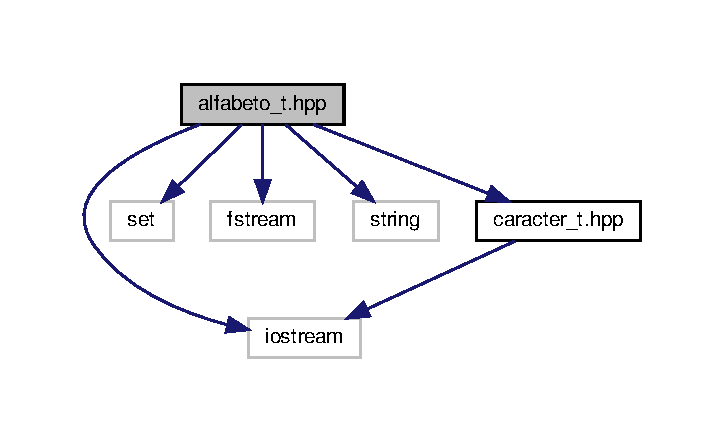
\includegraphics[width=348pt]{alfabeto__t_8hpp__incl}
\end{center}
\end{figure}
This graph shows which files directly or indirectly include this file\+:
\nopagebreak
\begin{figure}[H]
\begin{center}
\leavevmode
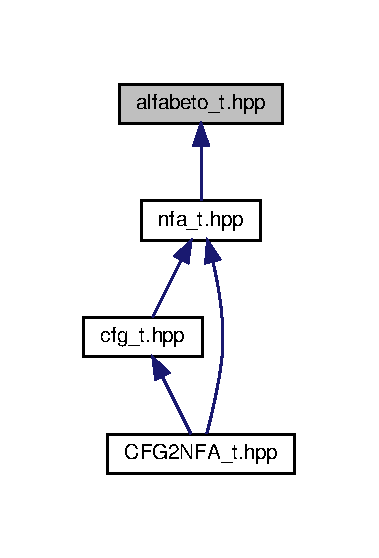
\includegraphics[width=182pt]{alfabeto__t_8hpp__dep__incl}
\end{center}
\end{figure}
\subsection*{Classes}
\begin{DoxyCompactItemize}
\item 
class \hyperlink{classalfabeto__t}{alfabeto\+\_\+t}
\end{DoxyCompactItemize}


\subsection{Detailed Description}
\begin{DoxyVersion}{Version}
1.\+0 
\end{DoxyVersion}
\begin{DoxyDate}{Date}
10/11/2019 
\end{DoxyDate}
\begin{DoxyAuthor}{Author}
Angel Julián Bolaño Campos  Gramáticas Regulares y Autómatas Finitos 
\end{DoxyAuthor}

\hypertarget{cadena__t_8hpp}{}\section{cadena\+\_\+t.\+hpp File Reference}
\label{cadena__t_8hpp}\index{cadena\+\_\+t.\+hpp@{cadena\+\_\+t.\+hpp}}
{\ttfamily \#include $<$iostream$>$}\newline
{\ttfamily \#include \char`\"{}symbol\+\_\+t.\+hpp\char`\"{}}\newline
{\ttfamily \#include $<$vector$>$}\newline
Include dependency graph for cadena\+\_\+t.\+hpp\+:
\nopagebreak
\begin{figure}[H]
\begin{center}
\leavevmode
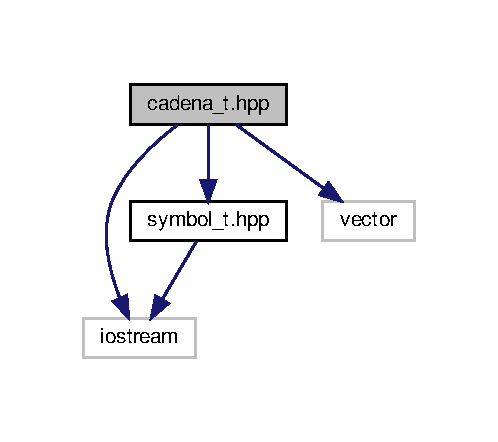
\includegraphics[width=239pt]{cadena__t_8hpp__incl}
\end{center}
\end{figure}
This graph shows which files directly or indirectly include this file\+:
\nopagebreak
\begin{figure}[H]
\begin{center}
\leavevmode
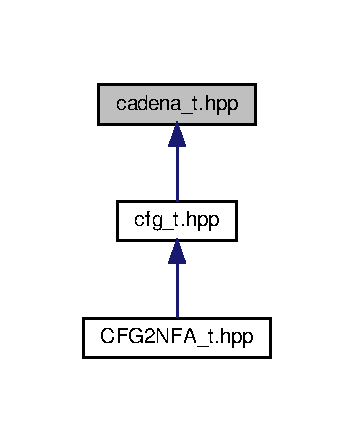
\includegraphics[width=170pt]{cadena__t_8hpp__dep__incl}
\end{center}
\end{figure}
\subsection*{Classes}
\begin{DoxyCompactItemize}
\item 
class \hyperlink{classcadena__t}{cadena\+\_\+t}
\end{DoxyCompactItemize}


\subsection{Detailed Description}
\begin{DoxyVersion}{Version}
1.\+0 
\end{DoxyVersion}
\begin{DoxyDate}{Date}
10/11/2019 
\end{DoxyDate}
\begin{DoxyAuthor}{Author}
Angel Julián Bolaño Campos  Gramáticas Regulares y Autómatas Finitos 
\end{DoxyAuthor}

\hypertarget{caracter__t_8hpp}{}\section{caracter\+\_\+t.\+hpp File Reference}
\label{caracter__t_8hpp}\index{caracter\+\_\+t.\+hpp@{caracter\+\_\+t.\+hpp}}
{\ttfamily \#include $<$iostream$>$}\newline
Include dependency graph for caracter\+\_\+t.\+hpp\+:
\nopagebreak
\begin{figure}[H]
\begin{center}
\leavevmode
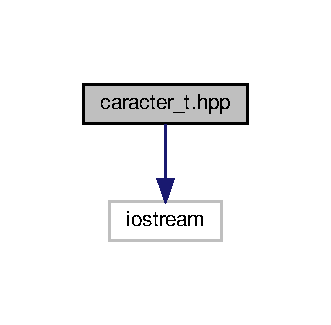
\includegraphics[width=159pt]{caracter__t_8hpp__incl}
\end{center}
\end{figure}
This graph shows which files directly or indirectly include this file\+:
\nopagebreak
\begin{figure}[H]
\begin{center}
\leavevmode
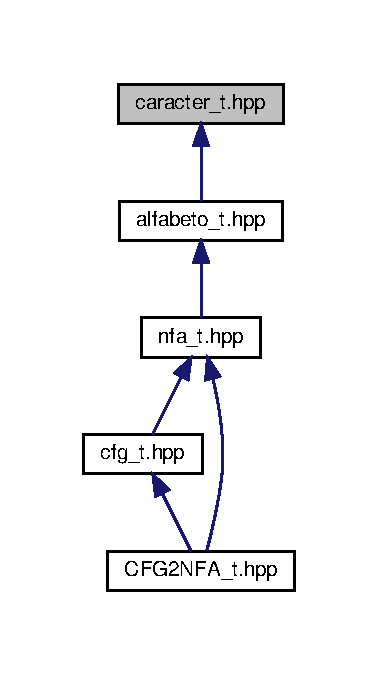
\includegraphics[width=182pt]{caracter__t_8hpp__dep__incl}
\end{center}
\end{figure}
\subsection*{Classes}
\begin{DoxyCompactItemize}
\item 
class \hyperlink{classcaracter__t}{caracter\+\_\+t}
\end{DoxyCompactItemize}
\subsection*{Enumerations}
\begin{DoxyCompactItemize}
\item 
\mbox{\Hypertarget{caracter__t_8hpp_a030a181134e163cb2a9e98e83810bb54}\label{caracter__t_8hpp_a030a181134e163cb2a9e98e83810bb54}} 
enum {\bfseries tipo} \{ {\bfseries O\+P\+E\+R\+A\+N\+DO}, 
{\bfseries O\+P\+E\+R\+A\+D\+OR}
 \}
\item 
\mbox{\Hypertarget{caracter__t_8hpp_ab4ae8eba5d6f887391b5539cae907990}\label{caracter__t_8hpp_ab4ae8eba5d6f887391b5539cae907990}} 
enum {\bfseries aridad} \{ {\bfseries U\+N\+A\+R\+IO} =1, 
{\bfseries B\+I\+N\+A\+R\+IO} =2
 \}
\end{DoxyCompactItemize}


\subsection{Detailed Description}
\begin{DoxyVersion}{Version}
1.\+0 
\end{DoxyVersion}
\begin{DoxyDate}{Date}
10/11/2019 
\end{DoxyDate}
\begin{DoxyAuthor}{Author}
Angel Julián Bolaño Campos  Gramáticas Regulares y Autómatas Finitos 
\end{DoxyAuthor}

\hypertarget{CFG2NFA__t_8hpp}{}\section{C\+F\+G2\+N\+F\+A\+\_\+t.\+hpp File Reference}
\label{CFG2NFA__t_8hpp}\index{C\+F\+G2\+N\+F\+A\+\_\+t.\+hpp@{C\+F\+G2\+N\+F\+A\+\_\+t.\+hpp}}
{\ttfamily \#include $<$iostream$>$}\newline
{\ttfamily \#include $<$fstream$>$}\newline
{\ttfamily \#include $<$string$>$}\newline
{\ttfamily \#include \char`\"{}cfg\+\_\+t.\+hpp\char`\"{}}\newline
{\ttfamily \#include \char`\"{}nfa\+\_\+t.\+hpp\char`\"{}}\newline
Include dependency graph for C\+F\+G2\+N\+F\+A\+\_\+t.\+hpp\+:
\nopagebreak
\begin{figure}[H]
\begin{center}
\leavevmode
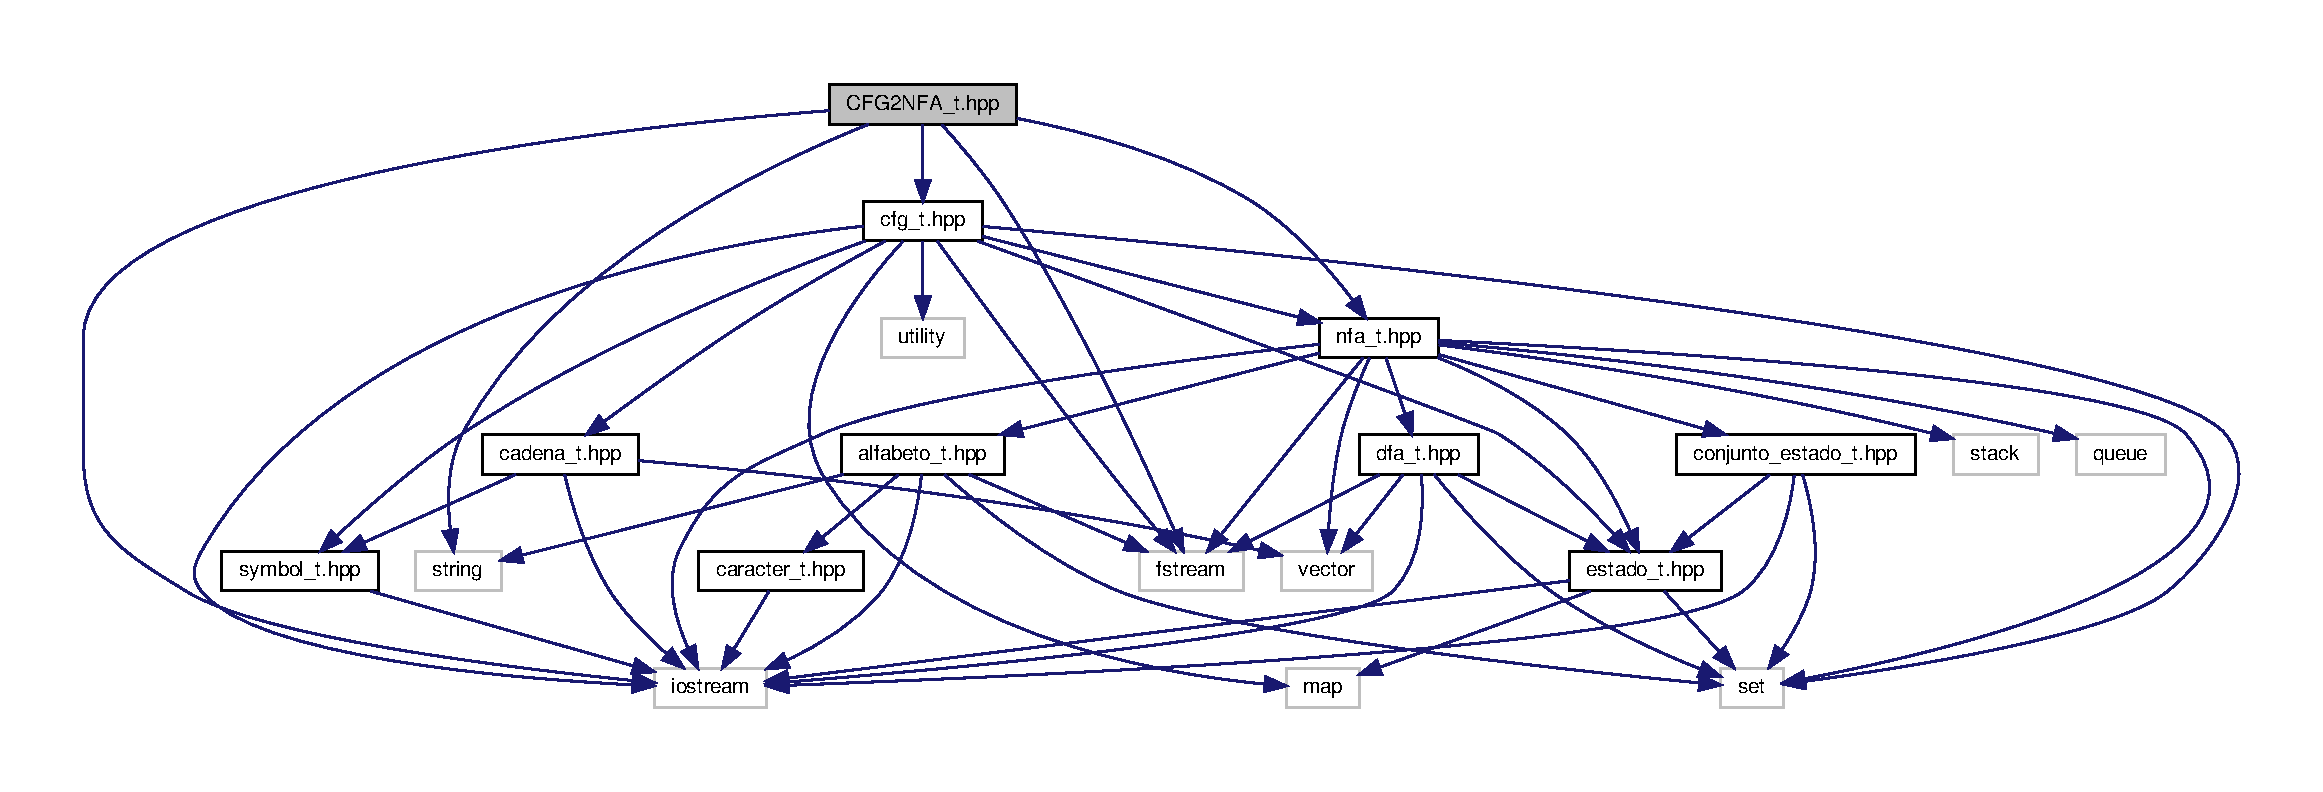
\includegraphics[width=350pt]{CFG2NFA__t_8hpp__incl}
\end{center}
\end{figure}
\subsection*{Classes}
\begin{DoxyCompactItemize}
\item 
class \hyperlink{classCFG2NFA__t}{C\+F\+G2\+N\+F\+A\+\_\+t}
\end{DoxyCompactItemize}


\subsection{Detailed Description}
\begin{DoxyVersion}{Version}
1.\+0 
\end{DoxyVersion}
\begin{DoxyDate}{Date}
10/11/2019 
\end{DoxyDate}
\begin{DoxyAuthor}{Author}
Angel Julián Bolaño Campos  Gramáticas Regulares y Autómatas Finitos 
\end{DoxyAuthor}

\hypertarget{cfg__t_8hpp}{}\section{cfg\+\_\+t.\+hpp File Reference}
\label{cfg__t_8hpp}\index{cfg\+\_\+t.\+hpp@{cfg\+\_\+t.\+hpp}}
{\ttfamily \#include $<$set$>$}\newline
{\ttfamily \#include $<$map$>$}\newline
{\ttfamily \#include $<$iostream$>$}\newline
{\ttfamily \#include $<$fstream$>$}\newline
{\ttfamily \#include $<$utility$>$}\newline
{\ttfamily \#include \char`\"{}cadena\+\_\+t.\+hpp\char`\"{}}\newline
{\ttfamily \#include \char`\"{}symbol\+\_\+t.\+hpp\char`\"{}}\newline
{\ttfamily \#include \char`\"{}nfa\+\_\+t.\+hpp\char`\"{}}\newline
{\ttfamily \#include \char`\"{}estado\+\_\+t.\+hpp\char`\"{}}\newline
Include dependency graph for cfg\+\_\+t.\+hpp\+:
\nopagebreak
\begin{figure}[H]
\begin{center}
\leavevmode
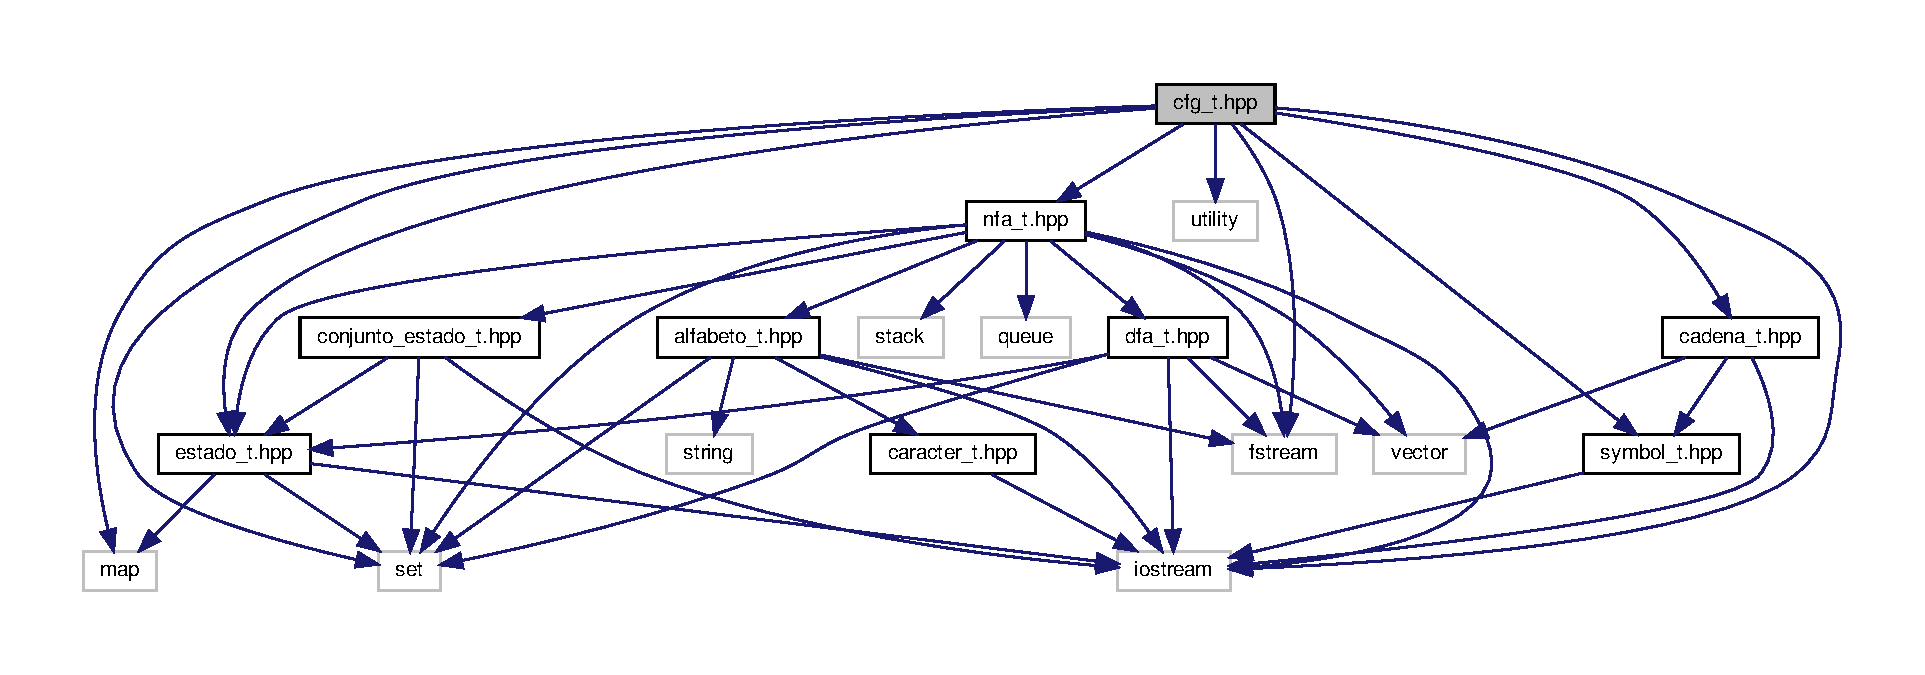
\includegraphics[width=350pt]{cfg__t_8hpp__incl}
\end{center}
\end{figure}
This graph shows which files directly or indirectly include this file\+:
\nopagebreak
\begin{figure}[H]
\begin{center}
\leavevmode
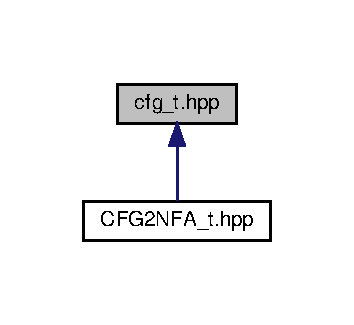
\includegraphics[width=170pt]{cfg__t_8hpp__dep__incl}
\end{center}
\end{figure}
\subsection*{Classes}
\begin{DoxyCompactItemize}
\item 
struct \hyperlink{structchecker}{checker}
\item 
class \hyperlink{classcfg__t}{cfg\+\_\+t}
\end{DoxyCompactItemize}
\subsection*{Typedefs}
\begin{DoxyCompactItemize}
\item 
\mbox{\Hypertarget{cfg__t_8hpp_ab898a226b4859c6b05508978c31366a3}\label{cfg__t_8hpp_ab898a226b4859c6b05508978c31366a3}} 
typedef std\+::map$<$ \hyperlink{classsymbol__t}{symbol\+\_\+t}, std\+::set$<$ \hyperlink{classcadena__t}{cadena\+\_\+t} $>$ $>$ {\bfseries produccion\+\_\+t}
\end{DoxyCompactItemize}


\subsection{Detailed Description}
\begin{DoxyVersion}{Version}
1.\+0 
\end{DoxyVersion}
\begin{DoxyDate}{Date}
10/11/2019 
\end{DoxyDate}
\begin{DoxyAuthor}{Author}
Angel Julián Bolaño Campos  Gramáticas Regulares y Autómatas Finitos 
\end{DoxyAuthor}

\hypertarget{conjunto__estado__t_8hpp}{}\section{conjunto\+\_\+estado\+\_\+t.\+hpp File Reference}
\label{conjunto__estado__t_8hpp}\index{conjunto\+\_\+estado\+\_\+t.\+hpp@{conjunto\+\_\+estado\+\_\+t.\+hpp}}
{\ttfamily \#include $<$set$>$}\newline
{\ttfamily \#include \char`\"{}estado\+\_\+t.\+hpp\char`\"{}}\newline
{\ttfamily \#include $<$iostream$>$}\newline
Include dependency graph for conjunto\+\_\+estado\+\_\+t.\+hpp\+:
\nopagebreak
\begin{figure}[H]
\begin{center}
\leavevmode
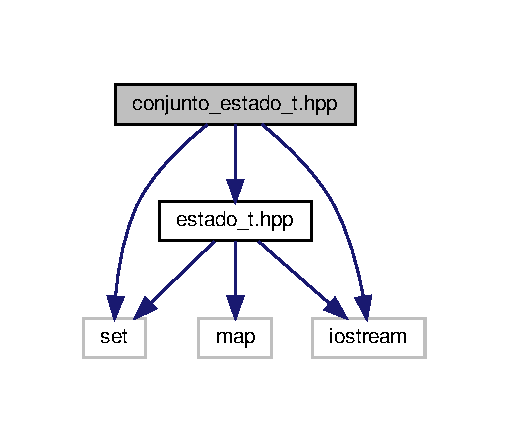
\includegraphics[width=244pt]{conjunto__estado__t_8hpp__incl}
\end{center}
\end{figure}
This graph shows which files directly or indirectly include this file\+:
\nopagebreak
\begin{figure}[H]
\begin{center}
\leavevmode
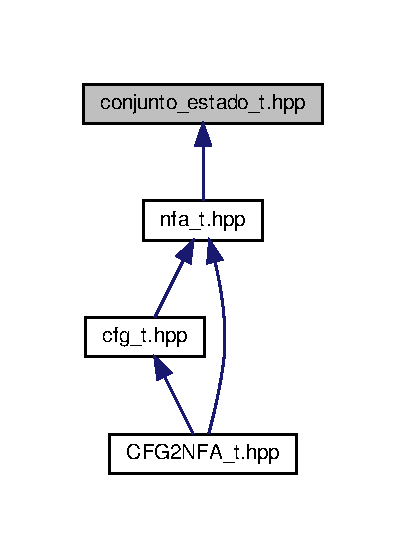
\includegraphics[width=195pt]{conjunto__estado__t_8hpp__dep__incl}
\end{center}
\end{figure}
\subsection*{Classes}
\begin{DoxyCompactItemize}
\item 
class \hyperlink{classcon__est__t}{con\+\_\+est\+\_\+t}
\end{DoxyCompactItemize}


\subsection{Detailed Description}
\begin{DoxyVersion}{Version}
1.\+0 
\end{DoxyVersion}
\begin{DoxyDate}{Date}
10/11/2019 
\end{DoxyDate}
\begin{DoxyAuthor}{Author}
Angel Julián Bolaño Campos  Gramáticas Regulares y Autómatas Finitos 
\end{DoxyAuthor}

\hypertarget{dfa__t_8hpp}{}\section{dfa\+\_\+t.\+hpp File Reference}
\label{dfa__t_8hpp}\index{dfa\+\_\+t.\+hpp@{dfa\+\_\+t.\+hpp}}
{\ttfamily \#include $<$set$>$}\newline
{\ttfamily \#include $<$iostream$>$}\newline
{\ttfamily \#include $<$fstream$>$}\newline
{\ttfamily \#include $<$vector$>$}\newline
{\ttfamily \#include \char`\"{}estado\+\_\+t.\+hpp\char`\"{}}\newline
Include dependency graph for dfa\+\_\+t.\+hpp\+:
\nopagebreak
\begin{figure}[H]
\begin{center}
\leavevmode
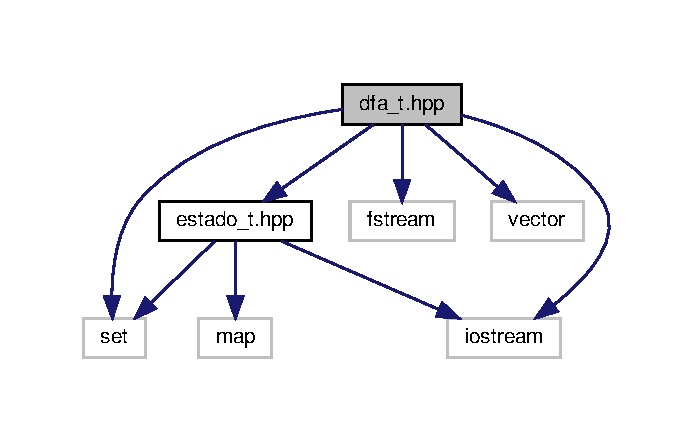
\includegraphics[width=333pt]{dfa__t_8hpp__incl}
\end{center}
\end{figure}
This graph shows which files directly or indirectly include this file\+:
\nopagebreak
\begin{figure}[H]
\begin{center}
\leavevmode
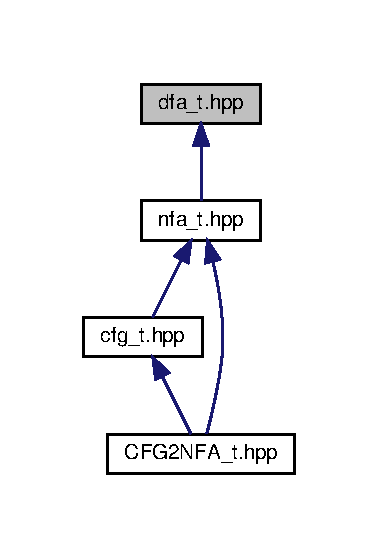
\includegraphics[width=182pt]{dfa__t_8hpp__dep__incl}
\end{center}
\end{figure}
\subsection*{Classes}
\begin{DoxyCompactItemize}
\item 
class \hyperlink{classdfa__t}{dfa\+\_\+t}
\end{DoxyCompactItemize}


\subsection{Detailed Description}
\begin{DoxyVersion}{Version}
1.\+0 
\end{DoxyVersion}
\begin{DoxyDate}{Date}
10/11/2019 
\end{DoxyDate}
\begin{DoxyAuthor}{Author}
Angel Julián Bolaño Campos  Gramáticas Regulares y Autómatas Finitos 
\end{DoxyAuthor}

\hypertarget{estado__t_8hpp}{}\section{estado\+\_\+t.\+hpp File Reference}
\label{estado__t_8hpp}\index{estado\+\_\+t.\+hpp@{estado\+\_\+t.\+hpp}}
{\ttfamily \#include $<$iostream$>$}\newline
{\ttfamily \#include $<$map$>$}\newline
{\ttfamily \#include $<$set$>$}\newline
Include dependency graph for estado\+\_\+t.\+hpp\+:
\nopagebreak
\begin{figure}[H]
\begin{center}
\leavevmode
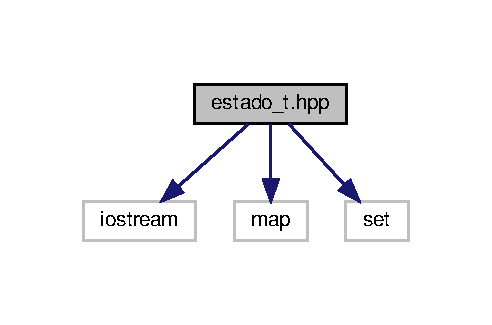
\includegraphics[width=236pt]{estado__t_8hpp__incl}
\end{center}
\end{figure}
This graph shows which files directly or indirectly include this file\+:
\nopagebreak
\begin{figure}[H]
\begin{center}
\leavevmode
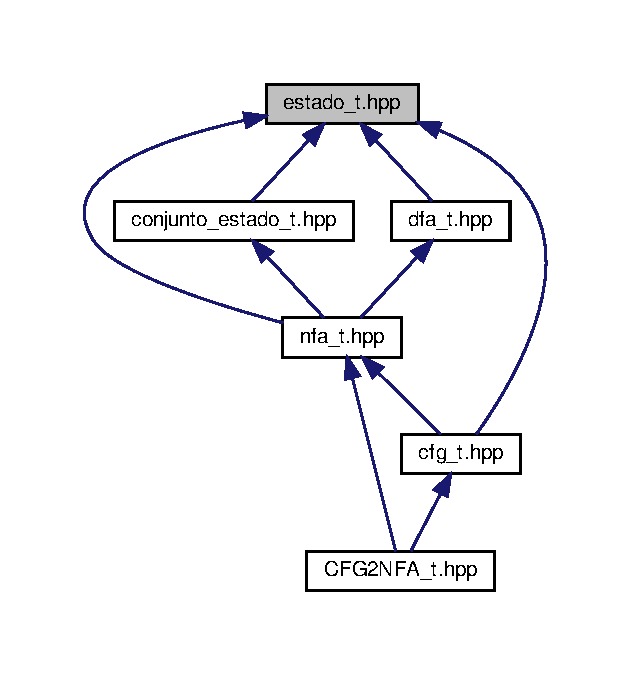
\includegraphics[width=302pt]{estado__t_8hpp__dep__incl}
\end{center}
\end{figure}
\subsection*{Classes}
\begin{DoxyCompactItemize}
\item 
class \hyperlink{classestado__t}{estado\+\_\+t}
\end{DoxyCompactItemize}
\subsection*{Typedefs}
\begin{DoxyCompactItemize}
\item 
\mbox{\Hypertarget{estado__t_8hpp_a50890574188e8493dfe5aa6f7c0ed842}\label{estado__t_8hpp_a50890574188e8493dfe5aa6f7c0ed842}} 
typedef std\+::map$<$ char, std\+::set$<$ \hyperlink{classestado__t}{estado\+\_\+t} $>$ $>$ {\bfseries trans\+\_\+map}
\end{DoxyCompactItemize}


\subsection{Detailed Description}
\begin{DoxyVersion}{Version}
1.\+0 
\end{DoxyVersion}
\begin{DoxyDate}{Date}
10/11/2019 
\end{DoxyDate}
\begin{DoxyAuthor}{Author}
Angel Julián Bolaño Campos  Gramáticas Regulares y Autómatas Finitos 
\end{DoxyAuthor}

\hypertarget{nfa__t_8hpp}{}\section{nfa\+\_\+t.\+hpp File Reference}
\label{nfa__t_8hpp}\index{nfa\+\_\+t.\+hpp@{nfa\+\_\+t.\+hpp}}
{\ttfamily \#include $<$iostream$>$}\newline
{\ttfamily \#include $<$fstream$>$}\newline
{\ttfamily \#include $<$set$>$}\newline
{\ttfamily \#include $<$vector$>$}\newline
{\ttfamily \#include $<$stack$>$}\newline
{\ttfamily \#include $<$queue$>$}\newline
{\ttfamily \#include \char`\"{}estado\+\_\+t.\+hpp\char`\"{}}\newline
{\ttfamily \#include \char`\"{}conjunto\+\_\+estado\+\_\+t.\+hpp\char`\"{}}\newline
{\ttfamily \#include \char`\"{}dfa\+\_\+t.\+hpp\char`\"{}}\newline
{\ttfamily \#include \char`\"{}alfabeto\+\_\+t.\+hpp\char`\"{}}\newline
Include dependency graph for nfa\+\_\+t.\+hpp\+:
\nopagebreak
\begin{figure}[H]
\begin{center}
\leavevmode
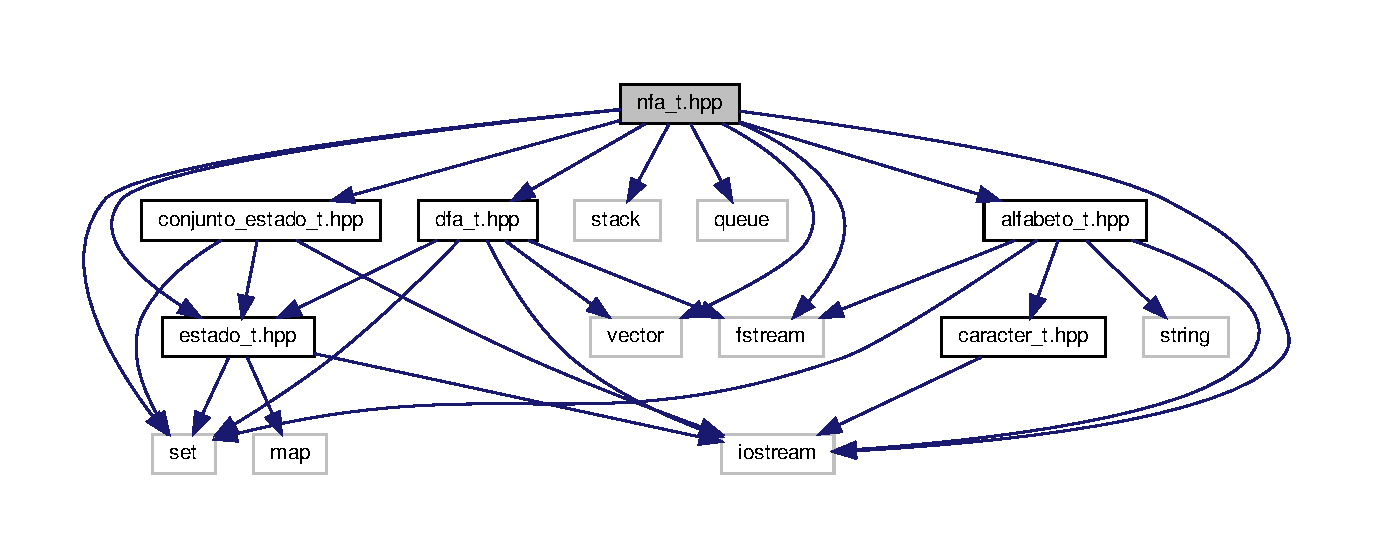
\includegraphics[width=350pt]{nfa__t_8hpp__incl}
\end{center}
\end{figure}
This graph shows which files directly or indirectly include this file\+:
\nopagebreak
\begin{figure}[H]
\begin{center}
\leavevmode
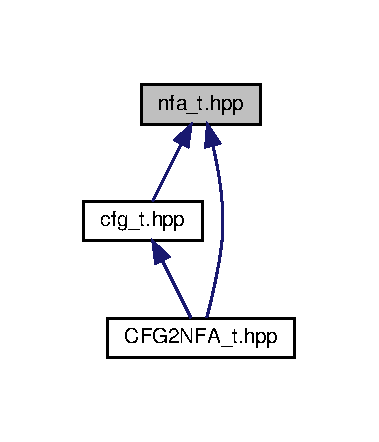
\includegraphics[width=182pt]{nfa__t_8hpp__dep__incl}
\end{center}
\end{figure}
\subsection*{Classes}
\begin{DoxyCompactItemize}
\item 
class \hyperlink{classnfa__t}{nfa\+\_\+t}
\end{DoxyCompactItemize}
\subsection*{Variables}
\begin{DoxyCompactItemize}
\item 
\mbox{\Hypertarget{nfa__t_8hpp_ae2e30439684674a6b9acc58937ad8eca}\label{nfa__t_8hpp_ae2e30439684674a6b9acc58937ad8eca}} 
const char {\bfseries E\+PS} = \textquotesingle{}$\sim$\textquotesingle{}
\end{DoxyCompactItemize}


\subsection{Detailed Description}
\begin{DoxyVersion}{Version}
1.\+0 
\end{DoxyVersion}
\begin{DoxyDate}{Date}
10/11/2019 
\end{DoxyDate}
\begin{DoxyAuthor}{Author}
Angel Julián Bolaño Campos  Gramáticas Regulares y Autómatas Finitos 
\end{DoxyAuthor}

\hypertarget{symbol__t_8hpp}{}\section{symbol\+\_\+t.\+hpp File Reference}
\label{symbol__t_8hpp}\index{symbol\+\_\+t.\+hpp@{symbol\+\_\+t.\+hpp}}
{\ttfamily \#include $<$iostream$>$}\newline
Include dependency graph for symbol\+\_\+t.\+hpp\+:
\nopagebreak
\begin{figure}[H]
\begin{center}
\leavevmode
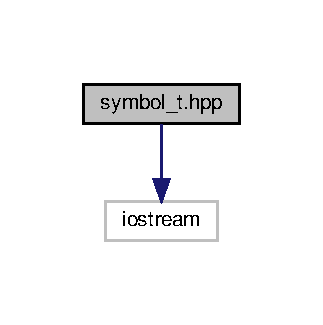
\includegraphics[width=155pt]{symbol__t_8hpp__incl}
\end{center}
\end{figure}
This graph shows which files directly or indirectly include this file\+:
\nopagebreak
\begin{figure}[H]
\begin{center}
\leavevmode
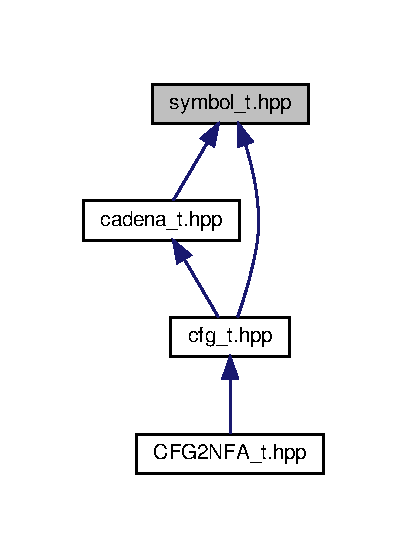
\includegraphics[width=196pt]{symbol__t_8hpp__dep__incl}
\end{center}
\end{figure}
\subsection*{Classes}
\begin{DoxyCompactItemize}
\item 
class \hyperlink{classsymbol__t}{symbol\+\_\+t}
\end{DoxyCompactItemize}


\subsection{Detailed Description}
\begin{DoxyVersion}{Version}
1.\+0 
\end{DoxyVersion}
\begin{DoxyDate}{Date}
10/11/2019 
\end{DoxyDate}
\begin{DoxyAuthor}{Author}
Angel Julián Bolaño Campos  Gramáticas Regulares y Autómatas Finitos 
\end{DoxyAuthor}

%--- End generated contents ---

% Index
\backmatter
\newpage
\phantomsection
\clearemptydoublepage
\addcontentsline{toc}{chapter}{Index}
\printindex

\end{document}
